% Author: Brandon Patterson
% Description: Dissertation
%
%
% Use the University of Michigan thesis class.
\documentclass[submit]{./tex/thesis-umich}


% Title of the thesis
\title{Applications of Computation in Acoustics: Ultrasound Bioeffects and Underwater Transmission Loss Uncertainty}
%\title{Computational investigations of ultrasound bioeffects and related physics}
%\title{Acoustically-driven fluid interfaces with applications to diagnostic ultrasound bioeffects}



% Author name
\author{Brandon Patterson}

% Department
\department{(Mechanical Engineering)}

% Year of completion
\year=\the\year

% Frontispiece
\frontispiece{\includegraphics[width=4in]{./figs/frontispiece/brooke_nobackground}}

% Default style for front pages
\frontpagestyle{1}

%% Dedication
\dedication{\topskip0pt
\pagebreak
\vspace*{\fill}
\begin{center}
  To Dad
\end{center}
\vspace*{\fill}
\pagebreak

%%% Local Variables:
%%% mode: latex
%%% TeX-master: "../main"
%%% End:
}

%% Acknowledgments
\acknowledgments{\include{./content/Acknowledgements}}%

% This command sets the width of the acknowledgments area as a fraction
% of the total width of the text area.
\acknowledgmentswidth{0.75}%

% Preface
%\preface[2]{\include{./content/preface}}%
\preface{\include{./content/preface}}%

% Committee
\committee{%
\hspace*{12pt} Professor David R. Dowling, Co-Chair\\%, Mechanical Engineering, University of Michigan\\
\hspace*{12pt} Associate Professor Eric Johnsen, Co-Chair\\
\hspace*{12pt} Professor J. Brian Fowlkes\\
\hspace*{12pt} Professor Douglas L. Miller\\%, Radiology, University of Michigan
\hspace*{12pt} Professor William Schultz\\%, Mechanical Engineering, University of Michigan\\
}

%% Chair must be entered separately for formatting reasons.
\chair{Eric Johnsen}
\cochair{David R. Dowling \& Eric Johnsen}

%% What deliverable requirement does this fill
\deliverable{Dissertation}

% Commands to hide or show lists of figures, tables, etc.
% \hidelistoftables
% \hidelistofprograms
% \hidelistofappendices
% \hidelistoffigures
% \hidelistofabbreviations
% \hidelistofacronyms
% \hidededication

\showlistoftables
%\showlistofprograms
%\showlistofappendices
\showlistofabbreviations
\showlistoffigures
\showacknowledgments


%% Definition of any abbreviations used.
\abbreviations{
 \acro{CEUS}{Contrast-Enhanced Ultrasound}
 \acro{CFD}{Computational Fluid Dynamics}
 \acro{DG}{Discontinuous Galerkin}
 \acro{DUS}{Diagnostic Ultrasound}
 \acro{ED}{Exposure Duration}
 \acro{FDA}{Food and Drug Administration}
 \acro{HIFU}{High-Intensity Focused Ultrasound}
 \acro{IC}{Inertial Cavitation} 
 \acro{LH}{Lung hemorrhage}
 \acro{MC}{Monte Carlo}
 \acro{MI}{Mechanical Index}
 \acro{PCH}{Pulmonary Capillary Hemorrhage}
 \acro{PH}{Pulmonary Hemorrhage}
 \acro{PD}{Pulse Duration}
 \acro{PDF}{Probability Density Function}
 \acro{PFP}{Perfluoropropane}
 \acro{PRF}{Pulse Repetition Frequency}
 \acro{PRPA}{Peak Rarefaction Pressure Amplitude}
 \acro{RM}{Richtmyer-Meshkov}
 \acro{RMI}{Richtmyer-Meshkov Instability}
 \acro{RT}{Rayleigh-Taylor}
 \acro{RTI}{Rayleigh-Taylor Instability}
 \acro{STEM}{Science, Technology, Engineering, and Math}
 \acro{TL}{Transmission Loss}
 \acro{US}{Ultrasound}
 \acro{WENO}{Weighted Essentially non-oscillatory}


%%% Local Variables:
%%% mode: latex
%%% TeX-master: "../prelim"
%%% End:

}

%% Some abstract text
%\abstract{\begin{center}
  \begin{minipage}{0.8\textwidth}
    \subsection*{Abstract}
    \ac{DUS} has been shown to cause \ac{LH} in a variety of mammals,
    though the underlying damage mechanisms are still
    unclear. Motivated by this problem aim to investigate the physics
    underlying interactions between acoustic waves and liquid-gas
    interfaces such as those in the lung. We model an alveolar
    tissue-air interface as a perturbed water-air interface and
    simulate its interaction with trapezoidal acoustic waves to
    investigate the underlying physics. Though order of magnitude
    analysis and simulation, we show that baroclinic vorticity is
    generated within gas-dominated fluid at the interface, as a result
    of misalignment between acoustic pressure gradients and the
    interface density gradients. This vorticity deforms the interface
    long after all of the acoustic waves have passed. This nonlinear
    effect is has potential importance at liquid-gas interfaces
    because of the sharp density discontinuity. Dimensional analysis
    is performed to show that the amplitude of a purely
    circulation-driven interface will grow as $t^{0.5}$. This result
    is compared to computational results obtained for the acoustically
    driven interface perturbation which appears to grow as
    $t^{0.6}$ at late time. \par
    
    \hspace*{4ex} Additionally we subject water-air interfaces to
    waves of similar size and amplitude, but varying duration to
    demonstrate that interface deformation that occurs during the
    wave-interface interaction appreciably changes the long-term
    dynamics of the interface by altering the vorticity
    deposition. This effect is relevant to acoustic waves in
    particular, which travel occupy a finite amount of space, and
    hence interact with the interface over variable, finite amounts of
    time. This is in contrast to the well studied shock-interface
    interactions, which occur nearly instantaneously.
  \end{minipage}
\end{center}
%%% Local Variables:
%%% mode: latex
%%% TeX-master: "../main"
%%% End:
}
\abstract{\input{./content/abstract550}}
\showabstractpagenumber

%\usepackage{fullpage}
\usepackage{hyperref}
\usepackage{graphicx}
\usepackage{natbib}
\usepackage{pdflscape}
\usepackage{mathrsfs}
\usepackage{rotating}
\usepackage[usenames,dvipsnames]{xcolor}
\usepackage{tikz}
\usepackage{pgfgantt}
%\usepackage{typearea}
\usepackage{booktabs}
\usepackage{abstract} \usepackage{verbatim} \usepackage{tabularx}
\usepackage{caption} \usepackage{subcaption} \usepackage{embedfile}
\usepackage{import} \usepackage[normalem]{ulem}
\usepackage[toc,page]{appendix}
%\usepackage]{appendix}
\usepackage{titlesec}
\usepackage{adjustbox} \usepackage{hhline} \usepackage{ragged2e} \usepackage{setspace} \usepackage{multirow}%Needed to make tables converted from word working 
\usepackage{totcount}
\usepackage{transparent}
\usepackage{txfonts}


% My commands
\newcommand{\ganttgroupc}[5][none]{\ganttgroup[group/.append style={draw=black, fill=#1}, group incomplete/.append style={draw=black,fill=#1!50}, progress=#2]{#3}{#4}{#5}}
\newcommand{\ganttbarc}[5][none]{\ganttbar[bar/.append style={draw=black, fill=#1}, bar incomplete/.append style={draw=black,fill=#1!50}, progress=#2]{#3}{#4}{#5}}
\newcommand{\bs}[1]{\boldsymbol{#1}}
\newcommand{\mcbs}[1]{\boldsymbol{\mathcal{#1}}}
\newcommand{\mbbs}[1]{\boldsymbol{\mathbf{#1}}}
\newcommand{\del}[0]{\nabla}
\newcommand{\orderof}[1]{\ensuremath{\mathcal{O}\left(#1\right)}}
\newcommand{\abs}[1]{\ensuremath{\left|#1\right|}}
\newcommand{\norm}[1]{\ensuremath{\left\Vert#1\right\Vert}}
\newcommand{\plus}{\raisebox{.2\height}{\scalebox{.8}{+}}}
\newcommand*\diff{\mathop{}\!\mathrm{d}}
\newcommand*\Diff[1]{\mathop{}\!\mathrm{d^#1}}

% Used to count references
\newtotcounter{citnum} %From the totcount package documentation
\def\oldbibitem{} \let\oldbibitem=\bibitem
\def\bibitem{\stepcounter{citnum}\oldbibitem}

% Used to get section names
\let\Sectionmark\sectionmark
\def\sectionmark#1{\def\Sectionname{#1}\Sectionmark{#1}}
\let\Subsectionmark\subsectionmark
\def\subsectionmark#1{\def\Subsectionname{#1}\Subsectionmark{#1}}

%% Declare math operators
\DeclareMathOperator{\sech}{sech}
\DeclareMathOperator{\csch}{csch}
\DeclareMathOperator{\arcsec}{arcsec}
\DeclareMathOperator{\arccot}{arcCot}
\DeclareMathOperator{\arccsc}{arcCsc}
\DeclareMathOperator{\arccosh}{arcCosh}
\DeclareMathOperator{\arcsinh}{arcsinh}
\DeclareMathOperator{\arctanh}{arctanh}
\DeclareMathOperator{\arcsech}{arcsech}
\DeclareMathOperator{\arccsch}{arcCsch}
\DeclareMathOperator{\arccoth}{arcCoth}  

% New table columns
\newcolumntype{L}[1]{>{\raggedright\let\newline\\\arraybackslash\hspace{0pt}}m{#1}}
\newcolumntype{C}[1]{>{\centering\let\newline\\\arraybackslash\hspace{0pt}}m{#1}}
\newcolumntype{R}[1]{>{\raggedleft\let\newline\\\arraybackslash\hspace{0pt}}m{#1}}

% Preferentially use .pdf files when other formats are available (default preference w/o this line is .png, then pdf, etc...
\DeclareGraphicsExtensions{.pdf,.PDF,.png,.PNG,.jpg,.mps,.jpeg,.jbig2,.jb2,.JPG,.JPEG,.JBIG2,.JB2}



% Create a snapshot of dependencies and place in .dep file
\RequirePackage{snapshot}

% Embed files
%%\embedfile{./Content/Dedication}
\embedfile{./embed_files.tex}
%\embedfile{./content/acknowledgements.tex}
\embedfile{./content/abstract.tex}
%\embedfile{./content/foreword.tex}
\embedfile{./content/abstract.tex}
\embedfile{./content/acronyms.tex}
\embedfile{./content/chapters/intro_chapter.tex}
\embedfile{./content/chapters/usbe_bubble_abstract.tex}
\embedfile{./content/chapters/usbe_bubble_key.tex}
\embedfile{./content/chapters/usbe_bubble_chapter.tex}
\embedfile{./content/chapters/usbe_lung_abstract.tex}
\embedfile{./content/chapters/usbe_lung_intro.tex}
\embedfile{./content/chapters/usbe_lung_methods.tex}
\embedfile{./content/chapters/usbe_lung_analysis.tex}
\embedfile{./content/chapters/usbe_lung_results.tex}
\embedfile{./content/chapters/usbe_lung_conclusions.tex}
\embedfile{./content/chapters/usbe_lung_future.tex}
\embedfile{./content/chapters/asuq_astats_key.tex}
\embedfile{./content/chapters/asuq_astats_abstract.tex}
\embedfile{./content/chapters/asuq_astats_intro.tex}
\embedfile{./content/chapters/asuq_astats_methods.tex}
\embedfile{./content/chapters/asuq_astats_results.tex}
\embedfile{./content/chapters/asuq_astats_conclusions.tex}
%                                                               
%
%%% Local Variables:
%%% mode: latex
%%% TeX-master: "prelim"
%%% End:

\embedfile{main.tex}

% Setup latexdiff
\input{./tex/diff_preamble.tex}

\setcounter{tocdepth}{5}
\setcounter{secnumdepth}{5}

\titleformat{\paragraph}
{\normalfont\normalsize\bfseries}{\theparagraph}{1em}{}
\titlespacing*{\paragraph}
{0pt}{3.25ex plus 1ex minus .2ex}{1.5ex plus .2ex}

% Fix subcaptions to look like (a)
\captionsetup{subrefformat=parens}

% Black citations for cheap printing
\hypersetup{citecolor=black}

%% DOCUMENT AREA

\begin{document}
%\chapter*{Foreword} \label{ch:foreword}
%\input{./content/foreword.tex}


%Abstract
%\begin{center}
  \begin{minipage}{0.8\textwidth}
    \subsection*{Abstract}
    \ac{DUS} has been shown to cause \ac{LH} in a variety of mammals,
    though the underlying damage mechanisms are still
    unclear. Motivated by this problem aim to investigate the physics
    underlying interactions between acoustic waves and liquid-gas
    interfaces such as those in the lung. We model an alveolar
    tissue-air interface as a perturbed water-air interface and
    simulate its interaction with trapezoidal acoustic waves to
    investigate the underlying physics. Though order of magnitude
    analysis and simulation, we show that baroclinic vorticity is
    generated within gas-dominated fluid at the interface, as a result
    of misalignment between acoustic pressure gradients and the
    interface density gradients. This vorticity deforms the interface
    long after all of the acoustic waves have passed. This nonlinear
    effect is has potential importance at liquid-gas interfaces
    because of the sharp density discontinuity. Dimensional analysis
    is performed to show that the amplitude of a purely
    circulation-driven interface will grow as $t^{0.5}$. This result
    is compared to computational results obtained for the acoustically
    driven interface perturbation which appears to grow as
    $t^{0.6}$ at late time. \par
    
    \hspace*{4ex} Additionally we subject water-air interfaces to
    waves of similar size and amplitude, but varying duration to
    demonstrate that interface deformation that occurs during the
    wave-interface interaction appreciably changes the long-term
    dynamics of the interface by altering the vorticity
    deposition. This effect is relevant to acoustic waves in
    particular, which travel occupy a finite amount of space, and
    hence interact with the interface over variable, finite amounts of
    time. This is in contrast to the well studied shock-interface
    interactions, which occur nearly instantaneously.
  \end{minipage}
\end{center}
%%% Local Variables:
%%% mode: latex
%%% TeX-master: "../main"
%%% End:

\acresetall

\renewcommand\thepart{Part~\Roman{part}:} %%%%%%%%%%%%%%%%%%%%%%%%%%%%%%%%% WORKED FOR TOC, but broke things later
\renewcommand\cftpartpresnum{Part~}
% % US Bioeffects
\part{Ultrasound bioeffects} \label{part:ultrasound_bioeffects}
%\chapter{Introduction to ultrasound bioeffects} \label{ch:usbe_intro}%
The purpose of this chapter is twofold. First, I provide a brief
introduction to ultrasound and related biological effects to provide
physical context for this work. Second, I offer a brief overview of
the work to be presented and its significance. For a more detailed
overview of the relevant literature, the reader is referred to later
parts of this document, and to this authors published works.

\section{Physical context} \label{sec:usbe_intro_physical_context}%
Diagnostic \ac{US} has proven to be among the safest and most powerful
medical imaging tools currently available \hl{CITE}. Its use has become
ubiquitous throughout modern medicine. The basic physical principle
underlying this technology is the scattering of sound at material
interfaces. In practice, high-frequency, typically MHz range, acoustic
waves and pulses are created at the surface of the body using a
piezoelectric \ac{US} transducer. These vibrations propagate via an
acoustic coupling medium from the transducer into the tissue and
scatter at changes in the material properties of the medium. More
simply, some of the sound echoes whenever it moves from one tissue to
another, or hits a cavity in the body. These echoes are then picked up
by a receiver and recorded. This echo signal is processed to obtain
real-time images of the scattering surface.

While clinical \ac{US} is typically safe there are specific instances
during which \ac{US} can interact with tissue in such a way that the
tissue is physically altered. These effects to the body are referred
to as \ac{US} bioeffects. Understanding these \ac{US}-tissue
interactions is important for the development of safe, effective
\ac{US} techniques \citep{Dalecki2004}. While the entire field of
therapeutic \ac{US} is focused on intentionally causing bioeffects in
a way that is beneficial to the patient, diagnostic \ac{US} is a
different story. Bioeffects that occur during diagnostic \ac{US}
typically take the form of unintended hemorrhage, tissue damage, or
cell death. Depending on the physical damage mechanism responsible,
these bioeffects are broadly classified into two groups, thermal and
non-thermal \citep{OBrien2007}. The first group, thermal bioeffects
are characterized by deposition of acoustic energy into tissue as heat
via viscous dissipation. At the cellular and molecular scales, this
can lead to the release of highly reactive free radicals, protein
denaturation, and ultimately tissue damage and death. Little else will
be said about thermal bioeffects, as the bioeffects problems of
interest to this work are a result of non-thermal mechanisms.

The bulk of known non-thermal bioeffects are attributed to
acoustically-induced cavitation. Acoustic cavitation is the phenomenon
by which gas nano and microbubbles, called cavitation nuclei, are
cyclically grown by low pressures within the \ac{US} field and then
collapsed high pressures within the field. Cavitation can be divided
into two categories, stable cavitation, also called gas body
activation, and \ac{IC}, formerly referred to as transient
cavitation. Stable cavitation typically occurs for low \ac{US}
intensity an is characterized by bubbles periodically oscillating
around an equilibrium radius for multiple acoustic cycles. \ac{IC}
typically occurs for higher ultrasound intensities. During \ac{IC} the
bubble dynamics during collapse are dominated by the inertia of the
surrounding fluid. The bubble collapses violently to a tiny fraction
of its original size and then explosively rebounds back. There are
variety of physical phenomena associated with \ac{IC} that may be
responsible for observed \ac{US} bioeffects. Upon collapse, the
pressure and temperature within the bubbles spike, often reaching
billions of pascals and thousands of Kelvin respectively. Due to the
pressure difference between the vapor/gas mixture within the bubble at
collapse and the surrounding media, the collapsed bubble can emit a
powerful shock wave. When cavitation is triggered near a rigid
surface, the bubble can collapse in a radially asymmetric fashion
causing a high speed ``re-entrant'' jet of liquid to impinge upon the
surface, effectively striking the surface with a liquid hammer. If
cavitation occurs at an appropriate distance from a non-rigid surface,
such as soft tissue boundaries and blood vessel walls, the jet can
impinge away from the surface, potentially invaginating the surface
\citep{Brujan2011}. One type of \ac{DUS} for which cavitation is of
particular concern is \ac{CEUS}, which uses contrast-agent
microbubbles injected into patients bloodstream to act as additional
scattering surfaces. These microbubbles can also serve as cavitation
nuclei and have been associated with a variety of \ac{US} bioeffects. 

\hl{
 MECHANICAL INDEX PARAGRAPH:} As a result of the potential for
  cavitation-related \ac{US} bioeffects the United States Food and
  Drug Administration called for a metric to predict likely cavitation
  damage from ultrasound. As bioeffects are typically attributed to
  \ac{IC}, efforts to predict cavitation damage considered the
  likelihood of \ac{IC} based on theoretical calculations of free gas
  bubbles in water. In the case of acoustic cavitation, this depends
  on the duration of peak negative pressure experienced by a
  cavitation nucleus, with longer interactions depositing more energy
  into the nucleus, and thus having a greater likelihood inducing
  \ac{IC}. The duration of the \ac{PRPA} is inversely related to the
  \ac{US} frequency. \cite{Holland1989} demonstrated that the
  threshold \ac{PRPA} needed to trigger \ac{IC}, defined based on a
  maximum bubble temperature $\geq5000$K, depended on the size of the
  cavitation nucleus. Smaller cavitation nucleii, must overcome
  greater surface tension effects in order to cavitate, with the
  Laplace pressure scaling inversely with the radius of the
  nucleus. Furthermore, as initial radius a nucleus increases, the
  inertia of the surrounding fluid that must be overcome also
  increases\cite{AiumS72000}. Thus \cite{Holland1989} illustrated that
  for a given frequency their is an optimal nucleus size for
  triggering \ac{IC}. Based on these calculations and corrections for
  heat dissipation in tissue the \ac{MI} was created as a measure of
  ultrasound induced cavitation related bioeffects and defined as 
  \begin{align}
    MI = \frac{P_{r.3}}{\sqrt{f_c}},
  \end{align}
  where $P_{r.3}$ is the \ac{PRPA} derated by $0.3$ dB/MHz-cm and
  $f_c$ is the center frequency \cite{Apfel1991}. The United States
  \ac{FDA} mandates that $MI\leq1.9$ for diagnostic imaging, though
  \ac{US} bioeffects have been observed at \ac{MI} below this in case
  of \ac{DUS} of mammalian lungs.


Another non-thermal \ac{US} bioeffect of interest is \ac{DUS}-induced
\ac{LH}, which is the only known bioeffect of non-contrast \ac{DUS}
known to occur in mammals. Despite the fact that this phenomenon was
first observed in mice over twenty years ago \citep{Child1990}, the
underlying physical damage mechanisms remain unknown. Research has
shown that thermal damage mechanisms are unlikely as \ac{DUS}-induced
lung lesions do not appear similar to those induced by heat
\citep{Zachary2006}. Furthermore, cavitation mechanisms do not appear
to be responsible, as the severity of \ac{DUS}-induced \ac{LH} in mice
increased under raised hydrostatic pressure \citep{OBrien2000} and was
unaffected by the introduction of \ac{US} contrast agents into
subjects. Both of these results are inconsistent with what is expected
of \ac{IC}-induced bioeffects. Works by \cite{Tjan2007,Tjan2008} model
the evolution of an inviscid, free surface subjected to a Gaussian
velocity potential and find that this can lead to the ejection of
liquid droplets. They go on to say that \ac{DUS} of the lung may
similarly lead to the ejected of droplets capable of puncturing the
air-filled sacs within the lung. This problem is central to the our
present and future work, and makes up the bulk of this proposal. As
such, a far more in-depth literature review will be provided in
Chapter \ref{ch:usbe_lung}.

\section{An overview the present work}
\label{sec:usbe_intro_overview}%
This dissertation focuses on two specific problems within the realm of
\ac{DUS}-related bioeffects and the underlying physics of
each. Specifically, we will consider contrast enhanced ultrasound and
\ac{DUS}-induced lung tissue.

First, in Chapter \ref{ch:usbe_bubble} we look at the problem of
contrast enhanced ultrasound and consider calculated cavitation
dynamics as they relate to experimentally observed bioeffects from
corresponding experiments. We present past work in which we simulate
ultrasonically induced cavitation of contrast agent microbubbles in
soft tissue \citep{Patterson2012}. We use experimentally measured
$1.5-7.5$ MHz \ac{US} waves, previously used by \cite{Miller2008b} to
determine kidney capillary hemorrhage threshold amplitudes in rats, as
input to the simulation. The calculated cavitation dynamics and
theoretical inertial cavitation thresholds \citep{Flynn1982,Apfel1982}
are compared with known thresholds for kidney hemorrhage to
investigate their dependence on US, gas, and tissue properties. At the
time of its publication, this work was unique in its combination of
experimental results and numerical modeling to approach this problem.

Second, in Chapter \ref{ch:usbe_lung} we consider \ac{DUS}-induced
\ac{LH} and the underlying physics of acoustically driven liquid-gas
interfaces. We propose acoustically-generated baroclinic vorticity as
a previously unconsidered damage mechanism. To investigate this, we
develop a model of \ac{DUS}-alveolus interaction as an acoustically
driven liquid-gas interface, which is representative of tissue-air
interfaces within the lungs. We perform numerical simulations to show
that the resulting vorticity at the interface, may be capable of
deforming the interface and thus straining fragile alveolar walls
within the lungs, possibly to the point of hemorrhage. We generalize
our discussion to acoustically-driven, perturbed, liquid-gas
interfaces. 
%%% Local Variables:
%%% mode: latex
%%% TeX-master: "../../prelim"
%%% End:



\chapter{Introduction} \label{ch:Introduction}
In this chapter we establish the merit and relevance of the presented
work. The problems approached here apply to a variety of active areas
of study and modern applications within the fields of acoustics and
fluid mechanics, though the primary focus and motivation of this work
is to better understand the underlying physics of specific biological
effects of \ac{DUS}. An understanding of the physical mechanisms
underlying \ac{DUS} bioeffects is necessary for evidence-based
regulation. Accordingly, we describe the driving physical mechanisms
of interest in these problems. We also discuss the specific problems
we will be approaching and the framework we use to approach
them. Finally, an overview of the goals and contributions of this part
of the thesis are presented.

\section{A physical description of sound as it relates to this work}
Sounds are vibrations traveling through a medium. Parcels of material
perturbed or displaced collide with their neighbors, which
collide with their neighbors and so on. In this way, mechanical energy
propagates as a wave at a finite speed, away from the initial
perturbation location, through any gas, liquid, or solid medium. This
is the basic mechanism by which sound moves through all matter whether
it be the tissues in the human body, the water in the oceans, or the
plasma in the stars.

The scientific study of sound, in all its many forms, is what we refer
to as \emph{acoustics}. Through years of study and experimentation,
mankind has gained a deep understanding of the physical behavior of
sound and has learned to harness it as a tool, leading to high-impact
advancements throughout \ac{STEM} in areas ranging from climate change
(by monitoring the ocean's acoustic properties) to structural health
monitoring and diagnostic and therapeutic medicine. Much of our basic
understanding of sound has come from the theoretical study of sound
passively propagating through a constant, infinite, homogeneous
medium. However, in reality no such medium exists and sound is not
always passive. Indeed many of the interesting physical questions and
real-world applications of interest to modern acousticians are
concerned with the scenarios in which sound is traveling through a
complicated medium which it sometimes physically alters. In this
thesis, we hope to advance the study of acoustics by studying a few of
these scenarios.

The focus of this part of the thesis is on problems in which sound
travels between multiple media and causes a physical change in the
system as it travels. Typically, when sound traveling in one medium
encounters another medium, a portion of the acoustic energy is
transmitted into the new medium, while the remainder is reflected and
scattered back into the medium from which the sound originated. In
most cases, this results in little change in the media themselves,
however, in some instances, acoustic energy can be converted into
other forms of energy such as kinetic or thermal, resulting in bulk
motion or heating of the media. Conversion of energy such as this is
often consequence of nonlinearity in the system, which can arise from
physical properties of the system such as a liquid-gas interface, or
from sufficiently strong acoustic waves
($Acoustic\, pressure / [density \cdot sound\, speed^2] \nll 1$). An
example of acoustic energy becoming kinetic as a result of a
nonlinearity in the physical system is a gas-vapor bubble within water
or tissue driven by an acoustic wave. As a result of rising and
falling acoustic pressure, the bubble may oscillate or collapse,
changing the temperature and pressure, and driving the motion within
the bubble and the surrounding medium. The absorption of acoustic
energy into the medium as heat resulting in a temperature rise (due to
localized compression) in a viscous medium is an example of an effect
that can be particularly important for strong, nonlinear acoustic
waves. Additionally, localized compression/rarefaction due to strong
nonlinear acoustic waves can result in an increase in localized sound
speed, causing waves to sharpen into shocks, introducing further
nonlinearity. In any case, the resulting thermal or physical stresses
associated with the heating or movement of the media may result in
physical (e.g., phase transition) or chemical (e.g., protein
denaturation) changes. The ability of acoustic waves to physically
alter a medium is of particular interest and relevance to the field of
medical ultrasound, in which such alteration is relevant to both
safety concerns in the context of diagnostic sonography and
engineering concerns in the context of therapeutic \ac{US}.

\acresetall
\section{Ultrasound in medicine and biological effects} % 
\ac{US} refers to sounds or vibrations with frequencies beyond that
audible to the human ear, typically $>20$ kHz. The use of \ac{US} in
medicine dates back to the 1940s when Austrian neurologist Dr. Karl
Theodore Dussik attempted to use transmission ultrasound to outline
the ventricles of the brain \citep{Dussik1942,Singh2007}. Since then
the abilities and use of \ac{US} have expanded greatly and the
technology has proven to be a powerful tool for noninvasive therapies
and safe, real-time diagnostic imaging
\citep{Dalecki2004}. Consequently, the use of \ac{US} has become
ubiquitous throughout modern medicine. The bulk of the present work
will focus on \ac{DUS}, which is routinely used for noninvasive
imaging of a range of soft tissues including muscles, tendons, organs,
glands and neonatal fetuses.

For context, we explain the basic physical processes that occur during
\ac{US} procedures. In practice, high-frequency, typically MHz-range,
acoustic waves and pulses are created at the surface of the body using
a piezoelectric \ac{US} transducer. These acoustic waves, propagate
via an impedance matching, acoustic coupling medium from the
transducer into the tissue. Once in the tissue, a portion of the sound
scatters at material interfaces within the body, or more simply, some
of the sound echoes whenever it moves from one tissue to another or
encounters a cavity in the body. More precisely put, a portion of the
sound is reflected when it encounters a change in the acoustic
impedance, defined as the product of the density and sound speed of
the medium. This scattering of sound is the basic physical principle
that makes ultrasound for diagnostic imaging possible. In \ac{DUS},
some of the reflected sounds encounter a receiver. This receiver is
typically also a piezoelectric transducer, and much like the process
of generating the wave, but in reverse, the receiver is vibrated and
converts the acoustic signal to a series of electrical pulses. The
signal is amplified, recorded, transmitted to an ultrasound scanner or
another computer where it is processed. The strength of the received
signal is indicative of the impedance mismatch at the reflective
surface and is indicated as brightness in an ultrasound image. The
timing of the receipt of the reflected signal across the receiver is
determined by the shape of the reflecting surface. By processing this
information, a real-time image of the reflecting surface is
generated. An example ultrasound image of a fetus is shown in Figure
\ref{fig:fetus_example}.

\begin{figure}
  \centering
  \includegraphics[width=0.65\textwidth]{./figs/intro_figs/ultrasound_example}
  \caption[An example diagnostic ultrasound image of a featus at 12
  weeks in a sagittal scan.]{An example diagnostic ultrasound image of
    a featus at 12 weeks in a sagittal scan. Author Wolgang Moroder
    [CC BY-SA 3.0 (http://creativecommons.org/licenses/by-sa/3.0),
    via Wikimedia Commons]}
  \label{fig:fetus_example}
\end{figure}

The passage of acoustic waves of diagnostically relevant amplitudes
through tissue does not typically permanently alter or affect the
tissues structures or processes and the use of ultrasound for imaging
is typically considered safe and noninvasive. However, the passage of
acoustic waves through a medium is not entirely passive under all
circumstances \citep{Nyborg2001}. When energy from ultrasound is
converted to kinetic or thermal energy, within a tissue, it can
physically alter or damage that tissue through a variety of mechanisms
\citep{OBrien2007}. These effects are referred to as \ac{US}
bioeffects and can be beneficial or detrimental depending on their
exact nature. In therapeutic applications, \ac{US} is used to
deliberately cause desirable bioeffects that are beneficial to the
patient. \ac{DUS} is typically designed to minimize interaction
between the acoustic field and tissue \citep{Dalecki2004} (as per
United States Food and Drug Administration Regulation), and bioeffects
are generally undesirable side effects that are avoided if
possible. Ultrasound bioeffects have motivated extensive research into
the development of effective guidelines and regulations for safe
\ac{US} technologies and procedures.

A large portion of past research into ultrasound bioeffects has
focused on determining what types of \ac{US} bioeffects exist, and
under what circumstances they occur. This work has shown that
bioeffects may take on a variety of different forms, depending on the
\ac{US} parameters and type of tissue exposed
\citep{NCRP2002}. Various kinds of hemorrhage and cell death are among
the most common forms of \ac{US} bioeffects. In tissues containing
gases such as the lung and intestines, ultrasonically induced
hemorrhage has been observed. \cite{Lehmann1953} and \cite{Miller1994}
observed abdominal petechial hemorrhage as a result of unfocused
ultrasound in mice. And \cite{Child1990} found hemorrhage in mouse
lungs after the animal was exposed to lithotripter pulses. Numerous
other studies have been performed on the topic of US-induced lung
hemorrhage and a much deeper review is given in chapters
\ref{ch:usbe_lung} and \ref{ch:usbe_lung_bio}. Pulsed ultrasound of
the heart has been shown to be capable of inducing cardiac
contractions in frogs and mice \citep{Dalecki1993,MacRobbie1997}. Cell
death has been observed in liver, kidney, and heart tissue as a result
of \ac{CEUS}, which uses injections of microbubbles as
additional scatterers for image contrast\cite{Skyba1998, Miller2008a}.

\subsection{Physical mechanisms of ultrasound bioeffects and problem
  description} \label{sec:bioeffects_mechanisms}%
Depending on the type of physical damage mechanism responsible,
\ac{US} bioeffects are classified into two groups, thermal and
non-thermal \citep{Dalecki2004}. While both thermal and non-thermal
bioeffects may occur simultaneously, one or the other is often
dominant. The first group, thermal bioeffects, are characterized by
deposition of acoustic energy into tissue as heat and are often a
result of therapeutic, rather than diagnostic, ultrasound. This
heating can lead to a variety of deleterious effects including the
release of highly reactive free radicals, protein denaturation at the
molecular level, and death at the cellular level, ultimately causing
tissue damage or death. As an example, one class of therapeutic
\ac{US}, known as \ac{HIFU} uses strong, concentrated acoustic waves
to intentionally convert acoustic energy to heat through viscous
dissipation and thermal diffusion. \ac{HIFU} is typically at MHz order
frequencies and intensities up to 10,000 W/cm$^2$. \ac{HIFU} is used
to raise the temperature of unwanted tissues such as fat or cancer to
the point of destruction via thermal necrosis
\citep{Escoffre2016}. Little else will be said about thermal
bioeffects, as the bioeffects of interest here fall into the
non-thermal category. Non-thermal bioeffects are attributed to a
variety of physical phenomena including acoustic radiation force,
radiation torque, and acoustic streaming, though the bulk of
non-thermal bioeffects are commonly associated with acoustic
cavitation, which is the most widely studied non-thermal mechanism
\citep{Dalecki2004}. For certain bioeffects, such as \ac{DUS}-induced
lung hemorrhage, the underlying physical mechanisms are largely
unknown.

The work of this thesis is primarily motivated by \ac{DUS} bioeffects.
\ac{DUS} bioeffects tend to be a result of mechanical processes and
typically take the form of hemorrhage, tissue damage or cell
death. Unlike some bioeffects that occur as a result of therapeutic
\ac{US}, \ac{DUS} bioeffects are unintentional and a represent a
potential safety concern. Hence in this thesis we seek to develop a
better understanding of two particular \ac{DUS} bioeffects problems,
\begin{enumerate}
\item The first problem is motivated by \ac{CEUS} and the associated
  cavitation-induced biological effects, which include hemorrhage and
  cell death in a variety of forms (e.g., cell death and/or
  hemorrhage in the heart, kidney, muscle, etc...)
  \citep{Miller2008a}. We pursue of a better understanding of the
  relationship between \ac{US} thresholds associated with bioeffects
  and the physical dynamics of the system. To this end we take a novel
  approach, combining experimentally measured ultrasound and
  bioeffects thresholds with modeling and simulation. We model the
  problem of an ultrasound contrast agent microbubble subjected to an
  experimentally measured ultrasound pulse and simulate relevant
  bubble dynamics. Calculated cavitation dynamics are related to known
  bioeffects and thresholds, associated with properties of the driving
  waveforms.
\item The second problem we consider is that of \ac{DUS}-induced lung
  hemorrhage. As the underlying physical mechanism that drives the
  hemorrhage is not clearly understood \citep{OBrien2007}, we aim to
  gain a better conceptual understanding of the physics at play. To
  accomplish this, we develop a unique model of the interaction
  between an alveolus and an acoustic wave, traveling in soft
  tissue. The alveolar wall is modeled as an air-water interface,
  driven by trapezoidal and ultrasound pulse-like acoustic waves. We
  analyze the dynamics of the system to describe the interface
  evolution mathematically. Where possible we compare calculated
  stress and strain estimates of the interface with alveolar failure
  criteria for disruption of endothelial and epithelial tissues.
\end{enumerate}

Given these bioeffects problems, we will now provide a brief overview
of what is known about the physical mechanisms of \ac{CEUS} cavitation
bioeffects and \ac{DUS}-induced lung hemorrhage. We will also include
a description of a proposed mechanism for \ac{DUS}-induced alveolar
hemorrhage.

\subsubsection{Cavitation of ultrasound contrast agent
  microbubbles} \label{subsec:bioeffects_mechanisms_ceus}%
Acoustic cavitation is the phenomenon by which gas nano and
microbubbles, called cavitation nuclei, are cyclically grown by low
pressures and collapsed by high pressures of the field. When the
bubble dynamics during collapse are dominated by the inertia of the
surrounding fluid, the process is called \ac{IC}. \ac{IC} is typically violent,
with the bubble rapidly collapsing to a fraction of its original size
resulting in calculated internal pressures ranging from $100$ to
$7000$ MPa and temperatures from $1000$ to $20 000$ K
\citep{Flynn1982}. There are several possible damage mechanisms
associated with \ac{IC} that may be responsible for observed \ac{US}
bioeffects. Due to the pressure difference between the vapor/gas
mixture within the bubble at collapse and the surrounding medium, the
collapsed bubble can emit a powerful shock wave that can be damaging
to the bubble's surroundings. When cavitation is triggered near a
rigid surface, the bubble can collapse in a radially asymmetric
fashion causing a high-speed ``re-entrant'' jet of liquid to impinge
upon the surface, effectively striking the surface with a liquid
hammer. If cavitation occurs at an appropriate distance from a
non-rigid surface, such as soft tissue boundaries and blood vessel
walls, the jet can impinge away from the surface, potentially
invaginating the surface \citep{Brujan2011}. The resulting stresses
and strains can result in structural damage. Figure
\ref{fig:intro_cavitation_schematic} schematically illustrates
potential cavitation damage mechanisms within a blood vessel.
\begin{figure}
  \centering
  \def\svgwidth{0.9\textwidth}
  \import{./figs/intro_figs/}{Cavitation_schematic.pdf_tex} \hfill%
  \caption[Schematic of possible ultrasound bioeffects
  mechanisms]{Schematic of possible cavitation-induced ultrasound
    bioeffects mechanisms. (Left) A microbubble within a blood vessel
    interacts with an ultrasound pulse. (Middle) Subsequently, the
    bubble undergoes cavitation. (Right) A variety of possible
    cavitation bubble dynamics scenarios are potential bioeffects
    damage mechanisms (from top to bottom): a). Bubble expansion
    beyond the radius of a surrounding blood vessel. b.) A cavitation
    jet away from the wall of a surrounding blood vessel or tissue
    surface causes the surface to invaginate. c.) A cavitation jet of
    high speed liquid strikes a vessel or tissue wall. d.) A shock
    wave created by the bubble collapse encounters nearby tissue.}
  \label{fig:intro_cavitation_schematic}
\end{figure}

While \ac{IC} does not typically occur during non-contrast \ac{DUS},
it is of concern during \ac{CEUS}, which uses contrast-agent
microbubbles injected into patients' bloodstreams to act as additional,
strong scatterers. The high acoustical impedance mismatch between the
gas microbubbles and the surrounding soft tissues allows for high
contrast imaging and can be used to ultrasonically image blood flow,
which is useful for diagnosing heart valve problems, liver lesions,
and more \citep{Claudon2013,Rognin2008}. However, the use of contrast
agent microbubbles can also have potential deleterious side
effects. These microbubbles can act as cavitation nuclei and the
resulting cavitation has been associated with a variety of different
forms of cellular death and damage. The precise ultrasonic thresholds
for which cavitation and bioeffects occur have been a topic of intense
study and are not completely physically described. Furthermore, the
exact physical mechanisms through which cavitation causes bioeffects
are also not clearly understood \citep{Barnett1994}.

As a result of the potential for cavitation-related \ac{US}
bioeffects, the United States Food and Drug Administration called for
a metric to quantify cavitation dosage and predict likely cavitation
damage from ultrasound. As bioeffects are typically attributed to
\ac{IC}, efforts to predict cavitation damage considered the
likelihood of \ac{IC} based on theoretical calculations of free gas
bubbles in water. In the case of acoustic cavitation, the likelihood
of damage depends on the duration of peak negative pressure
experienced by a cavitation nucleus, with longer interactions
depositing more energy into the nucleus, and thus having a greater
likelihood of inducing \ac{IC} and bioeffects. The duration of the
\ac{PRPA} is inversely related to the \ac{US}
frequency. \cite{Holland1989} demonstrated that the threshold
\ac{PRPA} needed to trigger \ac{IC}, defined based on a maximum bubble
temperature $\geq5000$K, depended on the size of the cavitation
nucleus. Smaller cavitation nucleii, must overcome greater surface
tension effects in order to cavitate, with the Laplace pressure
scaling inversely with the radius of the nucleus. Furthermore, as the
initial radius of a nucleus increases, the inertia of the surrounding
fluid that it must be overcome also increases \citep{AiumS72000}. Thus
\cite{Holland1989} illustrated that for a given frequency there is an
optimal nucleus size for triggering \ac{IC}. Based on these
calculations and corrections for heat dissipation in tissue the
\ac{MI} was created as a measure of ultrasound-induced cavitation
related bioeffects and defined as
\begin{align}
  \text{MI} = \frac{P_{r.3}}{\sqrt{f_c}},
\end{align}
where $P_{r.3}$ is the \ac{PRPA} derated by $0.3$ dB/MHz-cm (a soft
tissue attenuation coefficient) and $f_c$ is the center frequency
\cite{Apfel1991}. As the \ac{MI} was originally created based on
theoretical thresholds for inertial cavitation in water, the derated
\ac{PRPA} was used to account for \emph{in vivo} attenuation, however
the effects of tissue's elastic properties are not accounted for by
this metric, and because the cavitation dynamics are expected to
change from tissue-to-tissue a more robust evidence-based metric would
be useful. The United States \ac{FDA} mandates that MI$\leq1.9$ for
diagnostic ultrasound, though \ac{US} bioeffects have been observed at
\ac{MI} below this in the case of \ac{DUS} of mammalian lungs
\citep{OBrien2007,FDA1997}.

\subsubsection{Ultrasound-induced lung hemorrhage}
The second \ac{US} bioeffects topic of interest in this thesis is
\ac{DUS}-induced \ac{LH}. In the relevant literature, this is also
sometimes referred to more specifically as \ac{PCH}. This phenomenon
was first discovered in mice over twenty years ago by \cite{Child1990}
and has since been shown to occur in a variety of other mammals
including rats, pigs, rabbits, and monkeys \citep{OBrien1997a,
  Miller2012, Tarantal1994a}. Research into this phenomenon has
focused on three main areas: (1) Determining the physical mechanism of
the hemorrhage; (2) Understanding how the occurrence and severity of
the hemorrhage depend on the ultrasonic properties (frequency,
amplitude, waveform, etc...); and (3) Understanding how the occurrence
and severity of the hemorrhage depend on the characteristics of
ultrasound subject (species, age, anesthesia, etc...). The work in
this thesis pertains primarily to the first of these three areas.

Despite extensive previous research into \ac{DUS}-induced \ac{LH}, the
underlying physical mechanisms are still not well
understood. Furthermore, past work has shown that common \ac{US}
bioeffects mechanisms do not explain the observed injuries. Thermal
damage mechanisms appear unlikely to be the primary source of damage
as \ac{DUS}-induced lung lesions do not appear similar to those
induced by heat \citep{Zachary2006}. Furthermore, cavitation
mechanisms do not appear to be responsible, as the severity of
\ac{DUS}-induced \ac{LH} in mice increased under raised hydrostatic
pressure \citep{OBrien2000} and was unaffected by the introduction of
\ac{US} contrast agents into both rats and mice subject to lung \ac{US}
\citep{Raeman1997,OBrien2004}. Both of these results are inconsistent
with what is expected of \ac{IC}-induced bioeffects. More recent work
by \cite{Miller2016a,Miller2016} investigating acoustical radiation surface
pressure as a potential damage mechanism found that the pressures
expected in pulsed ultrasound were likely too low to completely
explain the observed hemorrhage on their own. \cite{Simon2012} found
that atomization and fountaining occurred at tissue-air interfaces
subjected to \ac{HIFU} and suggested that this could potentially
happen at diagnostic levels as well. Similarly, works by
\cite{Tjan2007,Tjan2008} model the evolution of an inviscid, free
surface subjected to a Gaussian velocity potential and find that this
can lead to the ejection of liquid droplets. They go on to say that
\ac{DUS} of the lung may similarly lead to the ejected of droplets
capable of puncturing the air-filled sacs within the lung. The problem
of \ac{US}-lung interaction is the central motivation of chapters
\ref{ch:usbe_lung} and \ref{ch:usbe_lung_bio}. As such, a far more
in-depth literature review is provided in these chapters.

%\subsubsection{Acoustically driven fluid-fluid interfaces}
\paragraph{Proposed mechanism for \ac{DUS}-induced lung hemorrhage: vorticity-driven strain of the alveolar walls}
In this thesis we propose yet another potential physical mechanism for
causing \ac{DUS} induced lung hemorrhage, and as such we now provide
the relevant background. The physical problem underlying interactions
between ultrasound waves and the various tissue and fluid layers of
the body is that of a mechanical wave traveling in one medium
encountering a second medium of differing physical properties. As was
previously explained, this can result in acoustic energy being
converted into motion or heat. In the case of the bubble, the relevant
manifestation of this was cavitation. Another manifestation of this is
the growth of perturbations at fluid-fluid interfaces as a result of
non-uniform velocity gradients that occur at the driven
interface. Another way of thinking of this is in terms of baroclinic
vorticity, or localized fluid rotation, generated by the misalignment
of interface density gradients and mechanical wave pressure
gradients. In this dissertation we propose that (1) ultrasound-induced
baroclinic vorticity may drive the growth of perturbations at liquid-gas
interfaces such as those of the alveoli and (2) this perturbation
growth leads to alveolar strain with possible hemorrhage. In the
remaining portion of the section, we discuss in greater detail the
underlying physics at play here and some of the past work that has
been done to understand it.

There has been extensive past research into the physics that underlies
mechanical waves interacting with and accelerating fluid-fluid
interfaces. Much of this work has investigated regimes outside those
of acoustic interests, including applications in fusion energy and
astrophysics. \cite{Taylor1950} predicted that, for an interface
between two fluids of different densities, if the fluid was
accelerated normal to the interface in the heavy-to-light direction,
perturbations at the interface would grow. That is to say that a
``bubble'' of light fluid penetrates the heavy fluid, and a ``spike''
of heavy fluid penetrates the light fluid. This is known as the
\ac{RTI}. A similar topic of past study is the \ac{RMI}, which occurs
when a perturbed fluid-fluid interface is instantaneously accelerated
by a shock, causing the interface perturbation to grow
\citep{Brouillette2002,Drake2006}. This growth is driven by a sheet of
baroclinic vorticity deposited along the interface as a result of
misalignment between the pressure gradient across the shock and the
density gradient across the perturbed interface. This physical
mechanism, by which misaligned gradients create a torque on fluid
particles generating vorticity, can be thought of in terms of a
hydrostatic balance upon a particle. Pressure gradients result in
acceleration of the flow that is inversely proportional to
density. When these two gradients are misaligned, the result is a
shearing effect or velocity differential on the fluid and vorticity is
generated \citep{Heifetz2015}. A graphical explanations of baroclinic
vorticity generation, adapted from \citep{Heifetz2015} is shown in
Figure \ref{fig:usbe_lung_baroclinic_schematic}.
\begin{figure}
  \centering
  \includegraphics[width=0.9\textwidth]{./figs/intro_figs/baroclinic_schematic} \hfill
  \caption[Schematic of baroclinic torque]{Schematic of baroclinic
    torque. From \cite{Heifetz2015}. A force balance upon
    a particle subject to perpendicular pressure and density gradients
    illustrates baroclinic torque on a fluid particle.}
  \label{fig:usbe_lung_baroclinic_schematic}
\end{figure}
Analytically, baroclinic vorticity generation can be shown by taking
the curl of the conservation of momentum equation for a fluid with
variable density. It is worth noting that it is a second order,
nonlinear effect and cannot be explained by traditional linear
acoustics in a uniform medium.

The physics of the classical \ac{RMI} are fairly well understood. The
classical \ac{RMI} setup consists of a planar shock impinging normally
upon the peaks and troughs of a sinusoidal interface. The interface is
accelerated non-uniformly such that counter-rotating vortices are
generated across the interface. This drives peaks and troughs of the
interface to accelerate in opposing directions, normal to the
peak/trough surface. Much like in the case of the \ac{RTI}, this too
results in light fluid penetrating the heavy fluid and vice versa. For
the case of a wave moving from a light fluid into a heavy one, the
peaks and troughs of the interface accelerate away from one another,
growing the interface perturbation. For the case of a wave moving from
a heavy fluid into a lighter fluid, the peaks and troughs interface
initially accelerate toward one another. They then pass each other,
inverting the phase of the interface perturbation, and continue moving
in opposite directions, growing the perturbation amplitude. This
process is illustrated in Figure \ref{fig:rmi_schematic}, which has
been adapted from \cite{Brouillette2002}. This work proposes that
similar physics occur at ultrasonically driven air-tissue interfaces
within the lungs. Much greater detail regarding the proposed mechanism
is provided in Chapters \ref{ch:usbe_lung} and \ref{ch:usbe_lung_bio}.
\begin{figure}
  \centering
  \def\svgwidth{0.9\textwidth}
  \import{./figs/intro_figs/}{brouillette_fig3_mod.pdf_tex} \hfill%
  \caption[Schematic of the \acl{RMI} for a heavy-light
  interface]{Schematic of the \acl{RMI} for a heavy-light
    interface. Adapted from \cite{Brouillette2002}. The initial
    condition (left), circulation post wave-interface interaction
    (center), and perturbation growth (right) are shown.}
  \label{fig:rmi_schematic}
\end{figure}


\section{Tissue as a compressible fluid system}
To investigate \ac{CEUS} and \ac{DUS}-induced lung hemorrhage,
throughout this dissertation we model the relevant physical
problems of ultrasound in human tissue as compressible, multiphase
fluid systems. In this section we attempt to justify this general
approach and explain some of the applicable assumptions and
implications.

The underlying governing equations upon which our models are based are
the general conservation equations for mass, momentum, and energy for
a fluid,
\begin{subequations} \label{eq:intro_conservation}             
  \begin{align}
    \frac{\partial \rho}{\partial t} + \nabla\cdot\left(\rho\bs{u}\right) =& 0,\\%
    \rho\frac{D \bs{u}}{D t} =& \nabla\cdot\bs{\tau}+\rho\bs{g},\\%
    \frac{\partial E}{\partial t} + \nabla\cdot\left(E \bs{u}\right) =& \rho\left(\bs{g}\cdot\bs{u}\right) + \nabla\cdot\left(\bs{u \cdot \tau}\right) + \nabla\cdot\bs{q},%
  \end{align}
\end{subequations}
where $\rho$ is density, $\bs{u}$ is the flow velocity vector, $t$ is
time, $\bs{\tau}$ is the stress tensor, $\bs{g}$ is the body force vector,
$E = \rho \left(e + \frac{1}{2}\left[\bs{u}\cdot\bs{u}\right]\right)$
is the total energy defined as the sum of the kinetic energy per unit
mass $\frac{1}{2}\left(\bs{u}\cdot\bs{u}\right)$ and the internal
energy per unit mass $e$, and lastly $\bs{q}$ is the heat flux
vector. To model ultrasound-tissue interactions, the general
conservation equations \eqref{eq:intro_conservation} are simplified
and manipulated based on the physics appropriate to the specific
problem at hand. The closure of these equations is also treated
differently depending on the particular problem and model. Details on
the appropriate equations of state used to relate pressure and energy,
constitutive equations used to relate stress and strain, and boundary
conditions are described in greater detail in sections
\ref{subsec:usbe_bubble_model} and \ref{sec:methods}.

To consider what physical effects are at play during diagnostic
ultrasound, both contrast-enhanced and of the lung, we consider the
basic physical scenario of each of these problems: an acoustic wave
traveling through a multiphase medium consisting of soft tissue and
gas. Soft tissues are viscoelastic materials, i.e., they exhibit solid
and fluid like behaviors simultaneously under different types of
forcing, i.e, viscosity, elasticity, and relaxation may all be
simultaneously at play. These tissues include blood as well as lung,
liver, and kidney tissue, which are relevant to the motivations of
this thesis. The multiphase nature of these problems suggests that
gas-liquid/gas-viscoelastic interface phenomena such as surface
tension may also be of some relevance. As fluid motion is expected,
inertial effects are likely to be of importance. Additionally, as
ultrasonic heating is a known source of biological effects, we
consider heat transfer and thermal mechanisms as well. And for
completeness, since the vast majority of ultrasound procedures do not
occur on the International Space Station, we consider the effects of
gravity too. In the following, we introduce dimensional analysis to
assess the relative importance of each of these physical phenomena for
the problems we approach in this part of the thesis.

\subsection{Dimensional analysis and assumptions for Contrast-Enhanced Ultrasound}
\ac{CEUS}-related bioeffects are generally attributed to a process
called \ac{IC} in which a bubble or void within a fluid collapses
rapidly. This can result in high temperatures, pressures, stresses,
strains, and strain rates within the surrounding fluid. More details
about this process and its relationship to \ac{US} bioeffects are
provided in Section \ref{subsec:bioeffects_mechanisms_ceus}. In this
work, we consider the problem of a single \ac{US} pulse interacting
with a contrast agent microbubble, initially at rest within a
viscoelastic soft tissue. For the sake of justification we consider a
typical case here. In Chapter \ref{ch:usbe_bubble} a more in-depth
analysis, specific to the work presented here, is performed. Consider an
ultrasound pulse of clinically relevant frequency $f = 3$ MHz and
\ac{PRPA}$=p_a = 1$ MPa. The soft tissue is treated as a Voigt type
viscoelastic material, as in \cite{Yang2005}, and has a nominal
density $\rho = 1000$ kg/m$^3$, an elastic modulus from $G = 5$ kPa to
$1$ MPa, and a dynamic viscosity $\mu = 0.015$ Pa$\,$s, and
corresponding kinematic viscosity $\nu=\mu/\rho=1.5\times 10^{-5}$
m$^2$/s. Surface tension is based on that of blood, such that
$S = 0.056$ N/m \citep{Apfel1991}. Note that the physical properties
of soft tissue vary widely and are poorly characterized, particularly
at the strain rates associated with cavitation. Based on the work of
\cite{Patterson2012} we define a characteristic velocity of
$u = \sqrt{p_a/\rho} = 31.6$ m/s, which corresponds to a change in
radius over a period of free oscillation. As a characteristic length
scale, we use a typical bubble size such that equilibrium radius is
$R_0 = 1\mu$m.

Based on this setup we perform dimensional analysis to assess the
relative importance of each of the potentially relevant physical
mechanisms to the problem of acoustically-driven cavitation in soft tissue:\\

\noindent\textit{Viscosity:} To assess the relevance of viscosity we
consider the Reynolds Number, which is the ratio of inertial to
viscous forces within a flow and is defined as
$Re = \rho u R_0/\mu=2.1$. A Reynolds number of order unity, suggests
that inertia is on the order
of viscous forces, and hence cannot be neglected.\\

\noindent\textit{Heat transfer and thermal effects:} The Prandtl
number is the ratio of momentum diffusivity to thermal diffusivity and
is defined as $Pr = \nu/\alpha = 105.6$. The calculated $Pr$ is large
relative to $Re$ and suggests that the effects of thermal diffusivity
are dominated by momentum diffusivity. We infer that that minimal heat
transfer occurs over the course of the collapse and as such it is neglected in our model.\\
% In consideration of the role of heat transfer, we calculate the
% relevant number, which characteristic length scale of thermal
% boundary layer growth over the course of a bubble collapse and
% compare it with the characteristic length scale of collapse. The
% length scale of the collapse is simply the equilibrium radius
% $R_0$. The characteristic length scale of the thermal boundary layer
% is, $l_{thermal}=\sqrt{\alpha_w t_{collapse}} = 0.13 \mu$m, where
% $\alpha_w$ is the thermal diffusivity of water $1.43\times10^{-8}$
% m$^2$/s, and $t_{collapse} = 0.915\sqrt{\rho R_0^2 / p_{atm}} = 91$
% ns \citep{Brennen2003} for a spherical bubble, neglecting surface
% tension. This also assumes that the vapor pressure in the bubble
% $p_v$ is much smaller than the driving pressure, which is true for
% ultrasonically driven cavitation. As $l_{thermal}\ll R_0$, we infer
% that that minimal heat transfer occurs over the course of the
% collapse and as such it is neglected in our model.\\

\noindent\textit{Surface Tension:} The Weber number is the ratio of inertial to
surface tension forces in the flow and is defined as
$We = \rho u^2 R_0/S = 17.9$. The calculated $We$ is large relative to
$Re$, but not so much as to suggest that the effects of surface
tension at the bubble wall are negligible, even when the bubble is at its
equilibrium radius. Additionally, we note that the effects of surface
tension may have an even greater effect during collapse when the
bubble radius may decrease by an order of magnitude
or more. Hence surface tension is not neglected.\\

\noindent\textit{Elasticity:} The Cauchy number is a measure of the
ratio of elastic to inertial forces and is defined as
$Ca = \rho u^2 / G = 1 - 200$ for the range of elastic moduli
considered (i.e., $5$ kPa - $1$ MPa). Based on this the effects of
elasticity are not expected to be particularly important to the bubble
dynamics for the tissues of kPa order elasticity, though this is
expected to change for stiffer tissues. Additionally, we note that our
work considers a Voigt type viscoelastic model, which is important as
the microsecond timescales associated with cavitation can effect the
relative importance of viscous and elastic forces. Accordingly, elasticity is included in the cavitation bubble model.\\

\noindent\textit{Gravity:} The Froude number is the ratio
of inertial to gravitational forces, or more generally, any applicable
body forces within a flow, and is defined as
$Fr = u/\sqrt{g R_0}=10^4$, where is the gravitational constant
$g=9.81$ m/s$^2$. The calculated Froude number is much larger than
$Re$ and suggests that gravitational and buoyancy effects are minimal
relative to inertia and is neglected for the sake of this
analysis. This is of particular importance because, for a homogeneous
medium, it allows us to consider the case of a spherically symmetric collapse, which greatly simplifies the problem.\\

In summary, based on the dimensional analysis performed, we consider
spherically symmetric bubble dynamics in a Voigt-Viscoelastic medium
with surface tension. The effects of gravity and heat transfer are
neglected.

\subsection{Dimensional analysis and assumptions for an acoustically
  driven alveolus}%
\label{sec:lung_assumptions}%
In this section, we focus on the problem of an ultrasound pulse or
physically similar acoustic wave impinging upon an alveolus within an
adult human lung. To assess the relevant physical mechanisms here in
order to layout the logic for our assumptions and approach, we present
a general case relevant to the motivating problem of lung
ultrasound. A more comprehensive justification and analysis, specific
to the work presented can be found in chapters \ref{ch:usbe_lung} and
\ref{ch:usbe_lung_bio}. Consider an ultrasound pulse with central
frequency $f = 3$ MHz, and amplitude $p_a = 1$ MPa, which are within
the expected parameter range based on past research
\citep{Miller2015a}. We use the mean diameter of a typical adult human
alveolus as a characteristic length scale length scale
$\ell_A = 200 \mu$m \citep{Ochs2004}. The alveolus is treated as air
at 37$^\circ$ such that the sound speed is $c_A = 353$ m/s, the
density is $\rho_A = 1.14$ kg/m$^3$, the kinematic viscosity is
$\nu_A = 16.6\times 10^{-6}$ m$^2$/s, and no elasticity is present in
the alveolar interior. The surrounding soft-tissue is treated as
water-like, but with elasticity such that the sound speed is
$c_T=1500$ m/s, the density is $\rho_T=1000$ kg/m$^3$, the kinematic
viscosity is $\nu_T = 0.7 \times 10^{-6}$ m$^2$/s and the elastic
modulus of the alveolar wall is $G = 5$ kPa \citep{Cavalcante2005}. We
use a characteristic velocity $u_T = \sqrt{p_a/\rho_T}=31.6$ m/s, a
convenient scale based on the wave and tissue properties. Based on the
physical problem described here we use dimensional analysis to access
the relative importance of potentially relevant physical mechanisms:\\

\noindent\textit{Viscosity:} In consideration of effects of viscosity, we calculate the Reynold's Number $Re = u_T \ell / \nu_T = 9035$, which suggests that the inertial forces dominate the viscous forces. Additionally, in consideration of late time effects, we calculate
the approximate viscous boundary layer thickness at $t_{final}$, the
time at the end of the simulated period such that
$l_{viscous}=\sqrt{\nu_{water} t_{final}} \approx
20~\mu$m. Furthermore, typical acoustic viscous boundary layer
thicknesses for MHz frequency ultrasound are $\lesssim1~\mu$m. As
$l_{viscous}/\ell\ll1$, the viscous boundary layer is expected to
remain far less than either a typical alveolar diameter or the length
scales associated with relevant geometrical structures of the
perturbed interface at the end of our baseline simulations (described
in Chapters \ref{ch:usbe_lung} and \ref{ch:usbe_lung_bio}). Hence we
exclude the effects of viscosity in our calculations.\\

\noindent\textit{Heat transfer and thermal effects:} We use similar arguments to
those used for viscous effects in consideration of thermal
effects. The thermal length scale is defined as
$l_{thermal}=\sqrt{\kappa/\pi f \rho C_p}$, where the $C_p$ is the
specific heat and $\kappa$ is the thermal conductivity. In air
$C_{pA}=1005$ J/Kg K and $\kappa_A=0.027$ W/m K and in tissue (based
on water) $C_{pT}=1005$ J/Kg K and $\kappa_T=0.49$ W/m K. Hence
$l_{thermal,A} = 0.3 \mu$m and $l_{thermal,T} = 1.5~\mu$m. For
both fluids, on either side of the interface, $l_{thermal}/\ell \ll 1$
such that the thermal boundary layer is small relative to the
characteristic length of the flow. Hence we neglect heat transfer in
our approach to this problem moving forward.\\

\noindent\textit{Surface Tension:} The role of surface tension in the alveoli
is critical to healthy respiratory function. Alveoli secrete pulmonary
surfactant, which lowers the surface tension at the alveolar surface,
helping prevent airway collapse and easing the re-inflation of alveoli
during breathing. As a result of this surfactant, alveolar surface
tension is far below that of water and has been reported as $S_A = 9$
mN/m \citep{Schurch1976}. Hence we define our Weber Number as
$We = \rho_T u_T^2 \ell/S_A = 22222$. This suggests that forces due to
surface tension are small relative to the acoustic pressure at the
interface. Based on this, we neglect surface tension in our
analysis as well.\\

\noindent\textit{Elasticity:} To assess the expected importance of elasticity to
the system we define a Cauchy number $Ca = \rho_T u_a^2/G$ which
becomes the ratio of the acoustic pressure to the elasticity
$ Ca = p_a/G = 200$. This suggests that elastic effects are dominated
by the acoustic pressure during the wave-interface interaction within
the tissue. Within the alveolar air space, there is no elasticity and
the Cauchy number is infinite. Based on this, we neglect elasticity in
our model. Additional calculations considering the relevance of this
assumption at later times, after the passage of
the wave are provided in Appendix \ref{sec:elasticity_appendix}.\\


\noindent\textit{Gravity:} The importance of gravity is assessed based on a
Froude number calculation $Fr= u_T / \sqrt{g \ell} = 714$. This
suggests that gravitational forces are small relative to inertia, and
can be neglected. Another reasonable justification for neglecting
gravity is that the orientation of the model problem in space is
arbitrary and as a 2D model we treat the flow as existing in a plane
that is orthogonal to gravitational forces and thus not affected by
gravity.\\

In summary, based on the dimensional analysis performed, we consider
an acoustically-driven, perturbed, water-air interface. The effects of
viscosity, elasticity, surface tension, gravity, and heat transfer are
neglected.

\subsection{Limitations} 
Before proceeding we would like to acknowledge that the
simplifications and assumptions made in the previous sections, while
justified in the specified regimes, do deviate from the true physical
systems in many situations. The purpose of these simplifications is to
make the relevant problems tractable with the available resources
(computational, intellectual, financial, temporal, etc...). In both
\ac{CEUS} and in ultrasound-alveoli interactions, the presented
dimensional analysis is based on tissue properties such as viscosity
and elasticity and behavior that are poorly characterized in both
nature and quantity. Additionally, the analysis performed here is for
reference cases within the relevant range, and certain dependencies,
such as the frequency dependence of sound speed in bulk lung tissue,
are not captured here. Furthermore, actual tissues are often
characterized by a wide range of physical length scales ranging from
submicron to meter and are heterogeneous at both micro and
macroscopic scales. Despite these limitations, the models developed
remain valid in the specified regimes by presented dimensional
analysis. As such, for cavitation in locally homogeneous Voigt
viscoelastic soft tissues with kPa order elasticity and otherwise
water-like physical properties (e.g., viscosity, surface tension,
density, sound speed) we expect the computed dynamics to be
representative of what one would expect in the real world. Similarly
for gas-liquid and gas-tissue interfaces with kPa order elasticity and
otherwise water-like physical properties, driven by ultrasound waves
with diagnostically relevant parameters of the order of those stated,
we expect that over the timescales of interest ($\sim100 \mu$s) the
dynamics are appropriately represented. The purpose of this work is to
gain insight into the approximate physics applicable to these problems
only within the valid regimes for which the models were designed.
 
\section{Thesis overview}
This part of the thesis presents work studying the physics of two
problems relevant to ultrasound bioeffects: 1) Cavitation of
ultrasound contrast agents microbubbles in human tissue, and 2)
\ac{DUS}-induced hemorrhage of the lung. For each problem, the
objectives of this thesis are to
\begin{enumerate}
\item Develop a computational model to simulate the problem.
\item Perform simulations to gain new insights into the relevant
  physics of \ac{CEUS} and diagnostic lung ultrasound.
\item Use the results of the simulations to develop and test new
  hypothesis and when possible make conclusions about the physics and
  its relevance to the \ac{US} bioeffects.
\end{enumerate}

Upon pursuit of the above objectives, the novel contributions made
throughout this thesis are summarized as follows:
\begin{itemize}
\item A novel approach to investigating \ac{CEUS} related bioeffects
  is taken, combining simulations of bubble dynamics in a soft
  tissue-like viscoelastic medium, with experimentally measured
  ultrasound waveforms and known bioeffects thresholds.
\item Calculated cavitation dynamics are related to known bioeffects
  thresholds associated with the experimentally measured \ac{US}
  inputs.
\item Further evidence is offered to suggest that existing \ac{IC}
  thresholds may not be well suited for viscoelastic media.
\item A novel model of an ultrasound-driven alveolus is developed.
\item It is demonstrated that acoustic waves interacting with
  perturbed liquid-gas interfaces may generate sufficient baroclinic
  vorticity to drive appreciable interface deformation. These
  deformations are a result of nonlinear processes and cannot be
  described by purely linear acoustics.
\item Vorticity-driven perturbation growth of gas-liquid interfaces
  perturbations is shown to exhibit power-law behavior and scale with
  interfacial circulation density.
\item It is shown that because the morphology of the interface is
  changing during the wave-interface interaction, vorticity deposition
  depends on the transient form of the wave, and consequently so does
  the long-term growth (or lack thereof) of the interface perturbation.
\item Approximate stresses and strains associated ultrasound-driven
  gas-liquid interfaces are calculated. These quantities are compared
  with established alveolar failure criteria to conclude that, while
  ultrasound-induced viscous stress in the lung is unlikely to cause
  hemorrhage, there is a potential for vorticity-driven alveolar wall
  strain that may be related to hemorrhage.
\end{itemize}
A more detailed chapter-by-chapter summary of the work and conclusions
of this thesis is provided below.

In Chapter \ref{ch:usbe_bubble}, we simulate the cavitation bubble
dynamics of contrast agent microbubbles in soft tissue
\citep{Patterson2012}. Experimentally measured \ac{US} waves with
known bioeffects occurrence and thresholds are used
\citep{Miller2008b}.  A parametric study is performed, relating
ultrasound and tissue parameters to calculated cavitation bubble
dynamics. The soft tissue is modeled as a Voigt viscoelastic medium
based on the work of \cite{Yang2005}. The calculated cavitation
dynamics and theoretical inertial cavitation thresholds
\citep{Flynn1982,Apfel1982} are compared with bioeffects thresholds
associated with each \ac{US} pulse, as defined by the observation of
kidney hemorrhage in rats exposed to CEUS by \cite{Miller2008b}. While
the results were generally dependent on \ac{US}, gas, and tissue
properties, it was found that the theoretical inertial cavitation
thresholds were lower than observed bioeffects thresholds. It is shown
that these thresholds correlate strongly to calculated metrics of
cavitation, such as dimensionless maximum radius
$R_{max}/R_{equilibrium}$ and that this correlation is lost when
simply looking at the dimensional maximum bubble size $R_{max}$, which
is not a cavitation metric.

In Chapter \ref{ch:usbe_lung}, we develop a model of an
ultrasonically-driven alveolus as a compressible, multi-phase fluid
system. This model is used to study the fundamental problem of an
acoustically-driven perturbed liquid-air interface. We demonstrate
that under the assumptions presented in Section
\ref{sec:lung_assumptions}, trapezoidal acoustic waves of sufficient
pressure amplitude are capable of generating enough baroclinic
vorticity to appreciably deform the interface. The dependence of this
deformation on the amplitude and temporal characteristics of the wave
is studied. It is demonstrated that the deformation rate scales with
the amount of circulation per unit length of the interface. It is
also shown that the amount of circulation deposited by the wave is
heavily dependent on the deformation that occurs during the
wave-interface interaction, and therefore depends on the transient
properties of the wave.

In Chapter \ref{ch:usbe_lung_bio}, the work of the previous chapter is
extended to increase its relevance to clinical \ac{DUS}. The
previously developed model of an ultrasound-driven alveolus is
modified and used to simulate a perturbed liquid-gas driven by an
ultrasound pulse with diagnostically relevant parameters. We calculate
approximate stresses and strains at the interface and compare to
accepted alveolar failure criteria. It is shown that viscous stresses
are small compared to expected failure thresholds. However, it is also
shown that strains at gas-liquid interfaces such as those of the
lungs, driven by acoustically-generated vorticity, may be sufficient
to drive hemorrhage for sufficiently strong ultrasound pulses. This
work concludes that while vorticity may be a possible mechanism for
driving \ac{DUS}-introduced lung hemorrhage, additional work needs to
be completed to account for multiple pulses as well as physical
effects of elasticity and viscosity in order fully understand the role
of vorticity in this problem.

In the final chapter \ref{ch:usbe_conclusions} of Part I of this dissertation, we summarize
the main conclusions takeaways and accomplishments of this work. I
also make recommendations for future work to overcome the limitations
of the presented research and extend this work to address relevant
problems within the field.

% If the conservation  equations were kept separate
\begin{comment}
  \begin{align} \label{eq:intro_coma}
    \frac{\partial \rho}{\partial t} + \nabla\cdot\left(\rho\bs{u}\right) = 0,%
  \end{align}
  \begin{align} \label{eq:intro_como}% 
    \rho\frac{D \bs{u}}{D t} = \nabla\cdot\bs{\tau}+\bs{g},%
  \end{align}%
  \begin{align} \label{eq:intro_coe}%
    \frac{\partial}{\partial t}\left(\rho \left[e + \frac{\bs{u}\cdot\bs{u}}{2}\right]\right) + \nabla\cdot\left(\rho \left[e + \frac{\bs{u}\cdot\bs{u}}{2}\right]\bs{u}\right) = \rho\left(\bs{g}\cdot\bs{u}\right) + \nabla\cdot\left(\bs{\tau u}\right) + \nabla\cdot\bs{q}%
  \end{align}%
  \begin{align} \label{eq:stiffened_eos_intro}%
    E=\frac{\rho\left(u^2+v^2\right)}{2} + \frac{p+\gamma B}{\gamma-1}.
  \end{align}
\end{comment}


%%% Local Variables:
%%% mode: latex
%%% TeX-master: "../../main"
%%% End:

% The purpose of this introduction is to set the stage for the proposed
dissertation research. The problems we approach in this work are all
problems of interest, current to the field of Acoustics. Broadly,
acoustics is the study of sound. In practice, this study is not
limited to just the kinds of sound that can be heard by humans, but
rather any molecular scale vibrations traveling throughout a media. As
sounds both natural and man-made are ubiquitous, it is a topic that
has intrigued man for quite some time and attracted much attention and
study. As such, we have gained not only an understand the physical
nature of sound, but have also learned to harness it as a
tool. Because sound waves travel reflect, transmit, and scatter in a
mathematically describable way, they are ideally suited for gathering
information in certain situations. Because they carry mechanical
energy that can be focused, concentrated, and in some instances
converted into other types of energy, such as heat, they can also be a
powerful tool for physically altering an environment. In some
applications of interest, attempts to use acoustics to gather
information, can unintentionally lead to physical modification of the
system, such is the case when \ac{DUS} for medical imaging leads to
unintended biological effects, or ultrasound bioeffects as we will
refer to them from here on out.

Many problems of contemporary acoustic interest present challenges
that make them difficult to investigate completely through direct
experimentation. Some problems, such as certain ultrasound bioeffects,
often involve physical processes that occur over such small length and
time scales that they cannot be directly observed. When these
phenomena are replicated in simplified lab experiments, as they
frequently are, physical quantities of interest, like stress, are not
always readily measurable. Other problems may call for experiments
that are prohibitively costly and time-intensive, as is often the case
in underwater and ocean acoustics experiments which can require long
cruises with extensive personnel and equipment. Furthermore, in
complex acoustic environments like the ocean or human body, we rarely
have sufficient information to precisely and accurately describe the
system of interest without a high degree of uncertainty. In instances
such as these, where direct experimentation is infeasible or unable to
provide the desired information, carefully designed numerical
experiments can be useful for providing insight into the
problem at hand. 

The unifying theme of the work presented here is the use of
computation to approach modern problems in acoustics. The two main
areas of research considered are \acf{US} bioeffects and underwater
acoustic uncertainty. In the first part of this work, we investigate
two problems related to biological effects of medical
\ac{US}. Specifically, we simulate physics associated with \ac{CEUS}
and \ac{DUS} of the lung, which have both been shown to be capable of
causing hemorrhage in mammals, in order to investigate the damage
mechanism behind each. In the second part of this work we develop and
test area statistics, a computationally efficient method for
estimating the \ac{PDF} of acoustic \ac{TL} in uncertain ocean
environments, which is useful in naval applications. As these areas
are appreciably different, we will refer the reader to later portions
of this document and to the authors relevant submitted and published
works for more detailed introduction and background on each problem.

% %\subsection{\ac{US} background}
% Diagnostic \ac{US} has proven to be among the safest and most powerful
% medical imaging tools currently available and its use has become
% ubiquitous throughout modern medicine. The basic physical principle
% underlying this technology the scattering of sound at material
% interfaces. In practice, high-frequency, typically MHz range, acoustic
% waves and pulses are created at the surface of the body using a
% piezoelectric \ac{US} transducer. These vibrations propagate via an
% acoustic coupling medium from the transducer into the tissue and
% scatter whenever they encounter a change in the material properties of
% the medium. More simply, some of the sound echoes whenever it moves
% from one tissue to another, or hits a cavity in the body. These echoes
% are then picked up by a receiver and recorded. The strength and timing
% of these echoes allow for real-time imaging of the scattering surface.

% While clinical \ac{US} is generally incredibly safe there are
% specific instances during which \ac{US} can interact with tissue in
% such a way that it physically alters tissue. These effects to the body
% are referred to as \ac{US} bioeffects. While the entire field of
% therapeutic \ac{US} is based around intentionally causing
% bioeffects in a way that is beneficial to the patient, diagnostic
% \ac{US} is a different story. Bioeffects that occur during
% diagnostic \ac{US} typically take the form of unintended tissue
% damage or cell death. Depending on the type of physical damage
% mechanism responsible, these bioeffects are classified into two
% groups, thermal and non-thermal. The first group, thermal bioeffects
% are characterized by deposition of acoustic energy into tissue as
% heat. At the cellular and molecular scales, this can lead to the
% release of highly reactive free radicals, protein denaturation, and
% ultimately tissue damage and death. Little else will be said about
% thermal bioeffects, as the the bioeffects problems of interest to this
% work fall into the non-thermal category. The bulk of known non-thermal
% bioeffects are attributed to acoustically-induced cavitation.  

% Acoustic cavitation is the phenomenon by which gas nano and
% microbubbles, called cavitation nuclei, are cyclically grown by low
% pressures within the \ac{US} field and then collapsed high
% pressures within the field. When the bubble dynamics during collapse
% are dominated by the inertia of the surrounding fluid, it is called
% \ac{IC}. \ac{IC} is typically violent and results in the
% bubble collapsing to a fraction of its original size. There are
% several possible damage mechanisms associated with \ac{IC} that may be
% responsible for observed \ac{US} bioeffects. Upon collapse, the
% pressure and temperature within the bubbles spike, often reaching
% billions of pascals and thousands of Kelvin respectively. Due to the
% pressure difference between the vapor/gas mixture within the bubble at
% collapse and the surrounding media, the collapsed bubble can emit a
% powerful shock wave which can be damaging to the bubbles
% surroundings. When cavitation is triggered near a rigid surface, the
% bubble can collapse in a radially asymmetric fashion causing a high
% speed ``re-entrant'' jet of liquid to impinge upon the surface,
% effectively striking the surface with a liquid hammer \hl{CITE}. If
% cavitation occurs at an appropriate distance from a non-rigid surface,
% such as soft tissue boundaries and blood vessel walls, the jet can
% impinge away from the surface, potentially invaginating the surface
% \citep{Brujan2011}. \ac{CEUS}, which uses
% contrast-agent microbubbles injected into patients bloodstream to act
% as additional scattering surfaces. These microbubbles act as
% cavitation nuclei and have been associated with a variety of different
% forms of cellular death and damage.

% This proposal presents past work in which we simulate ultrasonically
% induced cavitation of contrast agent microbubbles in soft tissue
% \citep{Patterson2012} (See Chapter \ref{ch:usbe_bubble}).  We simulate
% experimentally measured \ac{US} waves obtained by \cite{Miller2008b}
% perturbing microbubbles in a Voigt viscoelastic soft tissue
% \cite[]{Yang2005}. The calculated cavitation dynamics and theoretical
% inertial cavitation thresholds \citep{Flynn1982,Apfel1982} are
% compared with bioeffects thresholds associated with each \ac{US}
% pulse, as defined by the observation of kidney hemorrhage in rats
% after exposure to CEUS by \cite{Miller2008b}. While the results were
% generally dependent on US, gas, and tissue properties, it was found
% that the inertial cavitation thresholds were lower than observed
% bioeffects thresholds.

% Another non-thermal \ac{US} bioeffect of interest is \ac{DUS}-induced
% \ac{LH}, which is the only known bioeffect of non-contrast \ac{DUS}
% known to occur in mammals. Despite the fact that this phenomenon was
% first observed in mice over twenty years ago \citep{Child1990}, the
% underlying physical damage mechanisms remain unknown. Research has
% shown that thermal damage mechanisms are unlikely as \ac{DUS}-induced
% lung lesions do not appear similar to those induced by heat
% \citep{Zachary2006}. Furthermore, cavitation mechanisms do not appear
% to be responsible, as the severity of \ac{DUS}-induced \ac{LH} in mice
% increased under raised hydrostatic pressure \citep{OBrien2000} and was
% unaffected by the introduction of \ac{US} contrast agents into
% subjects. Both of these results are inconsistent with what is expected
% of \ac{IC}-induced bioeffects. Works by \cite{Tjan2007,Tjan2008} model
% the evolution of an inviscid, free surface subjected to a Gaussian
% velocity potential and find that this can lead to the ejection of
% liquid droplets. They go on to say that \ac{DUS} of the lung may
% similarly lead to the ejected of droplets capable of puncturing the
% air-filled sacs within the lung. We propose another possible damage
% mechanism, that \ac{DUS} pulses torque tissue-air interfaces around
% alveoli, fragile air-sacs within the lungs. This deposits vorticity, a
% measure of local fluid rotation, in the surrounding fluid which drives
% deformation and ultimately hemorrhage of the thin alveolar walls.

% The concept of vorticity driven interface deformation has been
% extensively studied within the context of the \ac{RM}, which occurs
% when a traveling pressure wave, typically a shock, encounters a
% perturbed interface between fluids of different density. Note that the
% \ac{RM} is not a true instability, as the interface does not exhibit
% exponential growth. When this occurs vorticity is generated along the
% interface.

% As can be seen from the
% vorticity generation equation,
% \begin{align} \label{eq:vorticity}
% \frac{\partial \vec{\omega}}{\partial t}+\left(\vec{u}\cdot\nabla\right)\vec{\omega} = 
% \left(\vec{\omega\cdot\nabla}\right)\vec{u} - \vec{\omega}\left(\nabla\cdot\vec{u}\right)%
% +\frac{\nabla\rho\times\nabla p}{\rho^2} + \nabla\times\left(\frac{\nabla\cdot\tau}{\rho}\right)%
% +\nabla\times\left(\frac{\vec{B}}{\rho}\right)%
% \end{align}


% Computations of acoustic transmission loss are of practical interest in a variety of naval applications.






%%% Local Variables:
%%% mode: latex
%%% TeX-master: "../../main"
%%% End:

% \acresetall

% % US Bioeffects: 2012 Jasa Paper
\chapter{Theoretical microbubble dynamics at capillary breaching thresholds}   \label{ch:usbe_bubble}%
%\section{Abstract}
  In order to predict bioeffects in contrast-enhanced diagnostic and
  therapeutic ultrasound procedures, the dynamics of cavitation
  microbubbles in viscoelastic media must be determined.  For this
  theoretical study, measured 1.5-7.5 MHz pulse pressure waveforms,
  which were used in experimental determinations of capillary
  breaching thresholds for contrast-enhanced diagnostic ultrasound in
  rat kidney, were used to calculate cavitation nucleated from
  contrast agent microbubbles.  A numerical model for cavitation in
  tissue was developed based on the Keller-Miksis equation (a
  compressible extension of the Rayleigh-Plesset equation for
  spherical bubble dynamics), with a Kelvin-Voigt constitutive relation. From
  this model, the bubble dynamics corresponding to the experimentally
  obtained capillary breaching thresholds were determined. Values of
  the maximum radius and temperature corresponding to previously
  determined bioeffect thresholds were computed for a range of
  ultrasound pulses and bubble sizes for comparison to inertial
  cavitation threshold criteria.  The results were dependent on
  frequency, the gas contents, and the tissue elastic properties.  The
  bioeffects thresholds were above previously determined inertial
  cavitation thresholds, even for the tissue models, suggesting the
  possibility of a more complex dosimetry for capillary injury in
  tissue.


%%% Local Variables:
%%% mode: latex
%%% TeX-master: t
%%% End:

%In this chapter we present work in which experimentally-measured
\ac{US} pulses are used to simulate \ac{US} contrast agent microbubble
dynamics. The pulses were previously used in experiments to determine
capillary breaching thresholds in rat kidneys \citep{Miller2008b}. We
compare the calculated bubble dynamics to the
experimentally-determined bioeffects thresholds to investigate the use
of theoretical \ac{IC} thresholds as a predictor for bioeffects. This
work was published in the Journal of the Acoustical Society of America
\citep{Patterson2012, Patterson2012a}. Here we present the abstract, key figures, and
conclusions of the published work.
%
\section{Abstract}
  In order to predict bioeffects in contrast-enhanced diagnostic and
  therapeutic ultrasound procedures, the dynamics of cavitation
  microbubbles in viscoelastic media must be determined.  For this
  theoretical study, measured 1.5-7.5 MHz pulse pressure waveforms,
  which were used in experimental determinations of capillary
  breaching thresholds for contrast-enhanced diagnostic ultrasound in
  rat kidney, were used to calculate cavitation nucleated from
  contrast agent microbubbles.  A numerical model for cavitation in
  tissue was developed based on the Keller-Miksis equation (a
  compressible extension of the Rayleigh-Plesset equation for
  spherical bubble dynamics), with a Kelvin-Voigt constitutive relation. From
  this model, the bubble dynamics corresponding to the experimentally
  obtained capillary breaching thresholds were determined. Values of
  the maximum radius and temperature corresponding to previously
  determined bioeffect thresholds were computed for a range of
  ultrasound pulses and bubble sizes for comparison to inertial
  cavitation threshold criteria.  The results were dependent on
  frequency, the gas contents, and the tissue elastic properties.  The
  bioeffects thresholds were above previously determined inertial
  cavitation thresholds, even for the tissue models, suggesting the
  possibility of a more complex dosimetry for capillary injury in
  tissue.


%%% Local Variables:
%%% mode: latex
%%% TeX-master: t
%%% End:


\section{Key figures}
\label{sec:usbe_bubble_key_figures}
%\subsection{Bubble Response}
In this section we present key figures from \cite{Patterson2012a}. The
results presented are based on simulations of microbubbles in a Voigt
viscoelastic medium as modeled by \cite{Yang2005}. Experimentally
determined input pressure waveforms and the associated bioeffects are
based on the work performed in \cite{Miller2008b}.

To illustrate typical bubble responses, Figures
\ref{fig:sample_bubble_linear} and \ref{fig:sample_bubble_nonlinear}
show sample experimental input pressure waveforms from
\citep{Miller2008b} and the calculated bubble radius histories
corresponding to each. Both simulations are for the case of the wave
impinging upon an initially $R_0=1 \mu$m radius microbubble in Voigt
viscoelastic media with shear moduli, $G=5$ kPa, $100$ kPa, and $1$
MPa as indicated. Figure \ref{fig:sample_bubble_linear} represents an
essentially linear case with \ac{US} center frequency 1.5 MHz and 0.35
MPa \ac{PRPA}, in which no bioeffects were observed. Figure
\ref{fig:sample_bubble_nonlinear} represents a highly nonlinear case
with 7.5 MHz and 6.0 MPa \ac{PRPA}. In bioeffects, in the form of
bleeding on the surface of the rat kidney, were observed
\cite{Miller2008b}.
\begin{figure}%[h!]
  \centering
  \includegraphics[width=0.66\textwidth]{./figs/bubble_figs/rt_linear}
  \caption[Bubble radius history and input-pressure for an essentially linear case]{History of the bubble radius (top) and input-pressure
    waveform (bottom) for an essentially linear case (frequency: 1.5 MHz; \ac{PRPA}: 0.35 MPa). No bioeffects are observed
    here. $R_0=1$ $\mu$m; solid: $G=5$ kPa; dashed: $G=100$ kPa; dotted: $G=1$ MPa.}
  \label{fig:sample_bubble_linear}
\end{figure}
%
\begin{figure}%[h!]
  \centering \includegraphics[width=0.66\textwidth]{./figs/bubble_figs/rt_nonlinear}
  \caption[Bubble radius history and input-pressure for a nonlinear case]{History of the bubble radius (top) and input-pressure
    waveform (bottom) for a highly nonlinear case (frequency: 
    7.5 MHz; peak negative pressure: 6.0 MPa). Bioeffects are observed
    here. $R_0=1$ $\mu$m; solid: $G=5$ kPa; dashed: $G=100$ kPa; dotted: $G=1$ MPa.}
  \label{fig:sample_bubble_nonlinear}
\end{figure}

To study the dependence of the bubble dynamics on the gas content, we
compare results obtained for bubbles containing \ac{PFP} and air.
Figure \ref{fig:gascontents} shows sample bubble radii histories for
each gas and the corresponding input pressure wave. Additionally, we
plot of the maximum temperature for \ac{PFP} (circles) and air
(squares), calculated based on isentropic relationships, for bubbles
with initial radii $R_0=0.1-2$ $\mu$m exposed to ultrasound
frequencies 1.5 - 7.5 MHz and \ac{PRPA} 0.35 - 6 MPa.
\begin{figure*}%[h!]
  \includegraphics[width=0.47\textwidth]{./figs/bubble_figs/pfpair}% }
  \includegraphics[width=0.47\textwidth]{./figs/bubble_figs/tmaxpfpair}% }
  \caption[Dependence of the bubble dynamics on the gas contents]{ Dependence of the bubble dynamics on the gas contents ($G=100$ kPa). (Left) History of the bubble radius for \ac{PFP} (solid) 
    and air (dashed). (Right) Maximum temperature for \ac{PFP} (circles) and air (squares). $R_0=0.1-2$ $\mu$m; frequency: 1.5 - 7.5 MHz. }
  \label{fig:gascontents}
\end{figure*}

To illustrate the dependence of the bubble response on the pulse
frequency Figure \ref{fig:freq} shows the maximum dimensionless and
dimensional radius for all initial bubble sizes and amplitudes vs
frequency. The square symbols denote cases in which bioeffects were
observed in the experiments, while the circular symbols represent no
bioeffects. The initial bubble sizes are not discriminated here for
simplicity. With the exception of a few outliers, a clear separation
between cases for which bioeffects did and did not occur is observed;
in other words, the bioeffect threshold has a strong dependence on the
frequency. The trend appears to be approximately linear with
frequency. Large growth may be achieved with no evident bioeffects,
especially at high frequencies. The quantity $R_{max}$ is a measure of
cavitation collapse since it is related to the available energy of the
bubble. Thus, the present results indicate that cavitation collapse is
expected to play an important role regarding bioeffects, although the
precise mechanism cannot be inferred. Again, the existing criteria for
inertial cavitation thresholds are frequency-independent and do not
correlate well with the bioeffects threshold, which clearly shows a
strong dependence on frequency.
\begin{figure*}%[h!]
  \includegraphics[width=0.47\textwidth]{./figs/bubble_figs/rstarmax_f}  
  \includegraphics[width=0.47\textwidth]{./figs/bubble_figs/rmax_f}      
  \caption[Dependence of the bubble dynamics on the ultrasound frequency]{ Dependence of the bubble dynamics on the frequency for
    $G=100$ kPa. $R_0=0.1-2$ $\mu$m; empty circles: no bioeffects; squares:
    bioeffects. (Left) Dimensionless (Left) and dimensional (Right) maximum bubble radius.}
  \label{fig:freq}
\end{figure*}

To explore the effect of the elasticity on the results and the
correlation to bioeffects, Figure \ref{fig:freq_tissue} shows the
maximum dimensionless radius for all initial bubble sizes and
amplitudes vs frequency for $G=5$ kPa and $G=1$ MPa. Although
seemingly high, the latter elasticity is chosen to match the work of
\begin{figure*}%[h!]
  \includegraphics[width=0.47\textwidth]{./figs/bubble_figs/rstarmax_f_ca=20}
  \includegraphics[width=0.47\textwidth]{./figs/bubble_figs/rstarmax_f_ca=0,1}    
  \caption[Dependence of the dimensionless maximum bubble radius on
    the ultrasound frequency]{ Dependence of the dimensionless maximum bubble radius on
    the frequency for $G=5$ kPa (Left) and $G=1$ MPa (Right). $R_0=0.1-2$ $\mu$m; empty circles: no bioeffects; squares:
    bioeffects. }
  \label{fig:freq_tissue}
\end{figure*}

% \begin{figure*}[h!]
%   \subfigure[$G=5$ kPa.]{
%     \includegraphics[width=0.47\textwidth]{./figs/bubble_figs/rstarmax_f_ca=20}
%   }
%   \subfigure[$G=1$ MPa.]{
%     \includegraphics[width=0.47\textwidth]{./figs/bubble_figs/rstarmax_f_ca=0,1}    
%   }
%    \caption{ Dependence of the dimensionless maximum bubble radius on
%      the frequency. $R_0=0.1-2$ $\mu$m; empty circles: no bioeffects; squares:
%      bioeffects.}
%   \label{fig:freq_tissue}
% \end{figure*}
\clearpage
\pagebreak
\section{Conclusions}
\label{sec:conclusions}

In the present work, a numerical model is used
to investigate experimentally observed bioeffects as a result of
contrast-enhanced ultrasound. This work is unique in its 
combination of experimental results and numerical modeling.
For the experimentally generated input
pressure waveforms, it is known which of these triggered bioeffects,
and from the numerical model we obtained calculated values for
the dimensionless maximum radius and dimensional maximum temperature for each of these cases.  By comparing the
results of this study to previously established inertial cavitation
thresholds used by \cite{Apfel1991} and \cite{Yang2005},
$T_{max}=5000$ K and $R_{max}=2$, it would appear that the inertial
cavitation threshold does not play a role in determining the bioeffects
threshold.  However, it is unlikely that the inertial cavitation
threshold is irrelevant. Instead, it is far more probable that these
thresholds are not defined appropriately for cavitation in a
viscoelastic medium, such as soft tissue. This work suggests the need for
further experimental and numerical studies of cavitation in viscoelastic media.

The present work shows a strong correlation between cavitation dynamics and bioeffects
when considering the pulse frequency.
From the plot of maximum
dimensionless radius vs. frequency, there is a clear separation
between when bioeffects do and do not occur, and based on these
results it appears that the frequency of the input pressure waveforms
is of key importance to the definition of a bioeffect threshold, and
likely the inertial cavitation threshold as well. 

The present work shows that the elasticity of tissue significantly
affects the bubble dynamics. This finding is perhaps not completely
unexpected given that bubble dynamics are known to strongly depend
on viscoelastic properties and model. The present study shows the need
for more accurate measurements of material properties and for
determining appropriate constitutive models for soft tissue,
particularly at high strain rates. Finally, although the present work
suggests that inertial cavitation collapse plays an important role with respect
to bioeffects, it does not shed light on the exact mechanism,
\emph{e.g.}, shock emission upon collapse, growth beyond a given size,
high temperatures generating free radicals, re-entrant jets in
non-spherical collapse, etc.  In future work we plan on investigating 
this injury mechanism by conducting direct simulations of
the full equations of motion for bubble dynamics in a viscoelastic medium.


%%% Local Variables:
%%% mode: latex
%%% TeX-master: "../../prelim"
%%% End:


\begin{figure}
  \centering \includegraphics[width=0.66\textwidth]{./figs/bubble_figs/rt_linear}
  \caption{History of the bubble radius (top) and input-pressure
    waveform (bottom) for an essentially linear case (frequency: 1.5 MHz; peak y
    negative pressure: 0.35 MPa). No bioeffects are observed
    here. $R_0=1$ $\mu$m; solid: $G=5$ kPa; dashed: $G=100$ kPa; dotted: $G=1$ MPa.}
  \label{figure:sample_bubble_linear}
\end{figure}

\begin{figure}
  \centering 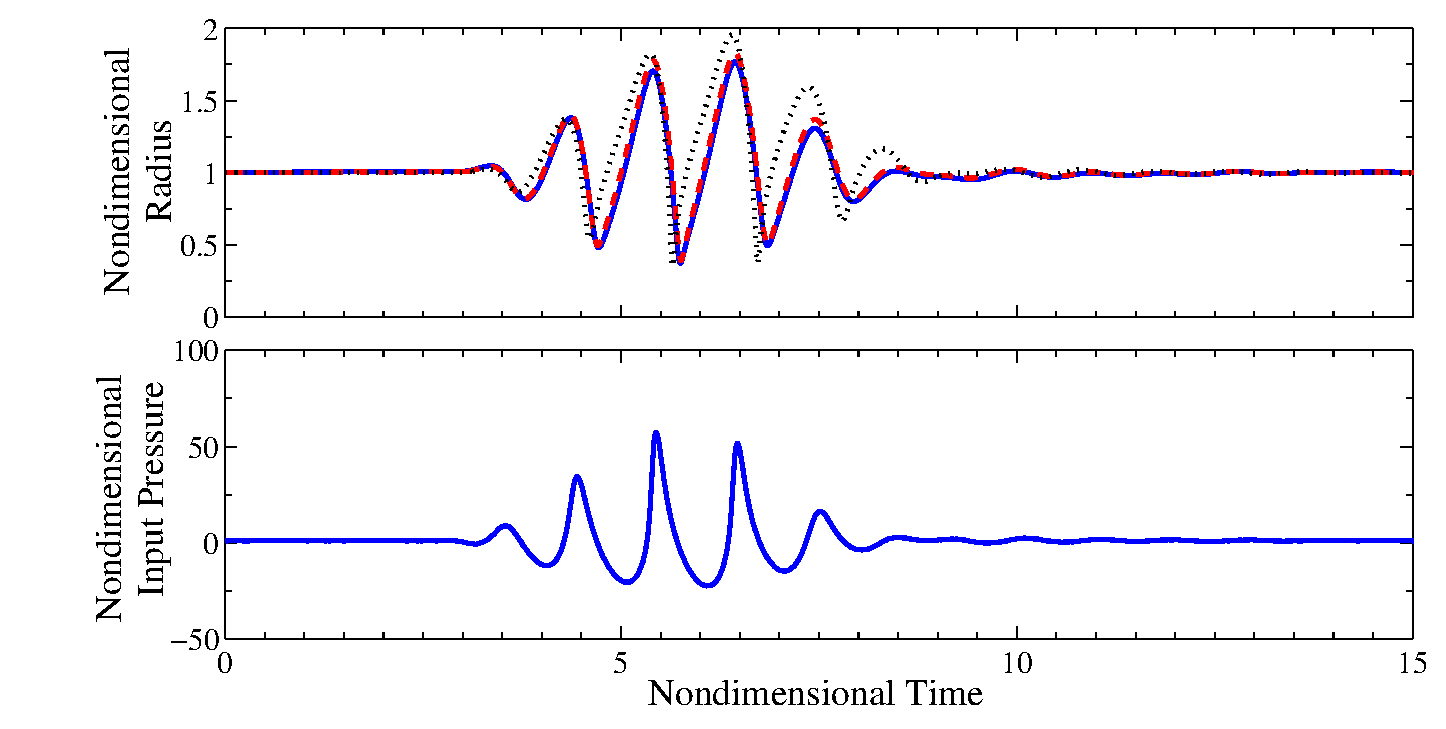
\includegraphics[width=0.66\textwidth]{./figs/bubble_figs/rt_intermediate}%
  \caption{History of the bubble radius (top) and input-pressure
    waveform (bottom) for a moderately nonlinear case (frequency: 3.5 MHz; peak 
    negative pressure: 2.4 MPa). Bioeffects are
    observed here. $R_0=1$ $\mu$m; solid: $G=5$ kPa; dashed: $G=100$ kPa;
    dotted: $G=1$ MPa.}
  \label{figure:sample_bubble_intermediate}
\end{figure}

\begin{figure}
  \centering \includegraphics[width=0.66\textwidth]{./figs/bubble_figs/rt_nonlinear}
  \caption{History of the bubble radius (top) and input-pressure
    waveform (bottom) for a highly nonlinear case (frequency: 
    7.5 MHz; peak negative pressure: 6.0 MPa). Bioeffects are observed
    here. $R_0=1$ $\mu$m; solid: $G=5$ kPa; dashed: $G=100$ kPa; dotted: $G=1$ MPa.}
  \label{figure:sample_bubble_nonlinear}
\end{figure}

In the results of the following sections, the maximum dimensionless radius,
$R_{max}$, and dimensional bubble temperature at collapse, $T_{max}$, obtained
using the ideal gas law, are determined by recording their largest
value over the simulation. These quantities are compared to the
inertial cavitation thresholds used by \cite{Apfel1991} and
\cite{Yang2005}: $R_{max}=2$ and $T_{max}=5000$ K. The dependence
of the bubble dynamics on the pulse amplitude, initial
bubble size (\emph{i.e.}, UCA size distribution), 
pulse frequency, and tissue properties are considered
individually. 



\subsection{Dependence on the Pulse Amplitude}

Given the strong dependence of the MI on the rarefactional pressure
amplitude, the influence of the pulse amplitude on the bubble dynamics
is first evaluated. Fig.~\ref{figure:amplitude} shows the dimensionless
maximum radius as a function of rarefactional pressure
amplitude. Initial bubble radii ranging between 0.1--2.0 $\mu$m are
shown, as well as different frequencies. The open symbols denote
cases where bioeffects did not occur, while the filled symbols denote
the occurrence of bioeffects.

\begin{figure}[t]
  \includegraphics[width=\columnwidth]{./figs/bubble_figs/rstarmax_pm}
  \caption{(color online) Dependence of the dimensionless maximum bubble radius on
    the peak negative pressure for $G=100$ kPa.  Empty symbols: no
    bioeffects; filled symbols: bioeffects. Pentagrams: 0.1 $\mu$m; circles:
    0.5 $\mu$m; squares: 1 $\mu$m; diamonds: 2 $\mu$m; frequency: 1.5 - 7.5 MHz. }
  \label{figure:amplitude}
\end{figure}

The results show that the bubble dynamics, through the maximum radius,
scale with the pulse amplitude. Although the results do not collapse fully
onto a line, a general trend is discernible. At low amplitude, the increase in
the maximum radius is approximately linear; beyond some amplitude, the bubble undergoes
nonlinear oscillations, thus explaining the different depenced and larger spread. 
These results are consistent with the plots shown in 
Figs.~\ref{figure:sample_bubble_linear}-\ref{figure:sample_bubble_nonlinear}.
Over a broad range of amplitudes, the
occurrence of bioeffects has little correlation with pulse amplitude
alone: at a given amplitude, bioeffects may be observed or not,
depending on the bubble size and pulse frequency.  Only at very large
pressure amplitudes (PRPA $>$ 4.20 MPa) are bioeffects systematically observed regardless of the
bubble size and pulse frequency. This behavior is not surprising, since at
these amplitudes the bubble response is expected to be highly
nonlinear. Conversely, at low amplitudes (PRPA $<$ 0.97 MPa), the oscillations are 
linear and no bioeffects are observed, regardless of
bubble size and pulse frequency. In this latter case, most bubbles
whose $R_{max}/R_o$ is below two do not exhibit bioeffects; however,
this behavior depends on the value of elasticity, as shown in \S
\ref{section:tissue_properties}.  Although not shown here for conciseness,
similar results are obtained for peak positive pressure.


Similarly, the criterion $T_{max} > 5000$ K is not achieved with perfluoropropane.
As shown in Fig.~\ref{figure:gascontents}, the observed temperatures for
PFP are far below this value, though the results for air approach it. This
result is expected since the criterion was determined for air, which
has a larger specific heats ratio ($\gamma_{air}=1.4$) than
PFP ($\gamma= 1.13$). The specific heats ratio appears in
the internal gas pressure term in Eq.~\ref{eq:bubble_pressure}; its
effect on the bubble dynamics is minor if the minimum radius is not
very small, as in Fig.~\ref{figure:gascontents}. Still, since the
adiabatic relationships for an ideal gas are used, the temperature is
significantly affected by the different specific heats ratio. Hence,
even though the bubble dynamics are not strongly affected by the
specific heats ratio, the maximum temperature is.

\begin{figure*}[t]
  \begin{subfigure}[b]{0.47\textwidth}
  \includegraphics[width=\textwidth]{./figs/bubble_figs/pfpair}
  \caption{History of the bubble radius for PFP (solid) and air
    (dashed). $R_0=1$ $\mu$m; frequency: 3.5 MHz; peak negative
    pressure: 3.3 MPa}
\end{subfigure}
  \begin{subfigure}[b]{0.47\textwidth}
    \includegraphics[width=\textwidth]{./figs/bubble_figs/tmaxpfpair} 
    \caption{Maximum temperature for PFP (circles) and air (squares). $R_0=0.1-2$ $\mu$m; frequency: 1.5 - 7.5 MHz.}
  \end{subfigure}
  \caption{(color online) Dependence of the bubble dynamics on the gas contents ($G=100$ kPa).}
  \label{figure:gascontents}
\end{figure*}

% \begin{figure*}[t]
%   \subfigure[History of the bubble radius for PFP (solid) 
%     and air (dashed). $R_0=1$ $\mu$m; frequency: 3.5 MHz; peak negative pressure: 3.3 MPa]{
%   \includegraphics[width=0.47\textwidth]{./figs/bubble_figs/pfpair} }
%   \subfigure[Maximum temperature for PFP (circles) and air (squares). $R_0=0.1-2$ $\mu$m; frequency: 1.5 - 7.5 MHz. ]{
%   \includegraphics[width=0.47\textwidth]{./figs/bubble_figs/tmaxpfpair} }
%   \caption{(color online) Dependence of the bubble dynamics on the gas contents
%   ($G=100$ kPa).}
%   \label{figure:gascontents}
% \end{figure*}






\subsection{Dependence on the Initial (Equilibrium) Bubble Radius}

In the experiment, the size distribution of the UCAs is not known
exactly. It is desirable to know whether the observed bioeffects are
caused by all bubbles responding to the ultrasound, or whether a
specific size is more likely to be responsible at the bioeffects
threshold. To answer this question, for each experimental frequency,
bubbles of different radii ranging from 0.1--2 $\mu$m are subjected to
the pressure waveform corresponding to the bioeffects threshold
amplitude. It should be noted that varying the equilibrium radius
changes the non-dimensional parameters. Fig.~\ref{figure:size} shows the maximum dimensionless
radius, for both water (zero elasticity) and tissue (finite
elasticity, $G=100$ kPa), for the amplitude at which bioeffects are
first observed at a given frequency.

\begin{figure}[t]
    \includegraphics[width=\columnwidth]{./figs/bubble_figs/rstarmax_r0}
    \caption{(color online) Dependence of the dimensionless maximum bubble radius on
      the initial bubble size for the amplitude at which bioeffects
      are first observed, at a given frequency, for $G=100$ kPa. Empty
      symbols: water; filled symbols: tissue. Circles: 1.50 MHz; squares:
      2.25 MHz; diamonds: 3.50 MHz; pentagrams: 5.00 MHz; hexagrams: 7.50 MHz.}
    \label{figure:size}
\end{figure}

Excluding the smallest size, the bubble response in tissue is monotone
and changes little for a given frequency; there is no initial size
that consistently leads to a dramatic response. The somewhat erratic
behavior of the small bubbles may imply that such sizes are not
present in UCA concentrations. On the other hand, the behavior is more
irregular for water, particularly at small radii: for a given
frequency, there is an optimal size that exhibits the largest
response; these variations are much larger than for tissue.  








\subsection{Dependence on the Pulse Frequency}

The dependence of the bubble response on the pulse frequency is
considered in this section.  Fig.~\ref{figure:freq} shows the maximum
dimensionless and dimensional radius for all initial bubble sizes and
amplitudes vs. frequency. The square symbols denote cases in which
bioeffects were observed in the experiments, while the circular symbols
represent no bioeffects. The initial bubble sizes are not
discriminated here for simplicity.


\begin{figure*}[t]
  \begin{subfigure}[b]{0.47\textwidth}
    \includegraphics[width=\textwidth]{./figs/bubble_figs/rstarmax_f}  
    \caption{Dimensionless maximum bubble radius.}
  \end{subfigure}

  \begin{subfigure}[b]{0.47\textwidth}
    \includegraphics[width=0.47\textwidth]{./figs/bubble_figs/rmax_f}      
    \caption{Dimensional maximum bubble radius.}
  \end{subfigure}
  \caption{(color online) Dependence of the bubble dynamics on the frequency for
    $G=100$ kPa. $R_0=0.1-2$ $\mu$m; empty circles: no bioeffects; squares:
    bioeffects.}
  \label{figure:freq}
\end{figure*}

With the exception of a few outliers, a clear separation between cases
for which bioeffects did and did not occur is observed; in other
words, the bioeffects threshold has a strong dependence on the
frequency. The trend appears to be approximately linear with
frequency. Large growth may be achieved with no evident bioeffects,
especially at high frequencies. The quantity $R_{max}$ is a
measure of cavitation collapse, since it is related to the available
energy of the bubble. Thus, the present results indicate that
cavitation collapse is expected to play an important role regarding
bioeffects, although the precise mechanism cannot be inferred.  Again,
the existing criteria for inertial cavitation thresholds are
frequency-independent and do not correlate well with the bioeffects
threshold, which clearly shows a strong dependence on frequency.

Another hypothesis is that bubble growth may be responsible for
capillary breaching. However, the plot of the dimensional maximum radius vs. frequency does
not show systematic bioeffects beyond a certain size, \emph{e.g.},
some capillary diameter. Thus, growth is not the sole mechanism by
which bioeffects occur. However, the data remains inconclusive,
due to the inability to identify the cases in which cavitation
collapse is the dominant effect.






\subsection{Dependence on the Tissue Properties}
\label{section:tissue_properties}

As suggested in
Figs.~\ref{figure:sample_bubble_linear}-\ref{figure:sample_bubble_nonlinear},
the bubble dynamics are sensitive to the tissue properties,
specifically the elasticity. However, different types of tissue may
have very different properties. Many of the measurements of tissue elasticity are made
\emph{in vitro}, and depend strongly on tissue preparation, storage,
and degradation as well as method of measurement.  Consequently it is
possible that these measurements do not accurately represent the
current behavior.  To explore the effect of the elasticity on the
results and the correlation to bioeffects, Fig.~\ref{figure:freq_tissue}
shows the maximum dimensionless radius for all initial bubble sizes
and amplitudes vs. frequency for $G=5$ kPa and $G=1$ MPa. Although
seemingly high, the latter elasticity is chosen to match the work of
\cite{Yang2005}.

\begin{figure*}[t]
  \begin{subfigure}[b]{0.47\textwidth}
    \includegraphics[width=\textwidth]{./figs/bubble_figs/rstarmax_f_ca=20}
    \caption{$G=5$ kPa.}
  \end{subfigure}

  \begin{subfigure}[b]{0.47\textwidth}
    \includegraphics[width=\textwidth]{./figs/bubble_figs/rstarmax_f_ca=0,1}    
    \caption{$G=1$ MPa.}
  \end{subfigure}
  \caption{(color online) Dependence of the dimensionless maximum bubble radius on
     the frequency. $R_0=0.1-2$ $\mu$m; empty circles: no bioeffects; squares:
     bioeffects.}
  \label{figure:freq_tissue}
\end{figure*}

% \begin{figure*}[t]
%   \subfigure[$G=5$ kPa.]{
%     \includegraphics[width=0.47\textwidth]{./figs/bubble_figs/rstarmax_f_ca=20}
%   }
%   \subfigure[$G=1$ MPa.]{
%     \includegraphics[width=0.47\textwidth]{./figs/bubble_figs/rstarmax_f_ca=0,1}    
%   }
%    \caption{(color online) Dependence of the dimensionless maximum bubble radius on
%      the frequency. $R_0=0.1-2$ $\mu$m; empty circles: no bioeffects; squares:
%      bioeffects.}
%   \label{figure:freq_tissue}
% \end{figure*}

The bubble dynamics and correlation to bioeffects significantly change
when reducing the elasticity. For a value of 5 kPa, the discrimination
is no longer clear. The bubble dynamics are closer to the behavior in
water, such that different sizes may have dramatically different
responses to the same waveform, as explained previously. On the other
hand, the stiffer medium ($G=1$ MPa) shows an even sharper
demarcation, which again appears to be approximately linear. Given the
sensitivity of the results on the elasticity, it is clear that more
precise \emph{in vivo} data is required for elasticities of tissues at the
relevant strain rates. 

Although not shown here, the type of
viscoelastic model significantly affects the bubble dynamics
\cite[]{Johnsen2012}. For instance, a standard linear solid
model, which includes stress relaxation in addition to elasticity, leads 
to very different maximum
radii and oscillation properties (frequency and damping).  For
large relaxation times, elasticity variations become negligible.




\section{Conclusions}
\label{sec:usbe_bubble_conclusions}

In the present work, a numerical model is used
to investigate experimentally observed bioeffects as a result of
contrast-enhanced ultrasound. This work is unique in its 
combination of experimental results and numerical modeling.
For the experimentally generated input
pressure waveforms, it is known which of these triggered bioeffects,
and from the numerical model we obtained calculated values for
the dimensionless maximum radius and dimensional maximum temperature for each of these cases.  By comparing the
results of this study to previously established inertial cavitation
thresholds used by \cite{Apfel1991} and \cite{Yang2005},
$T_{max}=5000$ K and $R_{max}=2$, it would appear that the inertial
cavitation threshold does not play a role in determining the bioeffects
threshold.  However, it is unlikely that the inertial cavitation
threshold is irrelevant. Instead, it is far more probable that these
thresholds are not defined appropriately for cavitation in a
viscoelastic medium, such as soft tissue. This work suggests the need for
further experimental and numerical studies of cavitation in viscoelastic media.

The present work shows a strong correlation between cavitation dynamics and bioeffects
when considering the pulse frequency.
From the plot of maximum
dimensionless radius vs. frequency, there is a clear separation
between when bioeffects do and do not occur, and based on these
results it appears that the frequency of the input pressure waveforms
is of key importance to the definition of a bioeffect threshold, and
likely the inertial cavitation threshold as well. 

The present work shows that the elasticity of tissue significantly
affects the bubble dynamics. This finding is perhaps not completely
unexpected given that bubble dynamics are known to strongly depend
on viscoelastic properties and model. The present study shows the need
for more accurate measurements of material properties and for
determining appropriate constitutive models for soft tissue,
particularly at high strain rates. Finally, although the present work
suggests that inertial cavitation collapse plays an important role with respect
to bioeffects, it does not shed light on the exact mechanism,
\emph{e.g.}, shock emission upon collapse, growth beyond a given size,
high temperatures generating free radicals, re-entrant jets in
non-spherical collapse, etc.  In future work we plan on investigating 
this injury mechanism by conducting direct simulations of
the full equations of motion for bubble dynamics in a viscoelastic medium.


%%% Local Variables:
%%% mode: latex
%%% TeX-master: t
%%% End:

\acresetall
% %
% Acoustically-driven gas-liquid interfaces


% US Bioeffects: DUS-induced Lung Hehorrage work
\chapter{Growth of liquid-gas interfacial perturbations driven by acoustic waves} \label{ch:usbe_lung}%
\input{./content/chapters/usbe_lung_paper_chapter}


\acresetall
\chapter{Pulsed ultrasound-induced stresses and strains at gas-liquid interfaces} \label{ch:usbe_lung_bio}%
In Chapter \ref{ch:usbe_lung} we introduced the problem of
\ac{DUS}-induced lung hemorrhage, however, the focus was on the
fundamental physical problem of an acoustically driven gas-liquid
interface, such as those of the alveoli. In this chapter, we aim to
extend that work to increase its relevance to \ac{DUS} of the
lung. Here, we hypothesize that real \ac{DUS} waves may be capable of
generating sufficient baroclinic vorticity at alveolar interfaces in
the lung to drive deformation and hemorrhage. To investigate this
hypothesis we again model the alveolus as a perturbed water-air
interface and examine the dynamics when driven by ultrasound pulses
with clinically relevant parameters. We compare the interface
evolution to that expected of a vorticity driven interface based on
the work of Chapter \ref{ch:usbe_lung}. Furthermore, we infer the
viscous stress and calculate the approximate strain at the interface
and compare computed values to expected alveolar damage thresholds,
based on previous published research.

\section{Abstract}
\ac{DUS}-induced lung hemorrhage in mammals is the only known
biological effect of non-contrast diagnostic ultrasound. Despite years
of study, the underlying physical mechanism remains unknown. In this
work we model the interaction between an ultrasound pulse and an
alveolus as an acoustic wave in water propagating toward a water-air
interface. To capture the alveolar surface roughness the interface
contains a single-mode sinusoidal perturbation, representing the
alveolar surface roughness, of variable initial amplitudes equal to 3,
10, and 30\% of the perturbation wavelength, which represents the
alveolar diameter. By solving the Euler equations of fluid motion we
study the evolution of the interface for 1.5 MHz ultrasound with peak
amplitudes of 1.0, 2.5, and 5.0 MPa. The interface is observed to
continue deforming long after the passage of the wave. Interfacial
strains of up to 38\% after 288 $\mu$s. Viscous stresses are estimated
and maximum amplitudes are found to be on the order of $10$ Pa. For a
10 MPa pulse, interface perturbation amplitudes are shown to grow
approximately as $t^{3/5}$, which is expected of vorticity-driven
growth based on the work of Chapter \ref{ch:usbe_lung}.

\section{Introduction}
Lung \ac{US} has become a common tool for imaging and diagnostics in
critical and point-of-care situations and its use is growing
\citep{Lichtenstein2009}. Currently, \ac{PCH} is the only biological
effect known to occur in mammals as a result of non-contrast
diagnostic ultrasound. It has been shown to occur under clinically
acceptable parameters with \ac{MI}$\leq1.9$ \citep{FDA1997} and peak
pressures as low as $1.0$ MPa \citep{Dalecki1997}. The physical
mechanism underlying this damage is still not well understood. While
the occurrence of hemorrhage as a result of diagnostic lung \ac{US}
has not been directly studied in human lungs for obvious ethical
reasons, an understanding of the underlying cause is important for the
development of evidence-based safety guidelines and regulations.

\ac{US}-induced \ac{LH} is not a new problem. It was first discovered
in mice over twenty years ago \citep{Child1990}. And since then, there
has been considerable work to progress our understanding. Much of this
previous research has primarily aimed at three specific ends: (1)
investigating the physical damage mechanism causing the hemorrhage;
(2) determining the dependence of damage characteristics and
bioeffects thresholds on the \ac{US} properties; and (3) determining
the dependence of damage characteristics and thresholds on the
characteristics of the \ac{US} subject. This study aims to contribute
to the first of these areas: we aim to estimate the potential stresses
and strains imparted by a single ultrasound pulse on a perturbed
liquid-gas interface, similar to that of a single alveolus. To do this
we will extend the computational fluids model of an \ac{US}-driven
alveolus developed in Chapter \ref{ch:usbe_lung} to include \ac{US}
pulse-like waveforms and interface geometries with larger perturbation
amplitudes than previously considered, which are more representative
of physical alveoli.

In Chapters \ref{ch:Introduction} and \ref{ch:usbe_lung}, a portion of
the body of past research into the physical mechanisms of \ac{DUS} was
reviewed, so only a brief summary is provided
here. \ac{US}-induced pulmonary hemorrhage is characterized by alveoli
filling with blood as well as plasma proteins and erythrocytes
\citep{Miller2016a,Penney1993a}. Alveolar edema or frank hemorrhage
has also been shown to occur as a result of mechanical stress failure
of the alveolar membrane induced by over pressure
\citep{West1991}. The cause of \ac{DUS}-induced hemorrhage in the
lungs appears mechanical in nature and thermal mechanisms appear
unlikely to cause the observed damage \citep{Zachary2006,
  Dalecki2004}. Cavitation, acoustic radiation force, resonance, and
acoustic fountaining or atomization have all been studied as possible
mechanical damage mechanisms for \ac{DUS}-induced \ac{LH}
\citep{Holland1996,Miller2016a,Jabaraj2012,Jabaraj2013,Jabaraj2013a,Tjan2007,Simon2012}.
Experimental results suggest that the most common mechanical
ultrasound bioeffect mechanism, cavitation, is unlikely, and for
reasons detailed in the previous chapters, none of the remaining
mechanisms completely explains the damage \citep{OBrien2000,
  Raeman1996, Miller2016a}.

Research investigating the dependence of \ac{US}-induced \ac{LH} on
the characteristics of the \ac{US} subject has considered species,
age, physiological development, and pulmonary state of the \ac{US}
subject.  Within mammals, the occurrence of \ac{DUS}-induced \ac{LH}
has been observed to be largely species-indiscriminate and has been
found to occur in mice, pigs, rats, rabbits, and monkeys
\citep{Baggs1996, Child1990, Dalecki1997, Frizzell1994, Frizzell2003,
  Harrison1995, Holland1996, Kramer2001, OBrien1997a, OBrien2001b,
  OBrien2003a, OBrien2005, OBrien2000, OBrien2001a, Penney1993a,
  Raeman1993, Raeman1996, Tarantal1994a, Zachary1995a, Zachary2001a,
  Zachary2001}. \cite{Dalecki1997} subjected neonatal, juvenile, and
adult mice to pulsed ultrasound of the lung and observed that while
hemorrhage thresholds were similar in all mice, the degree of
hemorrhage was much greater in the adult mice than in the younger
subjects. Similarly, \cite{OBrien2003a}, studied the age dependence of
hemorrhage in pigs, and found that older pigs had a significantly
lower hemorrhage thresholds than juvenile and middle-aged pigs. In an
unexpected result, the study also found that if one lung was exposed
to \ac{US} and the pig was then rolled over and the second lung
exposed, the hemorrhage threshold in the second lung was substantially
lower than in the first. To study the dependence of hemorrhage on the
impedance boundary condition at the lung’s pleural surface,
\cite{OBrien2002a} subjected rats with variable degrees of lung
inflation to 3.1 MHz pulsed \ac{US} with \ac{PRPA} $=8.6, ~16$ MPa. It was
found that deflated lungs, which had less impedance mismatch with
their surroundings, were more easily damaged than partially deflated
lungs, which were more easily damaged than inflated lungs. While no
direct experimentation has been performed on humans, for obvious
ethical reasons, \cite{Meltzer1998} found that transesophageal
echocardiography with similar \ac{US} parameters to those causing lung
hemorrhage in animal studies ($3.1$ MHz, \ac{PRPA}$= 2.4$ MPa) did not
lead to visible hemorrhage on the surface of the lung. While
\ac{DUS}-induced \ac{LH} has not been shown to occur in humans, its
occurrence in a wide variety of mammals under diagnostically relevant
conditions suggests a need for further investigation.

The body of research investigating the dependence of lung hemorrhage
on \ac{US} properties is extensive and has investigated the dependence
of hemorrhage occurrence and severity on a wide variety \ac{US}
parameters. \cite{Zachary1995a} used continuous-wave and pulsed-wave
\ac{US} in mice, rabbits, and pigs, and found that continuous- and
pulsed-wave-induced lesions appear macroscopically similar, but
differed microscopically. Hemorrhage induced by continuous wave
\ac{US} consisted primarily of plasma and contained some cells,
whereas pulsed-wave induced hemorrhage was composed mostly of cells
and contained little plasma. \cite{Raeman1996} subjected mice to 2.3
MHz pulsed \ac{US} with peak pressures up to 3 MPa and varying
exposure time and found that while threshold amplitudes appeared
insensitive to exposure time, suprathreshold damage increased with
increasing exposure. In a review of previous work, \cite{Miller2016a}
indicated that previously observed differences in bioeffects
thresholds between studies may be attributable to exposure duration
differences. \cite{OBrien2001} investigated the effects of \ac{US}
beamwidth and found that for rats subjected to 2.8 and 5.6 MHz
ultrasound, incidence, surface area, and volume of hemorrhage
increased with increasing beamwidth. It was noted that lung hemorrhage
is perhaps the only known beamwidth-dependent mechanical bioeffect of
\ac{US}. \cite{OBrien2003c} found evidence that increasing \ac{US}
pulse duration decreases the \acp{PRPA} threshold associated with a
5\% likelihood of lung hemorrhage in rats subjected to 2.8 MHz
ultrasound with peak amplitudes ranging from 4-9 MPa. Given that the
dependencies of bioeffects on waveform amplitude and frequency are not
fully understood, we consider the dependence of the alveolar wall
dynamics on acoustic wave amplitude.

Separately, the structure, mechanical behavior, and failure properties
of alveoli have been studied extensively and are of particular
interest to the present work. The alveoli can be thought of as a
network of openly connected, air-filled saccules with distinctly
irregular surfaces. Past research suggests that alveolar size is
species dependent \citep{Faffe2002}. While alveoli are not perfect
spheres, their mean diameters range from tens to hundreds of microns,
with reported values of 45 $\mu$m in mice and 200 $\mu$m in adult
humans \citep{Knust2008,Ochs2004}. The septa separating adjacent
alveoli are nearly planar structures that contain several tissue
layers and are coated with a thin layer of liquid surfactant
\citep{Gil1979,Reifenrath1975,Perlman2014}. Within the alveolar septa
surrounding the alveoli, are the pulmonary capillaries, a sheet-like
web which is almost completely unsupported by surrounding tissue
\citep{West1991}. Separating the blood from the air is a multi-layer
wall of tissues, $0.2$ - $0.3\mu$m thick, referred to as the blood-gas
or blood-air barrier \citep{West2000}. \cite{West1991} raised the
pulmonary capillary pressure of anesthetized rabbits and observed
consistent stress failure of the capillary and alveolar epithelium for
transmural at or above $40$ mmHg ($5.3$ kPa). It was observed that
failure corresponded to approximately $25$ mN/m wall tension in the
capillaries, and noted that ``this tension is small, comparable with
the tension in the alveolar wall associated with elastic recoil.''
The capillary wall stress at failure was calculated to be
approximately $8$ kPa. Alveolar wall strain has also been studied and
linear, alveolar strain due to normal tidal breathing is reported to
range from $0$ -- $5$\% for humans \citep{Roan2011}. \cite{Belete2010}
found that when subjected to cyclical linear stretch at 0.5 Hz for 30
minutes, rat alveolar epithelial cells experiencing linear strains of
$8\%$ or greater were frequently damaged, whereas those experiencing
strains of $3$ -- $6\%$ were often undamaged.

This work is the first to use a fully nonlinear, Euler-based
computational fluids approach to study the dynamics of an alveolus
driven by a single ultrasound pulse. Extending the alveolar model of
Chapter \ref{ch:usbe_lung}, we perform numerical experiments to
simulate the dynamics of gas-liquid interfaces driven by ultrasound
pulse waveforms within the clinically relevant range. Using simple
models, we approximate the linear interfacial strain and infer viscous
stress at the interface, which we compare to alveolar failure criteria
from relevant literature. Additionally, we compare the interface
evolution to that expected of a vorticity-driven growth of interfacial
perturbation, based on our past work \citep{Patterson2017,Patterson2017b}.

%%%%%%%%%%%%%%%%%%%%%%%%%%%%%%% 
\section{Methods}
Much of the basic problem setup and computational framework detailed
in Chapter \ref{ch:usbe_lung} are reused here. In this section we
briefly summarize the model and then focus specifically on three
specific areas where changes have been to better suit our focus on
\ac{DUS}-induced \ac{LH}: (1) problem geometry, (2) incoming waveform,
(3) calculation of stress and strain.

v% \subsection{Summary of the model problem}
% We consider the problem of a single outermost alveolus driven by a
% single \ac{DUS} pulse, initially trAveling In adjacent to soft
% tissue. We model this problem as an \ac{US} wave in water impinging
% upon a sinusoidally perturbed air interface. This is consistent with
% the idea of alveoli as a network of openly connected, air-filled
% saccules with distinctly irregular surfaces. As such they have no true
% ``diameter'', but as past research suggests that their size appear to
% be species dependent \citep{Faffe2002}, we restrict our model and
% consider only an adult human alveolus which has a characteristic mean
% diameter of 200 $\mu$m \citep{Ochs2004}.

In the previous chapter, we simulated trapezoidal acoustic waves
impinging upon a nearly planar interface with a sinusoidal
perturbation. The width of the domain represents a single alveolar
diameter, $\ell=200 \mu$m in adult humans \citep{Ochs2004}, which is
also the wavelength of the perturbation. The initial perturbation
amplitude used $a_0=0.03\ell$, implies a nearly flat alveolar surface,
which is not always the case, as can be seen in the histological cross
section of alveoli shown in Figure \ref{fig:alveolar_histology}. To
account for the variety of geometries in alveolar tissue, many of
which are not particularly flat. A typical surface radius of curvature
for a human alveolus has been reported as $109~\mu$m
\citep{Mercer1994}. We will now consider perturbation amplitudes of
$a_0=0.03\ell, 0.10\ell$ and $a_0=0.30\ell$. We acknowledge that this
does not capture the true range of cross-sectional alveolar
geometries. However, this simplified geometry, necessitated by
computational constraints, will allow for the generalization of the
conclusions of this work broadly to relevant geometries.
\begin{figure}%
  \begin{subfigure}{0.45\textwidth}
    \centering%
    \includegraphics[width=\textwidth]{./figs/lung_figs/alveolar_sac}%
  \end{subfigure}
  ~
  \begin{subfigure}{0.5\textwidth}
    \begin{tikzpicture}%
      \node[anchor=south west,inner sep=0] (image) at (0,0) {
        \includegraphics[width=\textwidth]{./figs/lung_figs/lung_surface_alveoli}
      };%
      \begin{scope}[x={(image.south east)},y={(image.north west)}]%
        \node[left] at (1.0,0.95) {Soft tissue};%
        \node[left] at (1.0,0.38) {Lung surface};%
        \node[left] at (0.95,0.08) {\colorbox{gray!40}{Alveoli}};%
      \end{scope}%
      %
      \node[anchor=south west,inner sep=0] (image_wave) at (0.0,2.6) {
      \def\svgwidth{0.425\textwidth}\import{./figs/lung_figs/}{wave_only.pdf_tex}};%
      \draw[very thick] (1.3,1.7) -- (2.2,1.7) -- (2.2,2.5) -- (1.3,2.5) -- (1.3, 1.7); %
    \end{tikzpicture}%
  \end{subfigure}
  \caption[A histological cross section of alveoli.]{A histological
    cross section of alveoli (Left). A schematic of ultrasound
    impinging upon the lung surface and alveoli, from the surrounding
    soft tissue (Right). A black box surrounds an alveolar surface,
    which schematically illustrates the physical problem upon which
    the initial condition is created.[Alveolar cross section adapted
    from work by Jpogi [CC BY-SA 4.0
    (http://creativecommons.org/licenses/by-sa/4.0), via Wikimedia
    Commons]}%
  \label{fig:alveolar_histology}
\end{figure}%
% 
The diagnostic ultrasound pulse waveform, as illustrated in the time
domain in Figure \ref{fig:p0_ultrasound} is modeled as a sinusoidal
carrier wave of amplitude $p_a$ and frequency $f$ modulated by a
Gaussian Envelope, and as such that the initial pressure condition can
be described as,
\begin{align}
  p(y_f,t=0) = p_a\sin{\left(2\pi f\frac{y_f-L}{c}\right)}\exp{\left(-\frac{\left(\left[y_f-L/2\right]c\right)^2}{FWHM/\left(2\sqrt{2\ln{\left(2\right)}} \right)}\right)},%
\end{align}
where $y_f = y - 11a_0$ is the $y$-location, relative to the initial
location of the wave leading end. The carrier wavelength
$\lambda=c_{water}/f$ and the full width of the Gaussian envelope at
half of the maximum amplitude, or $FWHM$, are designed to scale
appropriately with respect to the alveolar length scale
$\ell=200~\mu$m. Here, we choose design parameters of
$f\approx 1.25 c / 2\pi \ell$ and $FWHM=15\ell$ such that the
corresponding center frequency is approximately $f=1.5$ MHz and
$FWHM=3$ mm. Accordingly, the pulse length $L=45\ell$ is defined such
that the pulse duration is approximately $6~\mu$s. In implementation
$L$ is the length of the computational domain, over which the wave is
defined to exist (i.e., pressure is set to ambient outside the wave
region, effectively truncating the ends of the Gaussian
envelope). This waveform is an analytical approximation of a true
\ac{DUS} pulse, which allows us to manipulate the parameters of
interest. %
\begin{figure}
  \centering \def\svgwidth{0.5\textwidth}
  \import{./figs/lung_figs/}{p0_vs_t_us_general.pdf_tex}%
  \caption[Ultrasound pulse waveform]{Ultrasound pulse waveform}
  \label{fig:p0_ultrasound}%
\end{figure}%

\subsection{Stress and strain at the alveolar interface}%
\label{subsec:usbe_lung_bio_stress_strain}
As previously mentioned, among the tissue layers surrounding the
alveoli are the pulmonary capillaries, a sheet-like, blood-filled web,
almost completely unsupported by surrounding tissue
\citep{West1991}. It is the hemorrhage of these capillaries that
interests us, and thus, to interpret the results of the numerical
experiments in the context of \ac{DUS}-induced lung hemorrhage, we
will calculate the linear strain and infer the viscous stress at the
liquid-gas interface, which represents the alveolar septa, where these
capillaries lie. We aim to compare the calculated stresses and strains
to relevant injury criteria. We note that from the available strain
and strain rate data, it would be possible to infer a total
viscoelastic stress at the interface if a constitutive model were
known. However, constitutive models appropriate to this work do not
appear available at this time and the development of such models would
require experiments far beyond the scope of this work.%
\begin{comment}
  For sake of justification of the model, a simple model for
  estimating the order of magnitude of the involved elastic forces can
  be found in \ref{app:lung_elastic}
\end{comment}

\paragraph*{Calculation of the viscous stress}
Viscous stresses resist motion of the flow, however since the Euler
equations, which are inherently inviscid, are solved, we aim to infer
the viscous stress resulting from the interfacial motion and
deformation. We do this because, while the justifications in Chapter
\ref{ch:usbe_lung} suggest that flow dynamics can be reasonably
approximated by neglecting viscosity an understanding of the
approximate viscous stress associated with \ac{DUS} is necessary to
understand the results in the context of alveolar injury. To do this
we infer the viscosity at each point in space and time as $\mu(x,y,t)$
based on the physical properties of air and water, and the volume
fraction of water $\alpha(x,y,t)$ given that
$\mu = \alpha\mu_{water} + (1-\alpha)\mu_{air}$. The shear stress in a
two-dimensional, Newtonian flow is calculated using the computed
viscosity field and the velocity gradients as
\begin{align}
  \tau_{xy}(x,y,t) = \mu\left(\frac{\partial u}{\partial y}+ \frac{\partial v}{\partial x}\right),
\end{align}
where $u$ and $v$ represent the $x$- and $y$-components of the
velocity. The maximum viscous stress amplitude is extracted from the
field at each point in time from our simulations.
% 
\begin{comment}
  \begin{align}%
    \tau_{ij}=\mu%
    \begin{bmatrix}%
      0 & \frac{\partial u}{\partial y}+\frac{\partial v}{\partial x}\\%
      \frac{\partial v}{\partial x}+\frac{\partial u}{\partial y} & 0%
    \end{bmatrix}%
  \end{align},
\end{comment}
% 
\paragraph*{Calculation of the interface strain}
The linear interfacial strain is calculated as
\begin{align}%
  \label{eq:linear_strain}%
  \varepsilon = \frac{s(t) - s_0}{s_0}
\end{align}
where $s(t)$ is the arc length of the interface, which is initially
$s_0=s(0)$.  While some of the large deformations we observe in our
results may actually be out of the realm of finite strain, we choose
this metric, which is consistent with previous alveolar strain
calculations in the literature. For example, \cite{Roan2011} used the
relative change in alveolar diameters, which is analogous to relative
change in the interface arc length here.
\begin{comment}
  \cite{Perlman2014} combined experimentally measured strains with
  computationally modeled lung stresses to demonstrate that the
  effective Young's moduli of alveolar septa depend on transpulmonary
  pressure. Values range from a minimum of $E_a=12$ kPa in the low
  transpulmonary pressure range of $\approx 0.4$-$0.6$ kPa to a
  maximum $E_a=140$ kPa at a high transpulmonary pressure of range,
  $\approx 1.5$-$2.5$ kPa.
\end{comment}

%%%%%%%%%%%%%%%%%%%%%%%%%%%%%%% 
\section{Results and Discussion}
To accomplish the aims of this study, two sets of numerical
experiments are performed. The first set of experiments is designed to
determine the stresses and strains on a perturbed liquid-gas
interface, driven by clinically relevant ultrasound
pulses. Simulations of interactions between sinusoidally perturbed
water-air interfaces and diagnostic ultrasound pulses are performed
for wave amplitudes of $p_a=1.0$, $2.5$, and $5.0$ MPa and initial
perturbation amplitudes of $a_0=0.03\ell$, $0.10\ell$ and
$0.30\ell$. The second set of experiments is designed to test the
hypothesis that \ac{US} pulses are capable of generating sufficient
baroclinic vorticity at an air-water interface to drive appreciable
interface deformation. For this second set of experiments, which is
described in greater detail in Section
\ref{subsec:vorticity_experiments}, we perform simulations of an
\ac{US} pulse-driven gas-liquid interface, with parameters similar to
those of the baseline trapezoidal wave in Chapter \ref{ch:usbe_lung}
($p_a = 10$ MPa, $a_0 = 0.03\ell$, $L=45\ell$) and compare interface
growth dynamics driven by a \ac{US} pulse to those driven by the
trapezoidal wave of Chapter \ref{ch:usbe_lung}.

\subsection{Qualitative observations of the interface}
To illustrate the evolution of the interface, Figures
\ref{fig:rho_snapshots_A10}, \ref{fig:rho_snapshots_A25}, and
\ref{fig:rho_snapshots_A50} show density contours for pulse amplitudes
of $1.0, 2.5,$ and $5.0$ MPa, respectively, at dimensionless times
$t/(\ell/c)=4.75, 47.5, 475,$ and $2374$. While these dimensionless
quantities are used for comparison of this work to that of Chapter
\ref{ch:usbe_lung}, for the sake of physicality, we will report times
and stresses in this section as dimensional quantities. As such, for
an $\ell = 200~\mu$m alveolar diameter, these dimensionless times
approximately corresponds to dimensional times of $0.6, 6.0, 60,$ and
$290~\mu$s. In each case, subfigures \subref{fig:rho_snapshot_03},
\subref{fig:rho_snapshot_10}, and \subref{fig:rho_snapshot_30}
correspond to initial perturbation amplitudes of
$a_0=0.03\ell, 0.10\ell,$ and $0.30\ell$ respectively; $t = 0.6~ \mu$s
occurs just after the wave first encounters the interface and by
$t= 6.0~ \mu$s the wave has completely passed. For the $p_a = 1.0$ MPa
pulse, the interface remains largely unmoved and undeformed by the
interaction with the wave, even at late times (illustrated in Figure
\ref{fig:rho_snapshots_A10}). For the $p_a = 2.5$ MPa pulse, little
deformation is observed for $a_0 = 0.03\ell$, however at higher
initial amplitudes ($a_0 = 0.10\ell$ and $0.30\ell$), the interface is
clearly deformed at late times and a cusp is observed to form along
the interface at $x/\ell = 0.5$ (illustrated in Figure
\ref{fig:rho_snapshots_A25}). For the $p_a = 5.0$ MPa pulse, obvious
deformation is observed for all considered values of $a_0$
(illustrated in Figure \ref{fig:rho_snapshots_A50}). For
$a_0 = 0.10\ell$ and $0.30\ell$, a spike of heavy fluid with a cusp at
$x = 0.5$ is again observed to form at late times.  For all incoming
waves, the degree of deformation appears to increase with increasing
initial perturbation amplitude $a_0$ and wave amplitude $p_a$. The
observed sharp features, which evolved from an initially smooth
interface perturbation, could potentially lead to stress concentration,
which in alveoli, may lead to hemorrhage.
% 
\definecolor{airgray}{HTML}{DDDDDD}
\begin{figure}
  \vspace*{-0.5cm}
  \centering
  \begin{subfigure}[b]{0.9\textwidth}
    \begin{tikzpicture}%
      \node[anchor=south west,inner sep=0] (image) at (0,0) {
        \includegraphics[width=\textwidth]{./figs/lung_figs/rmawave_1_A10_a03_t500_rho_snapshots_printable}
      };%
      \begin{scope}[x={(image.south east)},y={(image.north west)}]%
        \node[font=\small,right] at (0.06,0.9) {\textcolor{white}{$\rho(x,y)$}};%
        \node[font=\small,right] at (0.7,0.9) {\textcolor{white}{(a) $a_0=0.03\ell$}};%
        \node[font=\small,right] at (0.06,0.14) {\colorbox{airgray}{$t = 0.6~\mu$s}};% t/(\ell c_{air})=1
        \node[font=\small,right] at (0.26,0.14) {\colorbox{airgray}{$t = 6.0~\mu$s\quad}};%t/(\ell c_{air})=10
        \node[font=\small,right] at (0.475,0.14) {\colorbox{airgray}{$t = 60~\mu$s\quad}};%t/(\ell c_{air})=100
        \node[font=\small,right] at (0.685,0.14) {\colorbox{airgray}{$t = 288~\mu$s\quad}};%t/(\ell c_{air})=500
      \end{scope}%  
      % \begin{scope}[x={(image.south east)},y={(image.north west)}]%
      %   \node[font=\small,right] at (0.06,0.9) {\textcolor{white}{$\rho(x,y)$}};%
      %   \node[font=\small,right] at (0.06,0.14) {\colorbox{airgray}{$t = 1 $ ($0.6~\mu$s)}};%
      %   \node[font=\small,right] at (0.26,0.14) {\colorbox{airgray}{$t = 10 $ ($6.0~\mu$s)}};%
      %   \node[font=\small,right] at (0.475,0.14) {\colorbox{airgray}{$t = 100 $ ($60.0~\mu$s)}};%
      %   \node[font=\small,right] at (0.685,0.14) {\colorbox{airgray}{$t = 300 $ ($500.0\mu$s)}};%
      % \end{scope}%  
    \end{tikzpicture}%
    \phantomcaption
    \label{fig:rho_snapshot_03}
    % \caption{\label{fig:rho_snapshot_03} $a_0 = 0.03\ell$}
  \end{subfigure}
  % 
  \begin{subfigure}[b]{0.9\textwidth}
    \begin{tikzpicture}%
      \node[anchor=south west,inner sep=0] (image) at (0,0) {
        \includegraphics[width=\textwidth]{./figs/lung_figs/rmawave_1_A10_a10_t500_rho_snapshots}
      };%
      \begin{scope}[x={(image.south east)},y={(image.north west)}]%
        \node[font=\small,right] at (0.06,0.9) {\textcolor{white}{$\rho(x,y)$}};%
        \node[font=\small,right] at (0.7,0.9) {\textcolor{white}{(b) $a_0=0.10\ell$}};%
        \node[font=\small,right] at (0.06,0.14) {\colorbox{airgray}{$t = 0.6~\mu$s}};% t/(\ell c_{air})=1
        \node[font=\small,right] at (0.26,0.14) {\colorbox{airgray}{$t = 6.0~\mu$s\quad}};%t/(\ell c_{air})=10
        \node[font=\small,right] at (0.475,0.14) {\colorbox{airgray}{$t = 60~\mu$s\quad}};%t/(\ell c_{air})=100
        \node[font=\small,right] at (0.685,0.14) {\colorbox{airgray}{$t = 288~\mu$s\quad}};%t/(\ell c_{air})=500
      \end{scope}%  
    \end{tikzpicture}%
    \phantomcaption
    \label{fig:rho_snapshot_10}
    % \caption{\label{fig:rho_snapshot_10} $a_0 = 0.10\ell$}
  \end{subfigure}
  % 
  \begin{subfigure}[b]{0.9\textwidth}
    \begin{tikzpicture}%
      \node[anchor=south west,inner sep=0] (image) at (0,0) {
        \includegraphics[width=\textwidth]{./figs/lung_figs/rmawave_1_A10_a30_t500_rho_snapshots}
      };%
      \begin{scope}[x={(image.south east)},y={(image.north west)}]%
        \node[font=\small,right] at (0.06,0.9) {\textcolor{white}{$\rho(x,y)$}};%
        \node[font=\small,right] at (0.7,0.9) {\textcolor{white}{(c) $a_0=0.30\ell$}};%
        \node[font=\small,right] at (0.06,0.14) {\colorbox{airgray}{$t = 0.6~\mu$s\quad}};% t/(\ell c_{air})=1
        \node[font=\small,right] at (0.26,0.14) {\colorbox{airgray}{$t = 6.0~\mu$s\quad}};%t/(\ell c_{air})=10
        \node[font=\small,right] at (0.475,0.14) {\colorbox{airgray}{$t = 60~\mu$s\quad}};%t/(\ell c_{air})=100
        \node[font=\small,right] at (0.685,0.14) {\colorbox{airgray}{$t = 288~\mu$s\quad}};%t/(\ell c_{air})=500
      \end{scope}%  
    \end{tikzpicture}%
    \phantomcaption
    \label{fig:rho_snapshot_30}
    % \caption{\label{fig:rho_snapshot_30} $a_0 = 0.30\ell$}
  \end{subfigure}
  \caption[Evolution of the interface for $p_a=1.0$ MPa ultrasound
  wave]{Evolution of the interface for $p_a=1.0$ MPa ultrasound
    wave. Density contours at $t=0.6, 6.0, 60,$ and $288~\mu$s for
    initial perturbation amplitudes \subref{fig:rho_snapshot_03}
    $a_0 = 0.03\ell$, \subref{fig:rho_snapshot_10} $a_0 = 0.10\ell$,
    and \subref{fig:rho_snapshot_30} $a_0 = 0.30\ell$.}
  \label{fig:rho_snapshots_A10}
\end{figure}
% 
% 
\begin{figure}
  \vspace*{-0.5cm}
  \centering
  \begin{subfigure}[b]{0.9\textwidth}
    % \includegraphics[width=\textwidth]{./figs/lung_figs/rmawave_1_A25_a03_t500_rho_snapshots}
    \begin{tikzpicture}%
      \node[anchor=south west,inner sep=0] (image) at (0,0) {
        \includegraphics[width=\textwidth]{./figs/lung_figs/rmawave_1_A25_a03_t500_rho_snapshots_printable}
      };%
      \begin{scope}[x={(image.south east)},y={(image.north west)}]%
        \node[font=\small,right] at (0.06,0.9) {\textcolor{white}{$\rho(x,y)$}};%
        \node[font=\small,right] at (0.7,0.9) {\textcolor{white}{(a) $a_0=0.03\ell$}};%
        \node[font=\small,right] at (0.06,0.14) {\colorbox{airgray}{$t = 0.6~\mu$s\quad}};% t/(\ell c_{air})=1
        \node[font=\small,right] at (0.26,0.14) {\colorbox{airgray}{$t = 6.0~\mu$s\quad}};%t/(\ell c_{air})=10
        \node[font=\small,right] at (0.475,0.14) {\colorbox{airgray}{$t = 60~\mu$s\quad}};%t/(\ell c_{air})=100
        \node[font=\small,right] at (0.685,0.14) {\colorbox{airgray}{$t = 288~\mu$s\quad}};%t/(\ell c_{air})=500
      \end{scope}%  
    \end{tikzpicture}%
    \caption{\label{fig:rho_snapshot_A25_a03} $a_0 = 0.03\ell$}
  \end{subfigure}
  % 
  \begin{subfigure}[b]{0.9\textwidth}

    \begin{tikzpicture}%
      \node[anchor=south west,inner sep=0] (image) at (0,0) {
        \includegraphics[width=\textwidth]{./figs/lung_figs/rmawave_1_A25_a10_t500_rho_snapshots_printable}
      };%
      \begin{scope}[x={(image.south east)},y={(image.north west)}]%
        \node[font=\small,right] at (0.06,0.9) {\textcolor{white}{$\rho(x,y)$}};%
        \node[font=\small,right] at (0.7,0.9) {\textcolor{white}{(b) $a_0=0.10\ell$}};%
        \node[font=\small,right] at (0.06,0.14) {\colorbox{airgray}{$t = 0.6~ \mu$s}};% t/(\ell c_{air})=1
        \node[font=\small,right] at (0.26,0.14) {\colorbox{airgray}{$t = 6.0~ \mu$s\quad}};%t/(\ell c_{air})=10
        \node[font=\small,right] at (0.475,0.14) {\colorbox{airgray}{$t = 60~ \mu$s\quad}};%t/(\ell c_{air})=100
        \node[font=\small,right] at (0.685,0.14) {\colorbox{airgray}{$t = 288~ \mu$s\quad}};%t/(\ell c_{air})=500
      \end{scope}%  
    \end{tikzpicture}%
    \phantomcaption
    \label{fig:rho_snapshot_A25_a10}
  \end{subfigure}
  % 
  \begin{subfigure}[b]{0.9\textwidth}
    \begin{tikzpicture}%
      \node[anchor=south west,inner sep=0] (image) at (0,0) {
        \includegraphics[width=\textwidth]{./figs/lung_figs/rmawave_1_A25_a30_t500_rho_snapshots_printable}
      };%
      \begin{scope}[x={(image.south east)},y={(image.north west)}]%
        \node[font=\small,right] at (0.06,0.9) {\textcolor{white}{$\rho(x,y)$}};%
        \node[font=\small,right] at (0.7,0.9) {\textcolor{white}{(c) $a_0=0.30\ell$}};%
        \node[font=\small,right] at (0.06,0.14) {\colorbox{airgray}{$t = 0.6~ \mu$s\quad}};% t/(\ell c_{air})=1
        \node[font=\small,right] at (0.26,0.14) {\colorbox{airgray}{$t = 6.0~ \mu$s\quad}};%t/(\ell c_{air})=10
        \node[font=\small,right] at (0.475,0.14) {\colorbox{airgray}{$t = 60~ \mu$s\quad}};%t/(\ell c_{air})=100
        \node[font=\small,right] at (0.685,0.14) {\colorbox{airgray}{$t = 288~ \mu$s\quad}};%t/(\ell c_{air})=500
      \end{scope}%  
    \end{tikzpicture}%
    \phantomcaption
    \label{fig:rho_snapshot_A25_a30}
  \end{subfigure}
  % 
  \caption[Evolution of the interface for $p_a=2.5$ MPa ultrasound
  wave]{Evolution of the interface for $p_a=2.5$ MPa ultrasound
    wave. Density contours at $t=0.6, 6.0, 60,$ and $288~\mu$s for initial
    perturbation amplitudes \subref{fig:rho_snapshot_03}
    $a_0 = 0.03\ell$, \subref{fig:rho_snapshot_10} $a_0 = 0.10\ell$,
    and \subref{fig:rho_snapshot_30} $a_0 = 0.30\ell$.}
  \label{fig:rho_snapshots_A25}
\end{figure}
% 
\begin{figure}
  \vspace*{-0.5cm}
  \centering
  \begin{subfigure}[b]{0.9\textwidth}
    \begin{tikzpicture}%
      \node[anchor=south west,inner sep=0] (image) at (0,0) {
        \includegraphics[width=\textwidth]{./figs/lung_figs/rmawave_1_A50_a03_t500_rho_snapshots}
      };%
      \begin{scope}[x={(image.south east)},y={(image.north west)}]%
        \node[font=\small,right] at (0.06,0.9) {\textcolor{white}{$\rho(x,y)$}};%
        \node[font=\small,right] at (0.7,0.9) {\textcolor{white}{(a) $a_0=0.03\ell$}};%
        \node[font=\small,right] at (0.06,0.14) {\colorbox{airgray}{$t = 0.6~\mu$s\quad}};% t/(\ell c_{air})=1
        \node[font=\small,right] at (0.26,0.14) {\colorbox{airgray}{$t = 6.0~\mu$s\quad}};%t/(\ell c_{air})=10
        \node[font=\small,right] at (0.475,0.14) {\colorbox{airgray}{$t = 60~\mu$s\quad}};%t/(\ell c_{air})=100
        \node[font=\small,right] at (0.685,0.14) {\colorbox{airgray}{$t = 288~\mu$s\quad}};%t/(\ell c_{air})=500
      \end{scope}%  
    \end{tikzpicture}%
    \caption{\label{fig:rho_snapshot_A50_a03} $a_0 = 0.03\ell$}
  \end{subfigure}
  % 
  \begin{subfigure}[b]{0.9\textwidth}
    \begin{tikzpicture}%
      \node[anchor=south west,inner sep=0] (image) at (0,0) {
        \includegraphics[width=\textwidth]{./figs/lung_figs/rmawave_1_A50_a10_t500_rho_snapshots}
      };%
      \begin{scope}[x={(image.south east)},y={(image.north west)}]%
        \node[font=\small,right] at (0.06,0.9) {\textcolor{white}{$\rho(x,y)$}};%
        \node[font=\small,right] at (0.7,0.9) {\textcolor{white}{(b) $a_0=0.10\ell$}};%
        \node[font=\small,right] at (0.06,0.14) {\colorbox{airgray}{$t = 0.6~\mu$s\quad}};% t/(\ell c_{air})=1
        \node[font=\small,right] at (0.26,0.14) {\colorbox{airgray}{$t = 6.0~\mu$s\quad}};%t/(\ell c_{air})=10
        \node[font=\small,right] at (0.475,0.14) {\colorbox{airgray}{$t = 60~\mu$s\quad}};%t/(\ell c_{air})=100
        \node[font=\small,right] at (0.685,0.14) {\colorbox{airgray}{$t = 288~\mu$s\quad}};%t/(\ell c_{air})=500
      \end{scope}%  
    \end{tikzpicture}%
    \caption{\label{fig:rho_snapshot_A50_a10} $a_0 = 0.10\ell$}
  \end{subfigure}
  % 
  \begin{subfigure}[b]{0.9\textwidth}
    \begin{tikzpicture}%
      \node[anchor=south west,inner sep=0] (image) at (0,0) {
        \includegraphics[width=\textwidth]{./figs/lung_figs/rmawave_1_A50_a30_t500_rho_snapshots}
      };%
      \begin{scope}[x={(image.south east)},y={(image.north west)}]%
        \node[font=\small,right] at (0.06,0.9) {\textcolor{white}{$\rho(x,y)$}};%
        \node[font=\small,right] at (0.7,0.9) {\textcolor{white}{(c) $a_0=0.30\ell$}};%
        \node[font=\small,right] at (0.06,0.14) {\colorbox{airgray}{$t = 0.6~\mu$s\quad}};% t/(\ell c_{air})=1
        \node[font=\small,right] at (0.26,0.14) {\colorbox{airgray}{$t = 6.0~\mu$s\quad}};%t/(\ell c_{air})=10
        \node[font=\small,right] at (0.475,0.14) {\colorbox{airgray}{$t = 60~\mu$s\quad}};%t/(\ell c_{air})=100
        \node[font=\small,right] at (0.685,0.14) {\colorbox{airgray}{$t = 288~\mu$s\quad}};%t/(\ell c_{air})=500
      \end{scope}%  
    \end{tikzpicture}%
    \caption{\label{fig:rho_snapshot_A50_a30} $a_0 = 0.30\ell$}
  \end{subfigure}
  % 
  \caption[Evolution of the interface for $p_a=5.0$ MPa ultrasound
  wave]{Evolution of the interface for $p_a=5.0$ MPa ultrasound
    wave. Density contours at $t=0.6, 6.0, 60,$ and $288~\mu$s for
    initial perturbation amplitudes \subref{fig:rho_snapshot_03}
    $a_0 = 0.03\ell$, \subref{fig:rho_snapshot_10} $a_0 = 0.10\ell$,
    and \subref{fig:rho_snapshot_30} $a_0 = 0.30\ell$.}
  \label{fig:rho_snapshots_A50}
\end{figure}
\subsection{Interface strain, $\varepsilon$}
In consideration of possible strain-related damage of the alveolar
wall we examine the linear interface strain $\varepsilon(t)$, as
defined in Equation \eqref{eq:linear_strain}, and its dependence on
wave amplitude $p_a$ and perturbation amplitude $a_0$. Figure
\ref{fig:pa_dependence_strain} shows strain histories $\varepsilon(t)$
for variable $p_a = 1.0$ (blue), $2.5$ (red), and $5.0$ (green) MPa
and constant initial perturbation amplitude $a_0=0.03\ell$
\subref{fig:strain_multi-pa_a03}, $0.10\ell$
\subref{fig:strain_multi-pa_a10}, and $0.30\ell$
\subref{fig:strain_multi-pa_a30}, while Figure
\ref{fig:a0_dependence_strain} shows these data re-plotted for
variable $a_0 = 0.03\ell$ (blue), $0.10\ell$ (red), and $0.30\ell$
(green) and constant wave amplitudes $p_a=1.0$
\subref{fig:strain_multi-a0-A10}, $2.5$
\subref{fig:strain_multi-a0-A25}, and $5.0$
\subref{fig:strain_multi-a0-A50} MPa. For all pressure amplitudes
$p_a$ and initial perturbation amplitudes $a_0$, negative strain is
observed during and immediately following the wave-interface
interaction, indicating a net reduction in interfacial length. This
reduction is observed to correspond to the flattening of the interface
perturbation during and after the interaction with the acoustic
pulse. For the $p_a = 1.0$ MPa wave with all $a_0$ and the $2.5$ MPa
wave with $a_0 = 0.03\ell$ and $0.10\ell$, this reduction in interface
length is observed to slowly continue at a decreasing rate throughout
the duration of the simulation. For the $p_a = 2.5$ MPa wave with
$a_0 = 0.30\ell$ and the $p_a = 5.0$ MPa wave with all $a_0$, a
stretching or increase in interfacial length follows the length
reduction. Based on Figures \ref{fig:rho_snapshots_A25} and
\ref{fig:rho_snapshots_A50}, the increased interfacial length
corresponds to the growth of the liquid spike into the gas. It is
observed that this deformation and strain increase takes place long
after the passage of the wave, when the acoustic pressure is
negligible $\left(t/(\ell/c)\gtrsim 47.5\right)$. As explained in
Chapter \ref{ch:usbe_lung}, the deformation cannot be explained by
linear acoustics, which predicts negligible deformation after the
passage of the wave.

The interface strains increase with increasing $p_a$ and $a_0$, which
is consistent with baroclinic vorticity-driven growth because these
quantities determine the wave pressure gradient and its degree of
misalignment with interface density gradient. The minimal strain case
is observed for the smallest considered initial perturbation and wave
amplitudes ($a_0 = 0.03\ell$, $p_a = 1.0$ MPa), for which a maximum
strain amplitude of $\varepsilon=0.001$ was observed at the final
computed time $t = 288~\mu$s. Conversely, the maximum strain case
occurs for the largest considered initial perturbation and wave
amplitudes ($a_0 = 0.30\ell$, $p_a = 5.0$ MPa), for which, a maximum
strain amplitude of $\varepsilon=0.38$ was observed at the final
computed time $t = 288 ~\mu$s. We highlight that for the $p_a=5.0$ MPa
case, these are not small strains and linear strain theory is not
likely to apply, even if failure of the interface has not yet
occurred. We consider the strain results relative to the
$\varepsilon=0.08$ strain failure criteria \citep{Belete2010}. Over
the simulated duration, this threshold was exceeded only for the
$p_a = 5.0$ MPa wave with $a_0 \geq 0.10\ell$ and $0.30\ell$, in which
cases the strain exceeded $\varepsilon=0.08$ at approximately $t=100$
and $220~\mu$s respectively.
% 
\begin{figure}
  \centering
  \begin{subfigure}[b]{0.49\textwidth}
    % 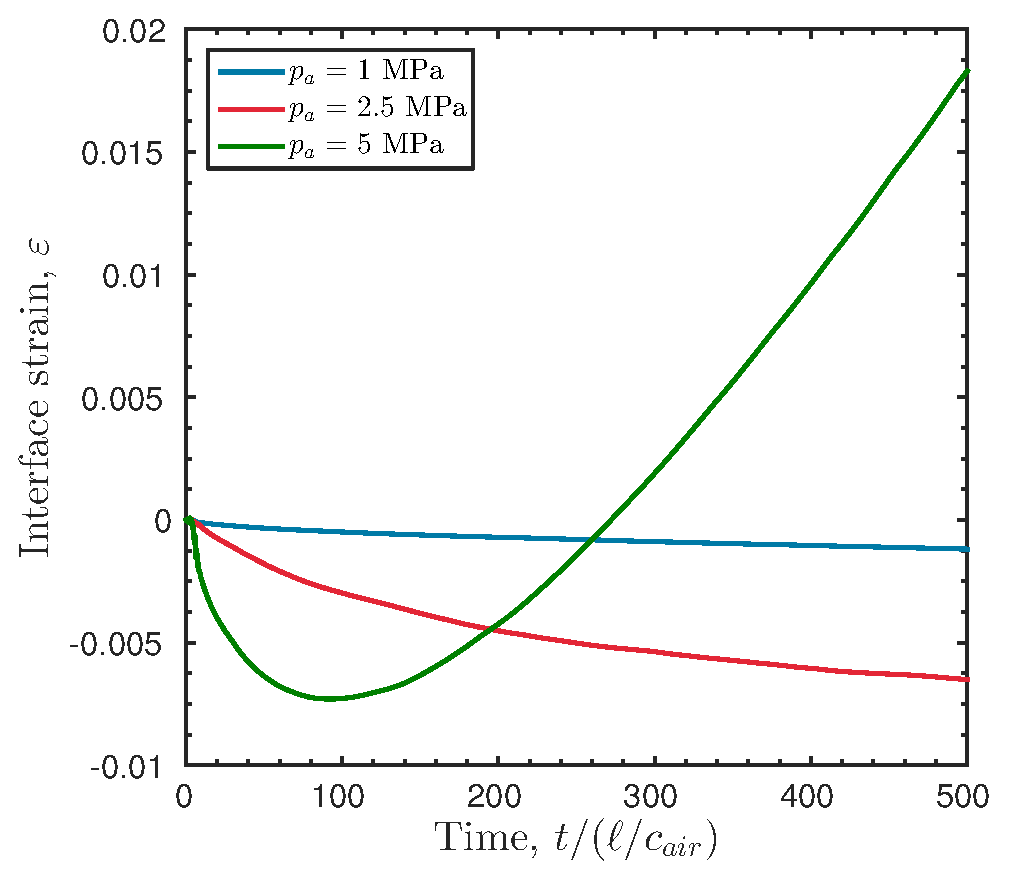
\includegraphics[width=\textwidth]{./figs/lung_figs/rmawave_1_A10,25,50_a03_strain_08-Mar-2017}
    \includegraphics[width=\textwidth]{./figs/lung_figs/rmawave_1_A10,25,50_a03_strain_15-Jun-2017_dim}
    \caption{\label{fig:strain_multi-pa_a03} $a_0 = 0.03\ell$}
  \end{subfigure}
  ~ 
  \begin{subfigure}[b]{0.49\textwidth}
    % 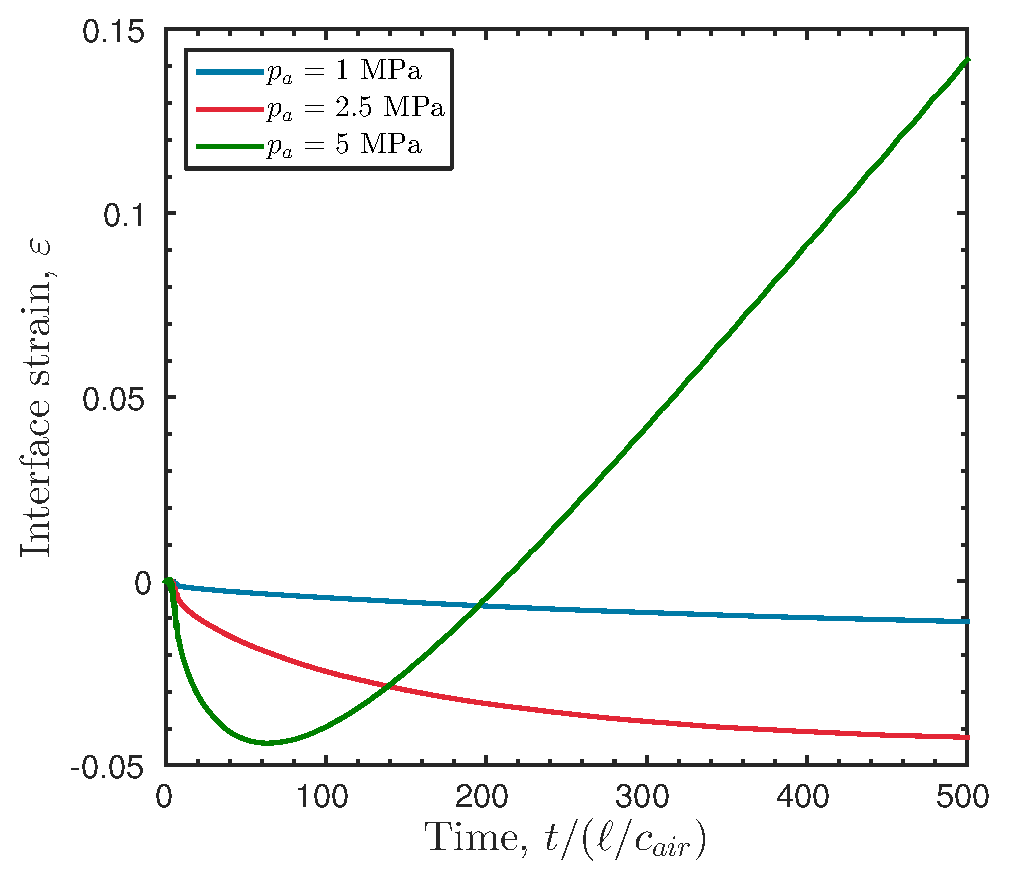
\includegraphics[width=\textwidth]{./figs/lung_figs/rmawave_1_A10,25,50_a10_strain_08-Mar-2017}
    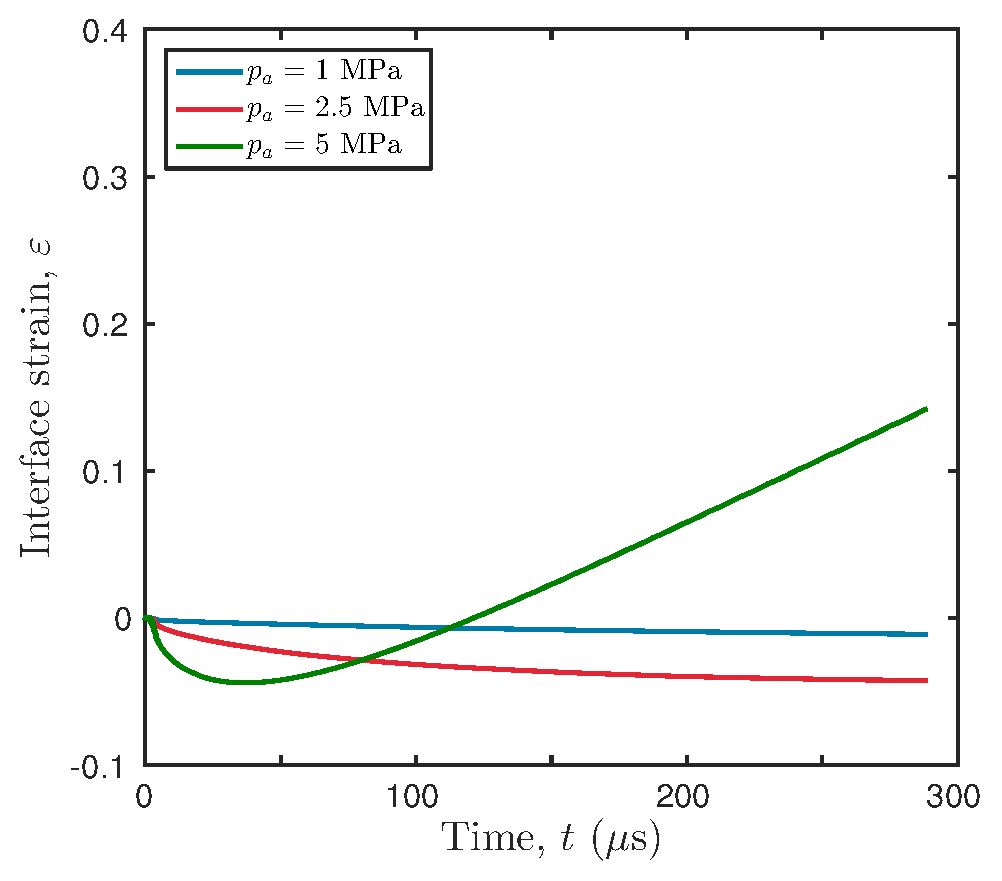
\includegraphics[width=\textwidth]{./figs/lung_figs/rmawave_1_A10,25,50_a10_strain_15-Jun-2017_dim}
    \caption{\label{fig:strain_multi-pa_a10} $a_0 = 0.10\ell$}
  \end{subfigure}
  ~ 
  \begin{subfigure}[b]{0.49\textwidth}
    % 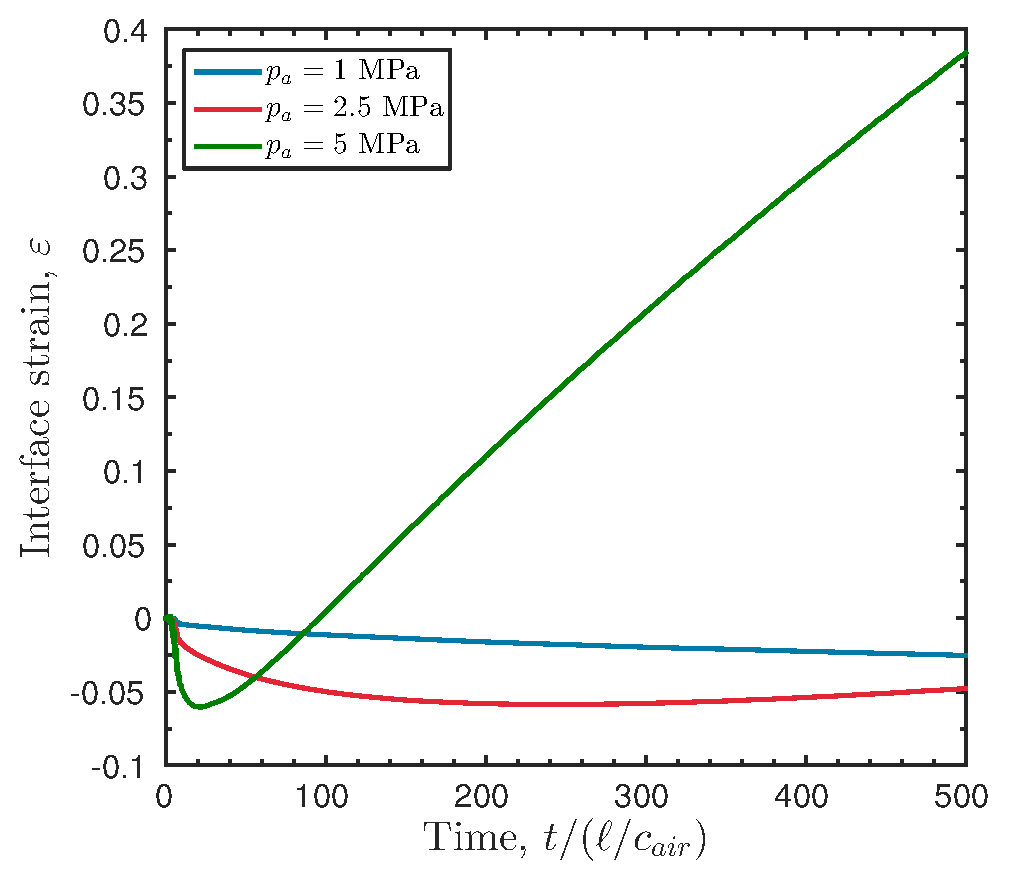
\includegraphics[width=\textwidth]{./figs/lung_figs/rmawave_1_A10,25,50_a30_strain_08-Mar-2017}
    \includegraphics[width=\textwidth]{./figs/lung_figs/rmawave_1_A10,25,50_a30_strain_15-Jun-2017_dim}
    \caption{\label{fig:strain_multi-pa_a30} $a_0 = 0.30\ell$}
  \end{subfigure}
  % 
  \caption[Interfacial strain dependence on pressure amplitude
  ($p_a=1.0, 2.5, 5.0$ MPa)]%
  {Interfacial strain dependence on pressure amplitude
    ($p_a=1.0, 2.5, 5.0$ MPa). Each plot shows $\varepsilon$ for a
    different initial condition: $a_0=0.03\ell$
    \subref{fig:strain_multi-pa_a03}, $0.10\ell$
    \subref{fig:strain_multi-pa_a10}, and $0.30\ell$
    \subref{fig:strain_multi-pa_a30}.}
  \label{fig:pa_dependence_strain}
\end{figure}
% 
\begin{figure}
  \centering
  \begin{subfigure}[b]{0.49\textwidth}
    % 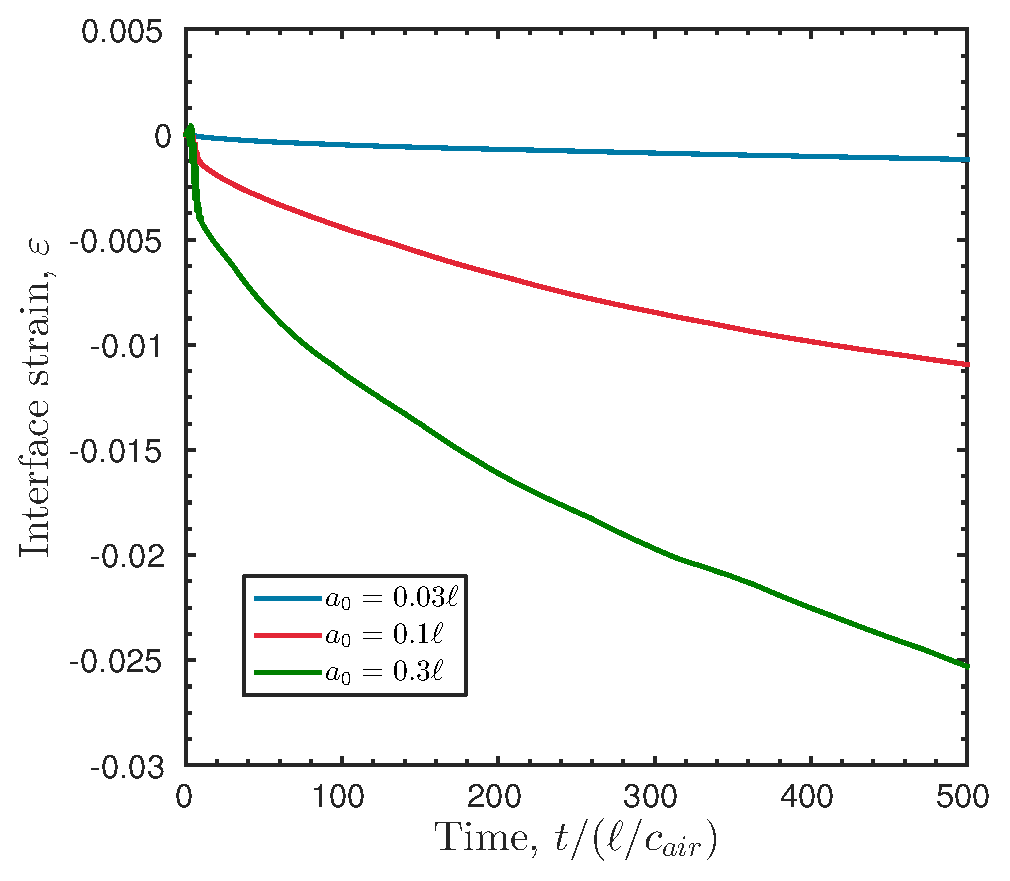
\includegraphics[width=\textwidth]{./figs/lung_figs/rmawave_1_A10_a03,10,30_strain_08-Mar-2017}
    \includegraphics[width=\textwidth]{./figs/lung_figs/rmawave_1_A10_a03,10,30_strain_15-Jun-2017_dim}
    \caption{\label{fig:strain_multi-a0-A10} $p_a = 1.0$ MPa}
  \end{subfigure}
  ~ 
  \begin{subfigure}[b]{0.49\textwidth}
    \includegraphics[width=\textwidth]{./figs/lung_figs/rmawave_1_A25_a03,10,30_strain_15-Jun-2017_dim}
    \caption{\label{fig:strain_multi-a0-A25} $p_a = 2.5$ MPa}
  \end{subfigure}
  ~
  \begin{subfigure}[b]{0.49\textwidth}
    % \includegraphics[width=\textwidth]{./figs/lung_figs/rmawave_1_A50_a03,10,30_strain_08-Mar-2017}
    \includegraphics[width=\textwidth]{./figs/lung_figs/rmawave_1_A50_a03,10,30_strain_15-Jun-2017_dim}
    \caption{\label{fig:strain_multi-a0-A50} $p_a = 5.0$ MPa}
  \end{subfigure}
  % 
  \caption[Interfacial strain dependence on initial perturbation
  amplitude ($a_0=0.03\ell,~0.10\ell,~0.30\ell$)]%
  {Interfacial strain dependence on initial perturbation amplitude
    ($a_0=0.03\ell,~0.10\ell,~0.30\ell$). Each plot shows $\varepsilon$
    for a different pulse amplitude: $p_a = 1.0 $ MPa
    \subref{fig:strain_multi-a0-A10}, $2.5$ MPa
    \subref{fig:strain_multi-a0-A25}, and $5.0$ MPa
    \subref{fig:strain_multi-a0-A50}.}
  \label{fig:a0_dependence_strain}
\end{figure}
% 
% 
\subsection{Viscous stress}
In further consideration of possible alveolar damage mechanisms, we
compute the inferred viscous shear stress field, based on the motion
of the inviscid flow, and the extract the maximum along the
interface. To illustrate the viscous stress around the interface,
color contours of the viscous stress fields are provided for the
$p_a = 5.0$ MPa wave in Figure \ref{fig:tauxy_snapshots} at
$t=2.9~\mu$s, approximately when the acoustic pulse and viscous stress
are at their maximum amplitudes. Subfigures
\subref{fig:tauxy_snapshot_A50_a03},
\subref{fig:tauxy_snapshot_A50_a10}, and
\subref{fig:tauxy_snapshot_A50_a30} again correspond to initial
perturbation amplitudes of $a_0 = 0.03\ell, 0.10\ell,$ and $0.30\ell$,
respectively. Black lines indicate isocontours of the volume fraction
of water $\alpha = 0.5$. Since the viscous shear stress is governed by
the velocity gradients in the fluid, which scale linearly with the
acoustic pressure gradients (See Equation
\ref{eq:acoustic_relations}), it is unsurprising that the greatest
viscous shear stress amplitudes occur during the wave-interface
interaction, and in particular close to the time when the maximum
pressure amplitude encounters the interface. The maximum viscous
stress is observed to occur in the lighter region of the interface, in
which the fluid is mostly air and the velocity gradients are
greatest. At this point in time, the fluid around the interface has
had little time to move as a result of the wave and consequently the
interface remains largely undeformed.

We extract the maximum viscous stress amplitudes from field
$\abs{\tau_{xy}}_{max}$, which were found to lie consistently along
the interface for all cases. To illustrate the dependence of
$\abs{\tau_{xy}}_{max}$ on the pulse amplitude $p_a$ and initial
perturbation amplitude $a_0$, Figure \ref{fig:pa_dependence_stress}
shows $\abs{\tau_{xy}}_{max}$ histories for variable $p_a = 1.0$
(blue), $2.5$ (red), and $5$ (green) MPa and constant initial
perturbation amplitude $a_0=0.03\ell$
\subref{fig:stress_multi-pa_a03}, $0.10\ell$
\subref{fig:stress_multi-pa_a10}, and $0.30\ell$
\subref{fig:stress_multi-pa_a30}, and Figure
\ref{fig:a0_dependence_stress} shows this data re-plotted for variable
$a_0 = 0.03\ell$ (blue), $0.10\ell$ (red), and $0.30\ell$ (green) and
constant wave amplitudes $p_a=1.0$ \subref{fig:stress_multi-a0-A10},
$2.5$ \subref{fig:stress_multi-a0-A25}, and $5.0$
\subref{fig:stress_multi-a0-A50} MPa. We highlight the fact that,
because we are intentionally only interested in the maximum
interfacial stress amplitude, the location along the interface at
which $\abs{\tau_{xy}}_{max}$ occurs changes in time, which is not
captured in the figures. For all waves and initial perturbation
conditions, $\abs{\tau_{xy}}_{max}$ oscillates with the wave during
the wave interaction, around a mean value which appears to rise and
fall with the acoustic intensity. We note that there is a component of
these oscillations that coincide with the fluctuations in the \ac{US}
pulse. These fluctuations occurs at approximately twice the pulse
frequency because we are considering the absolute value of the viscous
stress, which we expect to scale with the magnitude of the velocity
gradients and therefore the pulse amplitude (see the acoustic
relationships described in Chapter \ref{ch:usbe_lung}).

It is clear from both Figure \ref{fig:pa_dependence_stress} and
\ref{fig:a0_dependence_stress} that, on average, increasing the wave
amplitude increases the viscous stress amplitude at the interface as
expected (neglecting chronologically local oscillations). Regarding
the dependence of $\abs{\tau_{xy}}_{max}$ on $a_0$, we make two
observations. First, as $a_0$ increases, the chronologically local
mean value of $\abs{\tau_{xy}}_{max}$ also increases, though this is
slightly less obvious from the figures due to the varying degree of
oscillation between the curves. Second, based on differences between
Figures
\ref{fig:pa_dependence_stress}\subref{fig:stress_multi-a0-A10},
\subref{fig:stress_multi-a0-A25}, and
\subref{fig:stress_multi-a0-A50}, as $a_0$ increases, the oscillation
behavior changes. The overall magnitude of the osccillations in
$\abs{\tau_{xy}}_{max}$, relative to the chronologically local mean,
decreases. This is because as $a_0$ increases, a greater portion of
the reflected wave propagates in the transverse direction. These
transverse waves introduce additional oscillations in the shear stress
field, which are small when compared to those generated directly by
the incoming wave. These oscillations are identified according to
their timing and are most clearly explained with an example. Consider
$\abs{\tau_{xy}}_{max}$ for the $p_a=5$ MPa, $a_0=0.3\ell$ case, as
shown in Figure
\ref{fig:a0_dependence_strain}\subref{fig:strain_multi-a0-A50}. The
larger stress peaks occur approximately regularly during the wave
interaction every $0.3~\mu$s, and correspond to the interactions of
the peaks and troughs of the wave with the interface, as shown in
Figure \ref{fig:p0_ultrasound}. Shortly after each of these larger
peaks there is a slight drop in the peak stress. The time separating
the peak and drop is approximately $\ell/c\approx0.12~\mu$s,
indicating these fluctuations are a consequence of the transversely
reflected wave, which has the opposite sign of the incoming wave. We
note that axial reflections are small and do not return to the
interface until after the passage of the initial wave. After the
passage of the wave, the maximum shear stress drops to nearly zero in
all cases.

In consideration of \ac{DUS}-induced alveolar hemorrhage, we note that
for the parameters considered here the maximum viscous stress
amplitudes observed at the interface occur during the interaction with
the wave and ranged from $2$ to $61$ Pa. Even
the greatest observed stress is two orders of magnitude smaller the
$8$ kPa minimal stress failure threshold observed by \cite{West1991}
for disruption of alveolar epithelium. These stresses occur during
the wave-interface interaction, and quickly fall off thereafter, in
much less time than a typical period between pulses ($\sim 1$
ms). This suggests that viscous stresses are not likely to quickly
accumulate between pulses. A possible, exception to this could occur
if the velocity field were to change significantly, perhaps as a
result of accumulated vorticity from subsequent \ac{US} pulses. The
computational cost of testing this possibility numerically is not feasible under
the current framework, and as such is beyond the scope of this work.
% 
% 
\begin{figure}
  \captionsetup[subfigure]{labelformat=empty}
  \centering
  \begin{subfigure}[b]{0.3\textwidth}
    \begin{tikzpicture}%
      \node[anchor=south west,inner sep=0] (image) at (0,0) {
        \includegraphics[width=\textwidth]{./figs/lung_figs/rmawave_1_A50_a03_t005_tauxy_snapshots_dim_printable}
      };%
      \begin{scope}[x={(image.south east)},y={(image.north west)}]%
        \node[font=\small,right] at (0.2,0.9) {$\tau_{xy}$ (Pa)};%
        \node[font=\small,right] at (0.2,0.25) {$t = 2.9~\mu$s };%
      \end{scope}%  
    \end{tikzpicture}%
    \caption{\label{fig:tauxy_snapshot_A50_a03} $a_0 = 0.03\ell$}
  \end{subfigure}
  ~ 
  \begin{subfigure}[b]{0.3\textwidth}
    \begin{tikzpicture}%
      \node[anchor=south west,inner sep=0] (image) at (0,0) {
        \includegraphics[width=\textwidth]{./figs/lung_figs/rmawave_1_A50_a10_t005_tauxy_snapshots_dim_printable}
      };%
      \begin{scope}[x={(image.south east)},y={(image.north west)}]%
        \node[font=\small,right] at (0.2,0.9) {$\tau_{xy}$ (Pa)};%
        \node[font=\small,right] at (0.2,0.25) {$t = 2.9~\mu$s };%
      \end{scope}%  
    \end{tikzpicture}%
    \caption{\label{fig:tauxy_snapshot_A50_a10} $a_0 = 0.10\ell$}
  \end{subfigure}
  ~ 
  \begin{subfigure}[b]{0.3\textwidth}
    \begin{tikzpicture}%
      \node[anchor=south west,inner sep=0] (image) at (0,0) {
        \includegraphics[width=\textwidth]{./figs/lung_figs/rmawave_1_A50_a30_t500_tauxy_snapshots_dim_printable}
      };%
      \begin{scope}[x={(image.south east)},y={(image.north west)}]%
        \node[font=\small,right] at (0.2,0.9) {$\tau_{xy}$ (Pa)};%
        \node[font=\small,right] at (0.2,0.25) {$t = 2.9~\mu$s };%
      \end{scope}%  
    \end{tikzpicture}%
    \caption{\label{fig:tauxy_snapshot_A50_a30} $a_0 = 0.30\ell$}
  \end{subfigure}
  \caption[Evolution of the viscous stress field for the $p_a=5.0$ MPa
  wave]{Evolution of the viscous stress field for the $p_a=5.0$ MPa
    wave. Contour plots of the Newtonian viscous stress $\tau_{xy}$ in
    Pascals are shown for each initial perturbation amplitude, at
    $t=5$, near the point when the maximum stress occurs. In Figures
    \subref{fig:tauxy_snapshot_A50_a03},
    \subref{fig:tauxy_snapshot_A50_a10}, and
    \subref{fig:tauxy_snapshot_A50_a30} $a_0=0.03\ell,\, 0.10\ell,$ and
    $0.30\ell$ respectively.  }
  \label{fig:tauxy_snapshots}
  % 
\end{figure}

% \begin{comment}
%   \begin{figure}
%     \centering
%     \begin{subfigure}[b]{0.32\textwidth}
%       \begin{tikzpicture}%
%         \node[anchor=south west,inner sep=0] (image) at (0,0) {
%         \includegraphics[width=\textwidth]{./figs/lung_figs/rmawave_1_A50_a03_t005_tauxy_snapshots}
%       };%
%         \begin{scope}[x={(image.south east)},y={(image.north
%           west)}]%
%           \node[font=\small,right] at (0.75,0.05) {$\tau_{xy}$
%           (Pa)};%
%         \end{scope}%
%       \end{tikzpicture}%
%       \caption{\label{fig:tauxy_snapshot_A50_a03} $a_0 = 0.03\ell$}
%     \end{subfigure}
%     ~
%     \begin{subfigure}[b]{0.32\textwidth}
%       \begin{tikzpicture}%
%         \node[anchor=south west,inner sep=0] (image) at (0,0) {
%         \includegraphics[width=\textwidth]{./figs/lung_figs/rmawave_1_A50_a10_t005_tauxy_snapshots}
%       };%
%         \begin{scope}[x={(image.south east)},y={(image.north
%           west)}]%
%           \node[font=\small,right] at (0.75,0.05) {$\tau_{xy}$
%           (Pa)};%
%         \end{scope}%
%       \end{tikzpicture}%
%       \caption{\label{fig:tauxy_snapshot_A50_a10} $a_0 = 0.10\ell$}
%     \end{subfigure}
%     ~
%     \begin{subfigure}[b]{0.32\textwidth}
%       \begin{tikzpicture}%
%         \node[anchor=south west,inner sep=0] (image) at (0,0) {
%         \includegraphics[width=\textwidth]{./figs/lung_figs/rmawave_1_A50_a30_t500_tauxy_snapshots}
%       };%
%         \begin{scope}[x={(image.south east)},y={(image.north
%           west)}]%
%           \node[font=\small,right] at (0.75,0.05) {$\tau_{xy}$
%           (Pa)};%
%         \end{scope}%
%       \end{tikzpicture}%
%       \caption{\label{fig:tauxy_snapshot_A50_a30} $a_0 = 0.30\ell$}
%     \end{subfigure}
%     %     
%     \caption{Contour plots of the Newtonian viscous stress
%     $\tau_{xy}$ in Pascals are shown for each initial perturbation
%     amplitude for the $p_a=5.0$ MPa pulse at $t=5$, near the point
%     when the maximum stress occurs. In Figures
%     \subref{fig:tauxy_snapshot_A50_a03},
%     \subref{fig:tauxy_snapshot_A50_a10}, and
%     \subref{fig:tauxy_snapshot_A50_a30} $a_0=0.03\ell,\, 0.10\ell,$
%     and $0.30\ell$ respectively.  }
%     \label{fig:tauxy_snapshots}
%   \end{figure}
% \end{comment}
% 
\begin{figure}
  \centering
  \begin{subfigure}[b]{0.49\textwidth}
    % \includegraphics[width=\textwidth]{./figs/lung_figs/rmawave_1_A10,25,50_a3_tauxy_27-Feb-2017}
    \includegraphics[width=\textwidth]{./figs/lung_figs/rmawave_1_A10,25,50_a03_tauxy_07-Mar-2017_dim}
    \caption{\label{fig:stress_multi-pa_a03} $a_0 = 0.03\ell$}
  \end{subfigure}
  ~ 
  \begin{subfigure}[b]{0.49\textwidth}
    % \includegraphics[width=\textwidth]{./figs/lung_figs/rmawave_1_A10,25,50_a10_tauxy_27-Feb-2017}
    \includegraphics[width=\textwidth]{./figs/lung_figs/rmawave_1_A10,25,50_a10_tauxy_07-Mar-2017_dim}
    \caption{\label{fig:stress_multi-pa_a10} $a_0 = 0.10\ell$}
  \end{subfigure}
  ~ 
  \begin{subfigure}[b]{0.49\textwidth}
    % \includegraphics[width=\textwidth]{./figs/lung_figs/rmawave_1_A10,25,50_a30_tauxy_27-Feb-2017}
    \includegraphics[width=\textwidth]{./figs/lung_figs/rmawave_1_A10,25,50_a30_tauxy_07-Mar-2017_dim}
    \caption{\label{fig:stress_multi-pa_a30} $a_0 = 0.30\ell$}
  \end{subfigure}
  % 
  \caption[Interfacial viscous stress dependence on pressure
  amplitude ($p_a=1.0, 2.5, 5.0$ MPa)]{Interfacial viscous stress
    dependence on on pressure amplitude ($p_a=1.0, 2.5, 5.0$ MPa). Each
    plot shows $\left|\tau_{xy}\right|_{max}$ for a different initial
    condition: $a_0=0.03\ell$ \subref{fig:stress_multi-pa_a03},
    $0.10\ell$ \subref{fig:stress_multi-pa_a10}, and $0.30\ell$
    \subref{fig:stress_multi-pa_a30}.}
  \label{fig:pa_dependence_stress}
\end{figure}
% 
\begin{figure}
  \centering
  \begin{subfigure}[b]{0.49\textwidth}
    \includegraphics[width=\textwidth]{./figs/lung_figs/rmawave_1_A10_a3,10,30_tauxy_27-Feb-2017_dim}
    \caption{\label{fig:stress_multi-a0-A10} $p_a = 1.0$ MPa}
  \end{subfigure}
  ~
  \begin{subfigure}[b]{0.49\textwidth}
    \includegraphics[width=\textwidth]{./figs/lung_figs/rmawave_1_A25_a3,10,30_tauxy_27-Feb-2017_dim}
    \caption{\label{fig:stress_multi-a0-A25} $p_a = 2.5$ MPa}
  \end{subfigure}
  ~ 
  \begin{subfigure}[b]{0.49\textwidth}
    \includegraphics[width=\textwidth]{./figs/lung_figs/rmawave_1_A50_a3,10,30_tauxy_27-Feb-2017_dim}
    \caption{\label{fig:stress_multi-a0-A50} $p_a = 5.0$ MPa}
  \end{subfigure}
  % 
  \caption[Interfacial viscous stress dependence on initial
  perturbation amplitude amplitude
  ($a_0=0.03\ell, 0.10\ell, 0.30\ell$)]{Interfacial viscous stress
    dependence on initial perturbation amplitude amplitude
    ($a_0=0.03\ell, 0.10\ell, 0.30\ell$). Each plot shows
    $\left|\tau_{xy}\right|_{max}$ for a different pulse amplitude:
    $p_a = 1.0$\subref{fig:stress_multi-a0-A10},
    $2.5$\subref{fig:stress_multi-a0-A25}, and
    $5.0$\subref{fig:stress_multi-a0-A50} MPa.}
  \label{fig:a0_dependence_stress}
\end{figure}
% 
% 
% 
% 
% 
% 
\subsection{Ultrasound-induced vorticity dynamics and interface growth}
\label{subsec:vorticity_experiments}
Having examined the stresses and strains associated with liquid-gas
interfaces driven by \ac{US} pulse waves, within the regime relevant
to clinical \ac{DUS}, we now hypothesize that the observed deformation
is driven by baroclinic vorticity deposited at the liquid-gas
interface by the \ac{US} pulse. As there is still a highly nonlinear
density gradient across the interface, misaligned with strong
ultrasonic pressure gradients, the potential for meaningful baroclinic
vorticity deposition, and consequently persistent of the system,
exists. As we demonstrated that this was possible for a trapezoidal
acoustic wave in Chapter \ref{ch:usbe_lung}, we consider a second set
of experiments, designed to test if this holds true for the ultrasound
pulse. We will compare the interface and vorticity dynamics of an
ultrasound driven pulse, with those of the trapezoidal pulse of the
Chapter \ref{ch:usbe_lung}. The $1.0$ to $5.0$ MPa pulses used earlier
in this chapter drive the system too slowly for the interface growth
to reach its late-time behavior within a computationally feasible
period. Additionally, we aim to compare to our previous results and as
such we choose our acoustic pulse parameters and initial interface
perturbation amplitude to match that of our baseline trapezoidal wave
case Chapter \ref{ch:usbe_lung}: $a_0=0.03\ell$; $p_a = 10$ MPa;
$L=45\ell$. To further facilitate comparison of this experiment to
those of the previous chapter, all results presented here will be
non-dimensionalized by $\ell$ and $c_{water}$ unless otherwise
indicated.

To illustrate the vorticity during and after the passage of the wave,
Figure \ref{fig:Vorticity_circ_us}\subref{fig:us_vorticity_snapshot}
shows vorticity contours for the $p_a = 10$ MPa pulse wave case, at
$t/(\ell/c) = 4.75$ and $90$ (or $t = 0.6 $ and $12~\mu$s). It can be
clearly seen that vorticity is deposited along the interface by the
ultrasound wave, and remains after its passing. In consideration of a
quantitative, cumulative measure of vorticity deposited by the
ultrasound wave we integrate the vorticity at over the right-half
domain for each point in time to obtain the circulation,
$\Gamma(t)$. Figure
\ref{fig:Vorticity_circ_us}\subref{fig:us10_circulation_history} plots
the right-half domain circulation history during the wave interaction
and shortly thereafter. The end of the interaction between the
incident wave and the interface is indicated as a black, dashed
vertical line $t/(\ell/c) = 47.5$. It can be seen that the wave
deposits circulation, which remains approximately constant after its
passage. The circulation left at the end of the wave is approximately
$3 \times 10^{-4}$, which is roughly $1/5$ that left by the $p_a = 10$
MPa trapezoidal wave in Chapter \ref{ch:usbe_lung}. We note that
unlike the trapezoidal wave, which consists entirely of positive
pressure, the \ac{US} pulse consists of cyclic positive and negative
pressure, such that each subsequent cycle is expected to deposit
vorticity of sign opposite that of the previous cycle, since a phase
inversion of the interface perturbation was not observed during the
wave-interface interaction. Hence it is perhaps unsurprising that less
circulation is deposited by the ultrasound pulse than by the
trapezoidal wave of equivalent maximum amplitude. As in the previous
chapter, the circulation in the left-half domain is equal and opposite,
such that the total circulation is zero. Similar circulation histories
for the $p_a = 1.0, 2.5,$ and $5.0$ MPa waves, used in the earlier
stress and strain calculations, are provided in Appendix
\ref{sec:us_pulse_circulation}, and reveal that similar to the
$p_a = 10$ MPa case, circulation remains after the passage of the
wave. Appendix \ref{sec:us_pulse_circulation} also explores the
dependence of that circulation on $a_0$ and $p_a$ for the case of the
ultrasound pulse.%
\begin{figure}
  \centering
  \vfill
  \begin{subfigure}[t]{0.6\textwidth}
    \centering
    \begin{tikzpicture}
      \node[anchor=south west,inner sep=0] (image) at (0,0) {%
        \includegraphics[height=0.49\textwidth]{./figs/lung_figs/vorticity_t1_rmawave_1_10000000,0_0,03_45,0_0,0_1,0_1,0_1000_100_01-Aug-2017}
        \includegraphics[height=0.49\textwidth]{./figs/lung_figs/vorticity_t20_rmawave_1_10000000,0_0,03_45,0_0,0_1,0_1,0_1000_100_nocb}
      };%
      \begin{scope}[x={(image.south east)},y={(image.north west)}]%
        \node[font=\small,align=left,right] at (0.1,0.9){{$t=4.75$}};%
        \node[font=\small,align=left,right] at (0.4,0.9){{$(a)$}};%
        \node[font=\small,align=left,right] at (0.6,0.9){{$t=95$}};%
      \end{scope}%
    \end{tikzpicture}
    \phantomcaption%{Vorticity Contours}
    \label{fig:us_vorticity_snapshot}
  \end{subfigure}
  \hfill
  ~
  \begin{subfigure}[t]{0.35\textwidth}
    \begin{tikzpicture}
      \node[anchor=south west,inner sep=0] (image) at (0,0) {%
        \includegraphics[width=\textwidth]{./slides/figs/trapz_us_circ_comparison_A10_waveend_t0_t60_asa_01-Aug-2017}
      };%
      \begin{scope}[x={(image.south east)},y={(image.north west)}]%
        \node[font=\small,align=left,right] at
        (0.85,0.85){{(b)}};%
      \end{scope}%
    \end{tikzpicture}
    \phantomcaption%{Circulation, $\Gamma = \int_{A_R} \omega dA$}
    \label{fig:us10_circulation_history}
  \end{subfigure}
  \caption[Vorticity and circulation histories for the $p_a=10$ MPa
  ultrasound pulse.]{Vorticity and circulation histories for the
    $p_a=10$ MPa ultrasound pulse. \subref{fig:us_vorticity_snapshot}
    Vorticity contours during the wave interaction, at
    $t/(\ell/c)=4.75$ and after its passage at
    $t/(\ell/c)=90$. \subref{fig:us10_circulation_history} The
    dimensionless circulation history. The passage of the wave at
    $t/(\ell/c)=47.5$ is indicated as a black, dashed vertical line.}
  \label{fig:Vorticity_circ_us}
\end{figure}%

To compare the late time growth of the perturbation amplitude driven
by the ultrasound wave, with that driven by the trapezoidal wave,
Figure \ref{fig:us10_interface_growth} displays the perturbation
amplitude history $a(t)/a_0$ on a log-log scale. For
$t/(\ell/c)\leq 4000$ we calculate the interface perturbation
amplitude growth exponent $t^n$, as was done in Chapter
\ref{ch:usbe_lung} and find that $n = 0.57$. This result is consistent
with the $t^{3/5}$ power-law growth obtained for a trapezoidal wave in
Chapter \ref{ch:usbe_lung}.
\begin{figure}
  \captionsetup[subfigure]{labelformat=empty}
  \centering
  \centering
  \begin{tikzpicture}
    \node[anchor=south west,inner sep=0] (image) at (0,0) {%
      \includegraphics[width=0.5\textwidth]{./slides/figs/trapz_us_amp_comparison_A10_waveend_asa_01-Aug-2017}
      % \includegraphics[width=\textwidth]{./figs/trapz_us_amp_comparison_A10_waveend}
    };%
    % \begin{scope}[x={(image.south east)},y={(image.north west)}]%
    %   \node[font=\scriptsize,align=left,right] at
    %   (0.2,0.9){{$t=1$}};%
    % \end{scope}%
  \end{tikzpicture}
  \caption[Interface perturbation amplitude history for the
  $p_a=10$ MPa ultrasound pulse.]{Interface perturbation amplitude
    history for the $p_a=10$ MPa ultrasound pulse. $a(t)/a_0$ is
    plotted vs time on a log-log scale. $t^{3/5}$ growth is
    indicated by the dashed black line.}
  \label{fig:us10_interface_growth}
\end{figure}%
% 
% In Chapter \ref{ch:usbe_lung} it was demonstrated that interface
% deformations that occurred following trapezoidal acoustic waves were
% indeed driven by baroclinic vorticity. And at the beginning of this
% chapter, we hypothesized that ultrasound waves may also be capable of
% generating baroclinic vorticity at alveolar interfaces within the
% lungs, and thus capable of inducing strains which may partially
% account for some of the lung hemorrhage observed as a result of
% \ac{DUS}. Unlike the trapezoidal waves of Chapter \ref{ch:usbe_lung},
% which had positive definite pressure profiles, the \ac{US} waves have
% cyclically positive and negative pressure profiles, which we
% intuitively expect to deposit vorticity of opposite sign on each
% subsequent cycle, and thus less total circulation after the passage of
% the wave.

After the passage of the \ac{US} pulse, there are no obvious
mechanisms, beside baroclinic vorticity, to drive the continued
deformation of the interface. As such, it is worth discussing what
precisely contributes to the circulation remaining after the passage
of the wave. Throughout the wave-interface interaction, the interface
itself deforms such that while \ac{US} pressure gradient is
continuously misaligned with portions of the interface density
gradient, though the degree of that misalignment changes in time along
the entire interface. While this deformation appears to be nominally
small (note the barely observable difference between frames 1 and 2
for each subfigure within Figures \ref{fig:rho_snapshots_A10},
\ref{fig:rho_snapshots_A25}, \ref{fig:rho_snapshots_A50}), it is
finite, calculable, and critical to the vorticity dynamics. Because
the pressure returns to ambient after the passage of the wave, it must
be true that the integral of the acoustic pressure gradient over all
time is zero, just as it was for the trapezoidal wave. Thus the only
way that baroclinic vorticity can remain after the passage of the wave
is through changes in the density gradient during the interaction. As the interface deforms
the direction these small changes in the direction and local magnitude
of the density gradient result in a net deposition of circulation that
remains to deform the interface after the passage of the wave. This
has particular relevance to ultrasound which relies on many subsequent
pulses, potentially resulting in the accumulation of vorticity over
time.
% 

\subsection{Limitations of the present work}
The model of an ultrasound-driven alveolus used in this work is
exactly that, a model. This work aims only to offer insight into the
physics and potential physical damage mechanisms of \ac{DUS}-induced
lung hemorrhage. Our approximation of the physical system is perhaps
not a particularly, naturally intuitive one. Moreover the vorticity
mechanisms that we suggest are driving the system are not intuitive
for a viscoelastic solid. The concept of vorticity, even in a
viscoelastic solid (e.g., soft tissue), can be thought of rather
simply at a fixed instant in terms of a velocity magnitude (not
direction) difference between opposite sides of a particle of
continuum, such that the instantaneous tendency of the particle is to
rotate. Our conceptual arguments for overcoming this arise out of our
understanding of this as a continuum of viscoelastic solids, which may
act as a solid or liquid depending on the physical regime of
interest. The model is based on highly fundamental laws of mechanics
(conservation of mass, momentum, energy) and neglected physical
effects are justified in the relevant regime based on dimensional
analysis. Additionally, the problem geometry and setup are chosen
based on the relevant application. While the author recognizes that
treatment of an alveolar septum as a perturbed water-air interface
intuitively seems a bit too simple, all of the dimensional and order
of magnitude arguments suggest that specifically for the timescales
considered here, the simulated dynamics are reasonable. Though there
are several limitations to this study that would not allow the
simulated physics to capture the physics of diagnostic
ultrasound-alveolar interactions over longer time spans. Here we
specifically consider limitations that arise from our constitutive
model of the lung tissue and the model problem geometry. Based on our
physical understanding, it is not unreasonable to speculate about how
each of these limitations is likely to effect the simulated physics.

In this study, we treat the alveolar septa and capillaries therein as
a liquid-gas interface, and within our physical model we neglect
certain physical features characteristic of soft tissue, including
viscoelasticity and the mechanical failure. Rather than repeat the
dimensional analysis arguments used to initially justify the model in
Chapters \ref{ch:Introduction} and \ref{ch:usbe_lung} we will consider
how each of these could affect the physical system. Viscosity and
elasticity both have potential importance at late times. In the
context of the present work, viscosity may act to serve as a mechanism
to dissipate vorticity, thus reducing strain on the
interface. However, the characteristic timescale over which we expect
the vorticity to dissipate over a relevant area $\sim\ell^2/\nu_{air}$
is multiple milliseconds, and is thus unlikely to greatly effect the
dynamics over the considered period. Elasticity is likely to provide a
restoring force to resist the deformation of the interface, however
this is likely to be small relative to the fluid inertia, which we
show quantitatively in Appendix
\ref{sec:elasticity_appendix}. Additionally, this model is no longer
valid after the alveolar septum fails, which may occur in some of our
simulations based on the considered failure criteria. As the strains
observed are large, before the elastic force is likely to overcome the
fluid inertia, the elastic restorative force may not be particularly
useful at mitigating vorticity-induced strain. Many of these specific
limitations are in part a result of limitations of the existing body
of knowledge concerning the mechanical properties and failure behavior
of alveolar tissue under stresses and strains, which is poorly
characterized within the timescales and physical regimes relevant
here. We highlight the fact that the available stress and strain
failure criteria available for alveoli are based on much slower
processes than occur during \ac{DUS}, making for an imperfect
comparison at best. Additionally, the stress $8$ kPa stress failure
criterion of \cite{West1991} is for wall stress, which is not the same
as shear, but was the best available metric at the time of this
writing.

In consideration of the limitations of our model geometry, we will
start from the fact that this work aims only to study interactions
between a single ultrasound pulse and a single alveolus. As such we
consider the effect of a treating the alveolar septum as a slightly
perturbed sinusoidal interface between fluids. In comparison to the
histological slide of alveoli shown in Figure
\ref{fig:alveolar_histology}, the geometry considered here is smoother
and flatter than true alveolar boundaries. As such, there is the
potential for greater shear stress concentrations and baroclinic
vorticity generation with subsequent strain in the real physical
system. Additionally, the 2D representation of the problem as a single
alveolus neglects any physical support the system may receive from its
surroundings. And while it has been suggested that pulmonary
capillaries are largely unsupported by surrounding tissues
\citep{West1991}, without quantification of that support, it is
possible that it would help to reduce vorticity-driven motion of the
interface, particularly at the edges. However, the deformation and
strain observed here is largely driven by vorticity local to the
interface perturbation, such that it would likely not be greatly
effected by such support. Lastly, we acknowledge that this model
cannot capture 3D fluid effects (e.g., turbulence, vortex-stretching,
etc...) that are expected to be negligible over the timescales
considered based on the Reynolds number and order of magnitude
analysis of the individual terms of the vorticity equation (see
Appendix \ref{sec:oom_analysis}).

\section{Summary, conclusions, and future work}
\label{sec:usbe_lung_bio_conclusions}
In summary, \ac{US} pulse waves were simulated propagating from water
into sinusoidally perturbed water-air interfaces to model a single
\ac{US}-pulse impinging upon an alveolus from surrounding soft
tissue. We assume a typical adult mean alveolar diameter of
$\ell=200~\mu$m \citep{Ochs2004} as a characteristic length scale,
such that the maximum simulation time was approximately $288~\mu$s. To
estimate viscous stresses and interfacial linear strains relevant to
\ac{DUS}-induced alveolar hemorrhage, 1.5 MHz ultrasound pulse waves
with amplitudes of $p_a=1.0, 2.5,$ and $5.0$ MPa were used. Initial
interface perturbation amplitudes of $a_0= 0.03\ell, 0.10\ell,$ and
$0.30\ell$ were considered. For each case, the wave-interface
interaction generated vorticity along the interface and resulted in
long-term deformation of the interface, which continued well after the
passage of the wave. Relevant calculations of the density fields,
inferred viscous stress fields, and linear interfacial strain within
the simulated period are reported. The computed peak interface strain
amplitudes $\abs{\varepsilon}$ ranged from $0.01$ to $0.38$. During
the computed period, only for the $5.0$ MPa wave did strains exceed the
$\abs{\varepsilon}=0.08$ damage threshold, reported by
\cite{Belete2010}. The peak passive viscous stress estimates at the
interface were on the order of tens of Pascals, which is far below the
$8$ kPa stress failure criterion reported by \cite{West1991}. A second
experiment was performed to determine that baroclinic vorticity is the
driver of the observed deformation. For this experiment, a $p_a = 10$
MPa pulse was propagated toward a perturbed water-air interface of
amplitude $a_0 = 0.03\ell$ and the vorticity and interface dynamics
were compared to those of the trapezoidal waves in Chapter
\ref{ch:usbe_lung}. It was found that ultrasound pulses deposited
circulation of similar distribution and order of magnitude to those
previously observed for the trapezoidal waves. The perturbation was found
to grow approximately as $t^{3/5}$, as was expected for baroclinic
vorticity-driven growth, based on our previous work.

This work is a first step toward investigating the possibility of
baroclinic vorticity-induced strain as potential mechanism for
ultrasound-induced alveolar hemorrhage. This work is novel in its
modeling using the nonlinear equations of fluid motion to study the
dynamics of an alveolus interacting with a single \ac{DUS}
pulse. Furthermore, this work is unique in its comparison of alveolar
stress and strain estimates with previously determined failure
criteria. While the calculated stresses and strains observed based on
the interaction between an air water interface and a single ultrasound
pulse may be representative of some of the physics associated with
\ac{DUS}-alveolar interactions, we cannot confidently say that
baroclinic vorticity is the likely cause of \ac{DUS}-induced
hemorrhage in the lung. As true \ac{DUS} typically involves many
subsequent pulses, further investigations will need to account for
this. However, based on the work reported here, we draw the following
conclusions:
\begin{enumerate}
\item \textbf{Newtonian, viscous stress alone is unlikely to be
    sufficient to cause \ac{DUS}-induced hemorrhage of the alveolar
    wall}. While many approximations and simplifications were made
  throughout the course of this work, the work presented estimates
  \textit{worst case} viscous shear stresses. Here, the velocity
  gradients are higher than would be expected in the true physical
  system because neglected viscous and elastic effects would resist
  interfacial motion in the true physical system. In spite of this,
  the calculated shear stresses are multiple orders of magnitude less
  than expected alveolar stress failure thresholds.
\item \textbf{\ac{DUS} pulses within clinically relevant regimes have
    the potential to deposit baroclinic vorticity within gas-liquid
    interfaces in the lungs, which is capable of driving deformation.}
  This work clearly demonstrates that diagnostically relevant
  ultrasound pulses are capable of creating lasting baroclinic
  vorticity at liquid-gas interfaces which are dynamically similar to
  alveolar tissue-gas interfaces. For the $10$ MPa case, the interface
  perturbation exhibits $\sim t^{3/5}$ power-law growth at late times,
  as was previously shown to occur for interfaces driven by
  trapezoidal acoustic waves. For weaker waves, running the
  simulations to sufficiently late time to observe this behavior was
  too computationally costly to be done. This indicates that
  ultrasonically driven vorticity is a viable mechanism for driving
  the observed growth. The observed interfacial strains created by
  pulses as weak $p_a = 5.0$ MPa were more than sufficient to cause
  damage based on previously observed alveolar failure
  criteria. Furthermore, based on dimensional arguments, dissipation
  of the observed vorticity is expected to occur over multiple
  milliseconds, which is greater than the typical time between
  subsequent \ac{DUS} pulses. Hence \ac{US} may be capable of
  accumulating vorticity in the lungs over several subsequent pulses
  and thus driving greater deformation. This will depend on the
  morphology of the interface during the arrival of each pulse, which
  is likely to vary widely depending on the initial conditions and
  ultrasound parameters, as the minimum strain cases showed
  practically no deformation over a third of a typical pulse interval,
  and the large strain cases are likely to cause alveolar failure
  before subsequent pulses arrive. 
\end{enumerate}



%%%%%%%%%%%%%%%%%%%%%%%%%%%%%%% 
% \section{conclusions and future work}


% \begin{comment}
%   Among the tissue layers%   The anatomical structure of the lungs has been studied extensively
%   and is of particular interest to the present work. The alveoli can
%   be thought of as a network of openly connected, air-filled saccules
%   with distinctly irregular surfaces. And while alveoli are
%   irregularly shaped and do not have a true diameter, past research
%   suggests that their size appear to be species dependent
%   \citep{Faffe2002}. Mean valveolar diameters range from tens to
%   hundreds of microns with reported values of 45 $\mu$m in mice
%   \cite{Knust2008} and 200 $\mu$m in adult humans \cite{Ochs2004} for
%   examples. The septa that separate adjacent alveoli are nearly planar
%   structures that contain several tissue layers and are coated with a
%   thin layer of liquid surfactant
%   \citep{Gil1979,Reifenrath1975,Perlman2014}.
%   The extreme thinness of this barrier is necessary
%   for efficient gas exchange. The physical dimensions of the alveolus
%   and thinness of this barrier relative to typical \ac{US} wavelengths
%   are of importance to the model used in this study.

%   In addition to anatomical structure, the mechanical properties and
%   failure behavior of alveoli and other relevant pulmonary tissues
%   have been studied extensively in computational and animal
%   models. \cite{Perlman2014} combined experimentally measured strains
%   with computationally modeled lung stresses to demonstrate that the
%   effective Young's moduli of aveolar septa depend on transpulmonary
%   pressure. Values range from a minimum of $E_a=12$ kPa in the low
%   transpulmonary pressure range of $\approx 0.4$-$0.6$ kPa to a
%   maximum $E_a=140$ kPa at a high transpulmonary pressure of range,
%   $\approx 1.5$-$2.5$ kPa. \cite{West1991} raised the pulmonary
%   capillary pressure of anesthetized rabbits and observed consistent
%   stress failure of the capillary and alveolar epithelium for
%   transmural at or above $40$ mmHg ($5.3$ kPa). It was observed that
%   failure corresponded to approximately $25$ mN/m wall tension in the
%   capillaries, and noted that ``this tension is small, comparable with
%   the tension in the alveolar wall associated with elastic recoil.''
%   The capillary wall stress at failure was calculated to be
%   approximately $8$ kPa.%

%   %   \begin{comment} This is roughly consistent with \cite{Welling1972}
%   %     which measured properties of basement membranes from rabbit renal
%   %     tubules and showed that a $57 \mu$m tubule could withstand $4.1$
%   %     kPa transmural pressure, which, based on a Laplace relationship,
%   %     equates to an ultimate tensile strength of 500 kPa
%   %     \citep{West1999}. Furthermore, \cite{Welling1972} also showed that
%   %     properties of these tubules depended only on the strength of their
%   %     basement membrane.
%   %   \end{comment}%

%   Alveolar strain response has also been previously studied. Linear,
%   alveolar strain due to normal tidal breathing is in the range of
%   $0$-$5$\% for humans \citep{Roan2011}. And \cite{Vlahakis2000} reports that
%   alveolar plasma membranes resist lateral tension and fail under
%   stresses greater than $0.4-0.6$ Pa, which corresponds to strains of
%   $2-3\%$. However, this work also acknowledges that typical changes in
%   cellular surface area are primarily a result of plasma membrane
%   unfolding and not actual wall strain. \cite{Belete2010} found that
%   when subjected to cyclical linear stretch at 0.5 Hz for 30 minutes,
%   rat alveolar epithelial cells experiencing Linear strains of $8\%$ or
%   greater were frequently damaged, whereas those experiencing strains
%   of $3 - 6\%$ often undamaged. 


%   \hl{ELASTICITY STUFF}
%   \cite{Perlman2014}
%   combined experimentally measured strains with computationally modeled
%   lung stresses to demonstrate that the effective Young's moduli of
%   aveolar septa depend on transpulmonary pressure. Values range from a
%   minimum of $E_a=12$ kPa in the low transpulmonary pressure range of
%   $\approx 0.4$-$0.6$ kPa to a maximum $E_a=140$ kPa at a high
%   transpulmonary pressure of range, $\approx 1.5$-$2.5$
%   kPa.

% \end{comment}










% \begin{comment}
%   %   \section{Results and discussion}
%   %   \subsection{Stresses and strains in the lungs}
%   %   Lung tissue has been recognized to exhibit viscoelastic behavior
%   %   since as early as 1939 \citep{Bayliss1939}. As a result of this,
%   %   we consider both viscous and elastic stress as potential damage
%   %   mechanisms underlying ultrasound-induced lung hemorrhage.

%   %   \subsubsection{Viscous Stresses}
%   %   \begin{figure}
%   %     \centering
%   %     \includegraphics{./figs/placeholder}
%   %     \caption{Plot of maximum viscous stress vs time for US pulse
%   %     waveforms.}
%   %   \end{figure}

%   %   \subsubsection{Elastic Stresses}
%   %   \begin{figure}
%   %     \centering
%   %     \includegraphics{./figs/placeholder}
%   %   %     \caption{Plot of engineering strain vs time. Strain on left
%   %   %     side, stress on right side, dashed line at 500 kPa, which is
%   %   %     failure based on \cite{West1999}.}
%   %   \end{figure}
% \end{comment}


% \begin{comment} %This is pretty much all in the previous chapter
%   The physical mechanisms underlying \ac{DUS}-induced \ac{PH} are not
%   well understood and traditionally expected \ac{US} bioeffects
%   mechanisms do not appear to be the primary cause of damage. \ac{US}
%   bioeffects mechanisms are typically classified as thermal or
%   non-thermal with the bulk of non-thermal bioeffects being a result
%   of acoustic \ac{IC}. \cite{Zachary2006} finds that \ac{DUS}-induced
%   lung lesions do not appear similar to those induced by heat and
%   concludes that thermal mechanisms are not likely to be the
%   cause. \cite{OBrien2000} observes that the severity of
%   \ac{DUS}-induced \ac{LH} in mice increases under raised hydrostatic
%   pressure, and \cite{Raeman1996} finds that the \ac{LH} is unaffected
%   by the introduction of \ac{US} contrast agents. Both of these
%   findings are inconsistent with what would be expected of
%   \ac{IC}-induced hemorrhage. One study reports detecting cavitation
%   during \ac{DUS}-lung interaction in rats
%   \cite{Holland1996}. \cite{Tjan2007} considers another potential
%   damage mechanism, that focused \ac{US} may lead to the ejection of
%   droplets capable of puncturing the air-filled sacs within the
%   lung. To investigate this, they perform numerical simulations of as
%   an inviscid, free surface subjected to a Gaussian velocity potential
%   and show show that the proposed droplet ejection may occur under
%   certain circumstances. Similarly, \cite{Simon2012} observed
%   \ac{HIFU} induced atomization of tissue at air interfaces. Despite
%   these efforts, the precise damage mechanism underlying
%   \ac{DUS}-induced \ac{LH} is still unknown.
% \end{comment}

% % This is probably all in the last chapter or the introduction. Just add a paragraph relating the last chapter to this one here
% \begin{comment}
%   Previously there has been extensive research
%   investigating interactions between fluid-fluid interfaces driven by
%   mechanical waves. Much of this work has been motivated by man-made
%   applications such as inertial confinement fusion and astrophysical
%   phenomena such as supernova collapse. Accordingly much of the previous
%   research has focused on shock-accelerated, perturbed interfaces
%   between fluids of different densities
%   \citep{Brouillette2002}. \cite{Taylor1950} performed linear stability
%   analysis for the case of a perturbed interface between two fluids
%   undergoing constant acceleration, e.g., gravity. Taylor found that
%   under certain configurations the interface perturbation
%   grows. \cite{Richtmyer1960} extended this linear analysis to the case
%   of an impulsively accelerated interface to create a model for the
%   initial growth of a shock-driven interface perturbation. Later,
%   \cite{Meshkov1969} experimentally confirmed Ricthmyer's qualitative
%   predictions. Hence the growth of a shock-driven fluid-fluid interface
%   has been labeled as the \ac{RMI}. To lend physical insight into the
%   underlying mechanism behind this, \cite{Hawley1989} demonstrated that
%   this phenomenon could be described using vortex deposition-evolution
%   paradigm. The basic mechanism driving the growth of the perturbation
%   in the case of the \ac{RMI} is baroclinic vorticity created by the
%   misalignment of the pressure gradient across the shock and the density
%   gradient at the interface. Recently \hl{Patterson \& Johnson
%   (submitted, 2016)} performed numerical experiments and analysis to
%   show that for the case of liquid-gas interfaces, acoustic waves may
%   also be capable of depositing sufficient baroclinic vorticity at the
%   interface to cause significant deformation, as a result of the sharp
%   density gradient across the interface.
% \end{comment}


% \begin{comment}
%   %   \subsection{Summary}
%   As \ac{DUS} of the lung has been shown to trigger same-day, acute
%   alveolar hemorrhage \cite{Zachary2001}, it is specifically
%   interactions between the an aveolus and a single \ac{DUS} pulse that
%   we consider in this work. To investigate the mechanism underlying this
%   hemorrhage, we develop a numerical model of this problem to compute
%   the expected dynamics of the alveolar air-tissue interface for varying
%   acoustic amplitudes an alveolar geometries. To relate the computed
%   dynamics to lung hemorrhage, we approximate the relevant stresses and
%   strains and compare these results to existing values of the material
%   properties alveolar tissue to assess possible causes of hemorrhage.

%   \hl{OUT OF PLACE:\\
%   This work aims to use numerical simulations to investigate the
%   dynamics associated with the interaction between an ultrasound pulse and
%   an aleolar air-tissue interface. We hypothesize that acoustically
%   generated baroclinic vorticity within the lungs is capable of driving
%   deformation of alveolar air-tissue interfaces to the point of
%   hemorrhage. We model the problem as a sinusoidally perturbed air-water
%   interface driven by a single acoustic pulse and study the subsequent
%   dynamics. Calculated stresses and strains are compared to previously
%   measured failure criteria from the literature.}

% \end{comment}

% % This is the old methods section, that now largely exists in the previous chapter.
% \begin{comment}
%   \section{Methods}
%   In this section we develop a model of \ac{DUS}-alveolus interaction
%   as a compressible fluid system. We then describe in detail the setup
%   of the numerical experiments performed and calculations performed to
%   investigate the problem. 

%   \subsection{A model of \ac{DUS}-alveolus interaction}
%   \hl{COPIED THIS PARAGRAPH TO OTHER PAPER}.  Consider a \ac{DUS} pulse
%   as it travels into the lungs. After passing through layers of soft
%   tissue and fluid, the wave encounters a network of openly connected,
%   air-filled saccules with distinctly irregular surfaces. These are the
%   alveoli. It is the interaction between an incident \ac{US} pulse and
%   the first alveolar tissue-air interface it encounters that we treat
%   here, as shown in figure \ref{fig:alveolar_schematic}.

%   To model the problem, we consider a rectangular domain with a 2D
%   $(x,y)$ cross section containing soft tissue (modeled as water)
%   sitting atop a single alveolus (modeled as air) as illustrated in
%   figure \ref{fig:ic_schematic}. An acoustic pulse is prescribed within
%   the water, above the interface, and allowed to propagate downward
%   ($-y$-direction) toward the air. The alveolus spans the width of the
%   domain, $\ell$. A typical mean aveolar diameters in an adult human is
%   $200 \mu$m \citep{Ochs2004}.

%   To capture the irregular shape of the alveolus, the water-air
%   interface contains a single mode sinusoidal perturbation of amplitude
%   $a_0$ such that the vertical center of the interface is described by,
%   \begin{align} %Not y_interface in the code
%     Y(x,t=0)_{interface} = a_0\sin\left(\frac{2\pi x}{\ell}-\frac{\pi}{2}\right). 
%   \end{align}
%   An interface thickness $\delta=0.08$ is chosen such that at $t=0$, the
%   fluid in the domain above $y\geq Y_{interface}+\delta/2$ is pure
%   water, and below $y\leq Y_{interface}-\delta/2$ is pure air, which a
%   water-air mixture filling the region around the interface. A more
%   detailed treatment of the interface can be found in referred to
%   \hl{(Patterson and Johnsen, 2016)}. To investigate the dependence of
%   the dynamics on the alveolar geometry we will consider multiple
%   interface perturbation amplitudes: $a_0=0.03\ell, 0.10\ell, 0.2\ell,$
%   and $0.30\ell$.

%   The diagnostic ultrasound pulse is modeled as a sinusoidal carrier
%   wave of amplitude $p_a$ and frequency $f$ modulated by a Gaussian
%   Envelope such that,
%   \begin{align}
%     p(x,t_0) = p_a\sin{\left(2\pi f\frac{\left[y-\left(Y_{wave}+L_{wave}\right)\right]}{c}\right)}\exp{\left(-\frac{\left(\left[y-\left(Y_{wave}+L_{wave}/2\right)\right]c\right)^2}{FWHM/\left(2\sqrt{2\ln{\left(2\right)}} \right)}\right)}.%
%   \end{align}
%   The carrier wavelength $\lambda=c_{water}/f$ and the full width of the
%   Gaussian envelope at half of the maximum amplitude $FWHM$ are designed
%   to scale appropriately with respect to $\ell$. Here,
%   $f\approx 1.25 c_{water} / 2\pi \ell$ and $FWHM=15\ell$. For an
%   alveolar length scale of $\ell=200 \mu$m, this corresponds to $f=1.65$
%   MHz and $FWHM=3$ mm. $L_{wave}=45\ell$ is the length of the
%   computational domain, over which the wave is defined to exist and
%   $Y_{wave}$ is $y$-location of the bottom of the wave at $t=0$, which
%   is set to $10a_0$ above the peak of the interface. To consider the
%   dependence of the interface dynamics on pulse amplitude we vary
%   $p_a = 1, 5, 10,$ and $15$ MPa.

%   \subsection{Governing Equations}
%   To simulate the model problem described above we solve equations for
%   conservation of mass, momentum, energy. While it has been long since
%   recognized that tissue exhibits viscoelastic behavior
%   \citep{Bayliss1939}. To simplify things we consider the expected
%   length scale over which viscosity will influence the dynamics,
%   $l_{viscous}$. From dimensional analysis, this scales as
%   $l_{viscous}\sim\sqrt{\nu/(\ell/c)}$. In air at 300 K,
%   $l_{viscous}\sim\orderof{1 \mu\text{m}}$ and in water
%   $l_{viscous}\sim\orderof{0.1 \mu\text{m}}$. In either case we consider
%   that $l_{viscous}<<\ell$. \hl{Furthermore, we consider the relative
%   importance of elasticity and surface tension }

%   \begin{comment}
%     \begin{itemize}
%     \item $c_{air} = 347.2$ m/s
%     \item $c_{water} = 1500$ m/s
%     \item $\nu_{air} = 1.568\times 10^{-5}$ m$^2$/s
%     \item $\nu_{water} = 0.8539\times 10^{-6}$ m$^2$/s
%     \item $G_{alveolar-wall} = 5$ kPa \cite{Cavalcante2005}
%     \item $\sigma_{water}=0.072$ at N/m 298K
%     \item $\rho_{air}=1.1765$ kg/m$^3$
%     \item $\rho_{water}=996$ kg/m$^3$
%     \item if $p_a=1 MPa$:
%       \begin{itemize}
%       \item $u_{acoustic-water}\approx0.6$ m/s
%       \item $u_{acoustic-air}\approx1.2$ m/s
%       \end{itemize}
%     \item $Re=\frac{\rho u}{\nu}$ =
%     \item $We=\frac{\rho u^2 \ell}{\sigma}$ = $(\infty)_{air}$ =
%       $()_{water}$
%     \item $Ca=\frac{\rho u^2}{K}$
%     \end{itemize}
%   \end{comment}

%   \begin{subequations} \label{eq:euler}%
%     \begin{align}%
%       \frac{\partial \rho}{\partial t} + \frac{\partial \left(\rho u\right)}{\partial x} + \frac{\partial \left(\rho v\right)}{\partial y} = 0,\\
%       \frac{\partial \rho u}{\partial t} + \frac{\partial}{\partial x}\left( \rho u^2+p\right)  + \frac{\partial}{\partial y}\left( \rho uv\right) = 0,\\
%       \frac{\partial \rho v}{\partial t} + \frac{\partial}{\partial x}\left( \rho uv\right)  + \frac{\partial}{\partial y}\left( \rho v^2+p\right) = 0,\\
%       \frac{\partial E}{\partial t} + \frac{\partial}{\partial x}\left[u\left(E+p\right)\right] + \frac{\partial}{\partial y}\left[v\left(E+p\right)\right] = 0,
%     \end{align}%
%   \end{subequations}%


%   \subsection{Computational implementation}
%   The Euler equations \eqref{eq:euler} are solved on a rectangular
%   computational grid using Discontinuous Galerkin Methods in space and a
%   fourth order Runge-Kutta time marching scheme as described in
%   (Patterson and Johnsen, 2016 [submitted]). As previously mentioned the
%   width of the computational domain is 1 mean alveolar diameter,
%   $\ell$. The length of the domain is chosen based on two criteria: one
%   - the domain must fully capture the initial acoustic wave and the
%   moving interface throughout the simulation, and two - the domain must
%   be long enough to sufficiently largely eliminate artificial
%   reflections from the boundaries. Thus the computational domain
%   considered for this problem is described by $0\leq x\leq1\ell$ and
%   $-20\ell\leq y\leq 60\ell$. To further help eliminate reflections,
%   grid stretching is implemented at the top and bottom $10\ell$.

%   - Wave
%   \begin{itemize}
%   \item ultrasound is focused to a zone that is at least of order
%     $\lambda$, and $\lambda>>\ell.$
%   \item $k_{y-acoustic}/1.25$
%   \end{itemize}


%   -length scales
% \end{comment}
% 
%%%%%%%%%%%%%%%%%%%%%%%%%%%%%%%%%%%%%%%%%%%%%%%%%%%%%%%%%%%%% 
% VORTICITY SNAPSHOTS %%%%%%%%%%%%%%%%%%%%%%%%%%%%%%%%%%%%%%%
%%%%%%%%%%%%%%%%%%%%%%%%%%%%%%%%%%%%%%%%%%%%%%%%%%%%%%%%%%%%% 
% Figure \ref{fig:us_vorticity_snapshots} illustrates the vorticity
% field at $t=1, 10, 100, and 500$ for $p_a = 2.5$
% \ref{fig:vorticity_snapshot_A25_a03} and $5$ MPa
% \ref{fig:vorticity_snapshot_A50_a03} for $a_0 = 0.03\ell$. The $1$ MPa
% case is excluded because little deformation was observed over the
% simulated period. $a_0 = 0.03\ell$ is chosen, as this is the case in
% which the least baroclinic vorticity expected because of greater
% alignment between the ultrasound pressure and interface density
% gradients. 
% % 
% \hl{BETTER SNAPSHOTS}
% \begin{figure}
%   \centering
%   \begin{subfigure}[b]{0.9\textwidth}
%     \begin{tikzpicture}%
%       \node[anchor=south west,inner sep=0] (image) at (0,0) {
%       \includegraphics[width=\textwidth]{./figs/lung_figs/rmawave_1_A25_a03_t500_vorticity_snapshots}
%     };%
%       \begin{scope}[x={(image.south east)},y={(image.north west)}]%
%         \node[font=\normalsize,right] at (0.07,0.13) {$t=1$};%
%         \node[font=\normalsize,right] at (0.28,0.13) {$t=10$};%
%         \node[font=\normalsize,right] at (0.5,0.13) {$t=100$};%
%         \node[font=\normalsize,right] at (0.73,0.13) {$t=500$};%
%       \end{scope}%  
%     \end{tikzpicture}%
%     \caption{\label{fig:vorticity_snapshot_A25_a03} $p_a = 2.5$ MPa, $a_0 = 0.03\ell$}
%   \end{subfigure}
%   %   
%   \begin{subfigure}[b]{0.9\textwidth}
%     \begin{tikzpicture}%
%       \node[anchor=south west,inner sep=0] (image) at (0,0) {
%       \includegraphics[width=\textwidth]{./figs/lung_figs/rmawave_1_A50_a30_t500_vorticity_snapshots}
%     };%
%       \begin{scope}[x={(image.south east)},y={(image.north west)}]%
%         \node[font=\normalsize,right] at (0.07,0.13) {$t=1$};%
%         \node[font=\normalsize,right] at (0.28,0.13) {$t=10$};%
%         \node[font=\normalsize,right] at (0.5,0.13) {$t=100$};%
%         \node[font=\normalsize,right] at (0.73,0.13) {$t=500$};%
%       \end{scope}%  
%     \end{tikzpicture}%
%     \caption{\label{fig:vorticity_snapshot_A50_a30} $p_a = 5$ MPa, $a_0 = 0.30\ell$}
%   \end{subfigure}
%   \caption{Snapshots of the vorticity field at $t=1, 10, 100,$ and
%   $500$ are shown for two example cases. Figure
%   \subref{fig:vorticity_snapshot_A25_a03} shows the vorticity
%   fields for the case for which very little late time deformation
%   occurs, in which $p_a = 2.5$ MPa, $a_0 = 0.03\ell$. Figure
%   \subref{fig:vorticity_snapshot_A50_a30} shows the vorticity
%   fields for the case for which there is significant late late-time
%   deformation of the interface, in which $p_a = 5$ MPa,
%   $a_0 = 0.30\ell$.}
%   \label{fig:us_vorticity_snapshots}
% \end{figure}
% 

% \begin{comment}
%   \begin{align}
      %       p(y,t_0) = p_a\sin{\left(2\pi f\frac{\left[y-\left(Y_{wave}+L_{wave}\right)\right]}{c}\right)}\exp{\left(-\frac{\left(\left[y-\left(Y_{wave}+L_{wave}/2\right)\right]c\right)^2}{FWHM/\left(2\sqrt{2\ln{\left(2\right)}} \right)}\right)}.%
      %     \end{align}
      % %     
      %       The carrier wavelength $\lambda=c_{water}/f$ and the full width of
      %       the Gaussian envelope at half of the maximum amplitude, or $FWHM$,
      %       are designed to scale appropriately with respect to $\ell$. Here, we
      %       choose design parameters of $f\approx 1.25 c_{water} / 2\pi \ell$
      %       and $FWHM=15\ell$ such that for an alveolar length scale of
      %       $\ell=200 \mu$m, the corresponding center frequency is $f=1.65$ MHz
      %       and $FWHM=3$ mm. $L_{wave}=45\ell$ is the length of the portion of
      %       the computational domain, over which the wave is defined to exist,
      %       such that the approximate duration of the wave-interface interaction
      %       is just under $6 \mu$s. $Y_{wave}$ is the $y$-location of the bottom
      %       of the wave at $t=0$, which is set to $10a_0$ above the peak of the
      %       interface.
      %       \end{comment}
      %       \begin{comment}
      %       \begin{align}
      %       \label{eq:p0}
      %       p(y_f,t=0) = p_{atm} + p_a %
      %       \begin{cases}
      %       0,&y_f\leq0 ,\quad$or$\quad y_f\geq45\ell,\\%
      %       \frac{y_f}{5\ell},&0\leq y_f\leq5\ell,\\%
      %       1,&5\ell\leq y_f\leq40\ell,\\%
      %       1-\frac{y_f-40\ell}{5\ell},\qquad\qquad\qquad&40\ell\leq y_f\leq45\ell,%
                                                             %                                                              \end{cases}%
                                                             %     \end{align}
                                                             %                                                              where $y_f = y - (a_0+0.30\ell)$ is the $y$-location, relative to the
                                                             %                                                              initial location of the wave leading end. At these amplitudes and
                                                             %                                                              frequencies, linear acoustics describes ultrasound propagation in
                                                             %                                                              homogeneous tissue, such that the initial $x-$ and
                                                             %                                                              $y-$velocity components are set to $u=0$ and
                                                             %                                                              $v=-\Delta p_a / (\rho c)$, respectively, and initial density is
                                                             %                                                              $\rho_{water} + \Delta p_a / c^2$ \citep{Anderson1990}, where
                                                             %                                                              $\Delta p_a=p(y,0)-p_{atm}$ is the acoustic perturbation pressure.
                                                             %                                                              \end{comment}


%%% Local Variables:
%%% mode: latex
%%% TeX-master: "../../main"
%%% End:


\acresetall

\chapter{Conclusions and future work} \label{ch:usbe_conclusions}
Two problems within the area of diagnostic ultrasound bioeffects
motivate the work of this thesis presented up to this point. For the
first problem, we study the dynamics of ultrasonically driven
microbubbles as it relates to \ac{CEUS}-induced bioeffects. For the
second problem, we study the physics of acoustic wave interactions with
gas-liquid interfaces, as it relates \ac{DUS}-induced lung hemorrhage.
The two primary objectives of this work are:
\begin{enumerate}
\item To develop computational models of the aforementioned \ac{US}
  bioeffects problems.
\item To perform numerical experiments using these computational
  models to gain insight into the physics and fluid mechanics
  underlying \ac{DUS} bioeffects in the context of \ac{CEUS} and
  \ac{DUS} of the lung.
\end{enumerate}
\section{Summary of key contributions and findings}
\subsection{Bubble Dynamics of Contrast Enhanced Ultrasound and Related Bioeffects}
To accomplish the first objective in the context of \ac{CEUS} and
related cavitation bioeffects, we developed \textbf{a model of a
  contrast agent microbubble subjected to a \ac{DUS} pulse within a
  compressible, viscoelastic soft tissue \citep{Patterson2012}}, based
on the works of \cite{Keller1980,Yang2005}. As such, the bubble is
modeled as a spherically symmetric ideal gas body. The surrounding
tissue is modeled as a compressible, Voigt viscoelastic material with
properties relevant to soft tissues based on the literature. The
ultrasound wave is modeled as a uniform change in the pressure
immediately surrounding the bubble. In a novel contribution to the
field, experimentally measured ultrasound waveforms, with known
bioeffects thresholds \citep{Miller2008b} were used to drive the
bubble.

  To accomplish the second objective, \textbf{we performed simulations
    of bubble dynamics for bubbles driven by several experimentally
    measured \ac{US} pulses in soft tissue with variable material
    parameters including viscosity and elasticity}. Ultrasound waves
  with frequencies ranging from $1.5$ to $7.5$ MHz and \acs{PRPA}
  ranging from less than $1$ to greater than $6$ MPa were used. For
  each frequency, the threshold \ac{PRPA} associated with the onset of
  bioeffects (specifically, glomerular kidney hemorrhage in rats) was
  known \citep{Miller2008b}. Metrics associated with the simulated
  cavitation and bubble dynamics were related to the ultrasound
  parameters and bioeffects thresholds and the following four conclusions
  were drawn:
\begin{itemize}
\item Calculated cavitation metrics in a theoretical viscoelastic
  media correlate with experimentally observed bioeffects. Simulation
  results for the maximum dimensionless bubble radius $R_{max}/R_0$, a
  measure of the violence of a cavitation event, were classified based
  on whether or not the waveform was known to cause kidney hemorrhage
  in rats subject to \ac{CEUS} in a previous study
  \citep{Miller2008b}. From a plot of $R_{max}/R_0$ (a common
  cavitation metric) vs \ac{US} frequency, it is clear that for a
  given frequency there are distinct regimes in which bioeffects do
  and do not occur. Explicitly, it was observed that above a certain
  threshold values of $R_{max}/R_0$ and \ac{PRPA}, bioeffects always
  occurred, below a different set of threshold values they did not
  occur. These bioeffects thresholds increased with increasing
  frequency, and it is likely that the inertial cavitation thresholds
  increased in a similar fashion.
\item Cavitation dynamics and bioeffects thresholds depend on
  elasticity, though the relationship is not trivial. Within the
  simulations, tissue elasticity ranged from $5$ to $1000$ kPa. It was
  found that increasing the elasticity could either enhance or
  diminish the strength of the simulated bubble response, based on
  standard cavitation metrics. For kilopascal order values of
  elasticity, the bubble dynamics mimicked those expected for an
  identical experiment in water. The effect of elasticity was
  found to depend on the waveform of the driving \ac{US} pulse. With
  the bubble response showing a greater deviation from that expected
  in water, for higher amplitude and increasingly nonlinear wave.
\item While never intended to accurately represent cavitation in
  tissue, previously established thresholds for inertial cavitation in
  water, $T_{max} = 5000$ K and $R_{max}/R_0 = 2$
  \citep{Apfel1991,Flynn1975a}, are not equivalent to bioeffects
  thresholds. Based on the results of this study, these thresholds do
  not correspond to cases in which bioeffects were observed. Moreover,
  observed bioeffects thresholds for $R_{max}/R_0$ were shown to have
  strong frequency dependence. It seems unlikely that bioeffects
  thresholds are independent of cavitation thresholds, but rather that
  these thresholds need to be adjusted for ultrasonically driven
  cavitation in a viscoelastic media.
\item Here, we perform a parameter sweep of several uncertain values,
  such as elasticity and bubble size demonstrate that deviations of
  these parameters, within a range of reasonable values, can lead to
  significantly different results in the simulated dynamics. However,
  better characterization of tissue and bubble properties is
  needed. Existing values and viscoelastic constitutive models for the
  mechanical properties and behavior of tissue are incomplete. There
  is particularly little information available for stresses and
  strains that occur on the length and time scales relevant to
  cavitation and ultrasound.
\end{itemize}

\subsection{Diagnostic Ultrasound-induced lung hemorrhage
  and acoustically driven gas-liquid interfaces}
To accomplish the first objective, \textbf{a novel model of an
  ultrasound pulse-driven alveolus was developed.} An ultrasonically
driven alveolus is modeled as a 2D compressible fluid system. The
alveolus is modeled as air and the surrounding tissue as water, with a
sinusoidally perturbed interface between the two. The ultrasound wave
is treated as an acoustic wave existing initially in water, which is
then allowed to propagate toward the interface. As such the overall
computational model system consists of a rectangular domain containing
an acoustic wave in water propagating toward a perturbed air
interface. Using dimensional analysis, it is shown that this model is
appropriate for studying the dynamics that occur during the
ultrasound-alveolar interaction, and for at least a brief period
thereafter. This work is unique, as the developed model appears to be
the first model of diagnostic-ultrasound alveolar interaction to
consider the nonlinear conservation equations for mass, momentum, and energy. As
a consequence of this, the developed model is able to capture
nonlinear phenomena that cannot be explained by linear acoustics, but
which we show are important to the system dynamics.

In pursuit of the second objective, the model described above was used
in a two-part study: \textbf{First, numerical experiments of perturbed
  gas-liquid interfaces driven by trapezoidal acoustic waves were
  performed and studied to describe the fundamental fluid dynamics of
  an acoustically driven gas-liquid interface.} Acoustic parameters
such as the peak pressure amplitude and wave duration (length) are
varied and their effect on the system dynamics, particularly with
regards to vorticity and interface perturbation growth, is
studied. Using dimensional analysis we develop mathematical
relationships to describe the response of the interface to the
trapezoidal acoustic wave.  \textbf{Second, we simulate alveoli-like
  perturbed liquid gas-interfaces, driven by ultrasound pulse
  waveforms.} Peak acoustic pressure amplitude and initial
perturbation amplitude (which corresponds to geometry) are varied to
study the dynamics for a range of parameters relevant to diagnostic
lung ultrasound. Computed interfacial stresses and strains are
compared with alveolar failure criteria. The following five
conclusions are drawn with regard to acoustically driven gas-liquid
interfaces and \ac{DUS}-induced lung hemorrhage.
\begin{itemize}
\item Acoustically generated baroclinic vorticity may be capable of
  appreciably deforming perturbed liquid-gas interfaces. For the cases
  studied here, this was due to the substantial acoustic pressure
  difference over a short length (megapascals over millimeters), and
  the nearly discontinuous density profile of the interface. Although
  the rise from and return to ambient pressures associated with
  acoustic waves suggests that net vorticity deposited should be zero,
  such an argument overlooks the transient nature of the process,
  namely the fact that the baroclinic torque may drive the interface
  throughout the wave-interface interaction, such that the density
  gradient is non-constant.
\item Initially smooth interface perturbations, driven by residual
  baroclinic vorticity may experience asymptotic power-law growth. The
  rate of this growth depends on the circulation density at the point
  in time when the direction of the bubble and spike (interfacial
  peaks and troughs) velocity can no longer be explained by linear
  acoustics, necessitating a description of the dynamics which
  captures the effects of vorticity.
\item Changes in the acoustic waveform that have little effect on the
  interface dynamics during the wave-interface interaction, may have a
  significant long-term effect on the evolution of the interface
  through the residual vorticity deposited at the interface.
\item \ac{US} pulses with diagnostically relevant parameters may be
  capable of inducing significant deformation of gas-liquid interfaces
  through the generation of baroclinic vorticity at interface
  perturbations. Gas-liquid interfaces driven by $1.5$ MHz \ac{DUS}
  pulses with \ac{PRPA}s ranging from $1$ to $5$ MPa were found to
  deform long after the passage of the wave. For the $5$ MPa waves,
  observed interfacial strains were reached as high as 38\%, far
  greater than 8\% expected strain failure thresholds for alveolar
  walls \cite{Belete2010}. This deformation occurred over a period of
  fewer than $300~\mu$s, which is less the time period between pulses
  for a typical \ac{DUS} pulse repetition frequency of 1 kHz.
  Furthermore, based on dimensional arguments, it was found that the
  baroclinic vorticity driving the deformation is likely to persist
  over multiple milliseconds ($\ell^2/\nu=\orderof{\mbox{ms}}$),
  suggesting that the use of many subsequent pulses, as is the case
  for clinical \ac{DUS}, may result in an accumulation of vorticity,
  and thus greater interfacial strain.
\item Newtonian viscous stresses alone are not likely to be
  responsible for \ac{DUS}-induced lung hemorrhage. The largest
  estimated viscous stresses observed were on the order of tens of
  pascals and were multiple orders of magnitude beneath expected
  stress failure thresholds.
\end{itemize}

\section{Overall conclusions}
Beyond the specific problems of interest studied in this thesis, we
consider the bigger picture of using computational modeling and
numerical experiments to study \ac{US} bioeffects problems. With
regard to this theme, the following two conclusions are drawn based on
the cumulative efforts presented in this thesis:
\begin{itemize}
\item Computational modeling can play a unique and useful role in
  investigating the physics that underlies ultrasound bioeffects. The
  purpose of computational studies such as those presented here is to
  gain insight which can be useful for supplementing, explaining, and
  guiding experiments. When used as a supplement to experimental
  techniques computational models can provide estimates of difficult
  to measure physical quantities that may play an important role in
  the occurrence of the biological effects such as elevated
  temperature and pressure in a collapsing bubble, as Chapter
  \ref{ch:usbe_bubble}. Additionally computational models can be
  useful when trying to answer questions that cannot be readily
  treated through modern experimental methods. For instance
  \ac{DUS}-induced lung hemorrhage cannot be directly observed in real
  time through modern medical imaging techniques due to the structural
  complexity of the lung and surrounding tissues and the small spatial
  and time scales associated with the hemorrhage. Partly as a
  consequence of this, the mechanism driving the hemorrhage is still
  unknown. However, potential physical damage mechanisms can be
  discovered and studied through computational modeling. This is the
  case in Chapters \ref{ch:usbe_lung} and \ref{ch:usbe_lung_bio}, in
  which acoustically-generated baroclinic vorticity induced strain is
  shown to occur at alveoli-like gas-liquid interfaces. This possible
  damage mechanism has not been previously considered. And while this
  mechanism cannot be confirmed numerically, it highlights the
  importance of nonlinearity in the problem, an aspect of the physics
  that is often ignored and worthy of further study.
  \begin{comment}
    The potential of computational modeling to answer questions of
    ultrasound bioeffects can only be realized if the models
    themselves hold at least qualitatively true to reality within the
    regimes of interest, which leads us to our next conclusion.
  \end{comment}

\item Based on the cumulative results of this part of the
  dissertation, we conclude that for computational modeling of
  ultrasound bioeffects to be optimally useful for research purposes,
  there is a necessity for more accurate physical characterizations of
  tissue than are currently available. And secondarily, for these
  models to ever be clinically useful for predicting individual
  occurrence of bioeffects, they will likely need to be adapted on a
  case-by-case basis. The models developed and used in this thesis are
  justified for their stated regimes based accepted data available at
  the time of their creation. However, it is widely known that soft
  tissues are complex media which exhibit a wide variety of physical
  properties that are not well characterized in all regimes. Physical
  properties such as elasticity, viscosity, and stress-strain
  relationships can vary widely depending on variable physical state
  of tissue (e.g., stress, strain, strain rate, temperature, degree of
  hydration, etc...). Reported values for these properties vary
  widely in the literature and are frequently unavailable entirely for
  the regimes of interest to many ultrasound bioeffects problems. For
  example, repeatedly experimentally validated viscoelastic models for
  soft tissues subject to strain rates of the order of those
  associated with inertial cavitation are rather hard to come by in
  this author's experience. In spite of this scarcity of information,
  the dynamics of the \ac{US} bioeffects problems can be highly
  dependent on these poorly characterized parameters, as in the case
  of the elasticity-dependent cavitation bubble dynamics of Chapter
  \ref{ch:usbe_bubble}. Furthermore, there are certain aspects of
  these problems that can vary widely from person to person, and as
  such for computational models to be of clinical use for predicting
  or estimating ultrasound bioeffects they will likely need to be
  adapted for these variations. For instance, in our consideration of
  diagnostic lung ultrasound in Chapters \ref{ch:usbe_lung} and
  \ref{ch:usbe_lung_bio}, we neglect the attenuation of the wave that
  would realistically occur before it enters the lungs. This
  attenuation depends on the thickness of the thoracic wall and as can
  be readily observed in any populated area, human geometries vary
  significantly between individuals. As such, two different people subject to
  identical \ac{DUS} pulses for diagnostic lung imaging may experience
  very different degrees of biological effects. If the models
  developed here are to be used in the future, it will be important to
  adapt them for the specific problem of interest based on the best
  available data at the time.
\end{itemize}

\section{Recommendations for future work}
In this section, we offer suggestions for which some of the works of
this thesis may be improved upon or expanded. With the end goals of
increasing the relevance of this dissertation work to the motivating
problems and applications and better understanding the underlying
physics, the suggested strategies for advancing the works of this
thesis can be generally summarized into a broad three-part
strategy. First, advance the computational model by adding physical
phenomena neglected here for fundamental study and problem
tractability, but which may be of relevance to the motivating problem
or application. Second, where possible, use experimental data as part
of the initial problem setup, such as experimentally measured acoustic
waves or physical geometries. Third, perform simulations which attempt
to computationally replicate experimental studies or portions thereof
and compare results. For example, parametric studies with variable
ultrasound parameters could examine trends and dependencies which
have already been observed experimentally, such as the difference in
thresholds pressures with varying exposure duration. Where sensible,
use the resulting information gained from the numerical experiments to
look for new insight into the cause of the observed trends. In the
remainder of this section there is a short piece with more specific
recommendations for future work related to the study of \ac{CEUS}
bioeffects as in Chapter \ref{ch:usbe_bubble} and a more extensive
piece focusing on extending the work of Chapters \ref{ch:usbe_lung}
and \ref{ch:usbe_lung_bio}.

\subsection{Extending and improving the study of bubble dynamics at
  capillary breaching thresholds}
As the work of Chapter \ref{ch:usbe_bubble} was published several
years before the writing of this thesis, it is perhaps unsurprising
that the author's labmates and colleagues have already extended areas
of that work significantly. Specifically, bubble dynamics models that
account for heat and mass flux and incorporate more robust
viscoelastic constitutive models have been developed
\citep{Gaudron2015,Warnez2015,Barajas2017}. By combining these
advanced bubble models with the experimentally measured \ac{US} pulses
and bioeffects thresholds featured in Chapter \ref{ch:usbe_bubble}, it
may be possible to obtain a better understanding of the relationship
between the cavitation dynamics and observed bioeffects
thresholds. Specifically one could look for qualitative changes in the
bubble dynamics behavior that happens at or around the \ac{PRPA}
thresholds associated with the onset of hemorrhage. Though our work
considers contrast agent microbubbles after their shells have
ruptured, one could extend this work by also incorporating the
effects of the protein and lipid coatings that surround \ac{CEUS}
microbubbles, as was done by \cite{Marmottant2005}. While these
suggestions extend the work by advancing the spherically symmetric
bubble model, none of the proposed recommendations thus far captures
3D effects which may also be of importance. Along these lines, one
could use the basic problem setup, driving pressure waves, and initial
conditions from Chapter \ref{ch:usbe_bubble} to design direct
numerical simulation experiments, solving appropriate forms of the
equations for conservation of mass, momentum, and energy with a
relevant constitutive relationship and equation of state for closure.

\subsection{Extending and improving the physical model of \ac{DUS} lung-interaction}
One of the directions upon which one could build upon the work of
Chapters \ref{ch:usbe_lung} and \ref{ch:usbe_lung_bio} is to increase
the relevance to actual physical lung ultrasound. In the design of our
model, the consider an idealized problem setup with a well defined
interface and waveform. This is well suited for the type of
fundamental studies that are performed in this dissertation, because
various parameters carefully controlled and the dependence of the
dynamics on each can be isolated. Additionally, results from the
simplified model are more generalizable than those obtained from a
more realistic setup which would inherently require more specified,
unique geometries and waveforms. However, there is value in aiming to
increase the relevance of the model to the physical problem and there
are a variety of areas upon which our model could be made more
realistic and relevance to the motivating problem, by adjust the model
system's physics and geometry. Here we discuss a few of the
limitations of the present work in this regard and offer suggestions
for ways to overcome these limitations and extend and improve the
current work.
\subsubsection{Improving the lung model}
\begin{itemize}
\item \textbf{Inclusion of presently neglected physical mechanisms}\\
  In the introduction to the present work we present conservation
  equations \ref{eq:intro_conservation} for mass momentum and energy
  and then perform dimensional analysis to justify neglecting various
  physical effects during the time and spacial scales of interest to
  the studies performed here, and in Appendix
  \ref{sec:elasticity_appendix} we go one step further modeling the
  elastic and inertial forces at the interface to show that elasticity
  is of relatively little importance for the problems we
  consider. However, we note within this work that two of these
  effects, viscosity and elasticity, are likely to be more important
  if considering longer time scales, over which viscosity will
  dissipate energy and elastic forces will increase with increasing
  strain. These effects may be considered by adding the appropriate
  terms to the equations of motion that are solved here. While the
  ideal constitutive equation to relate the stress and strain is not
  well known for ultrasonic regimes, there has been work in this area
  that could be integrated into the existing framework and built
  upon. \cite{Lanir1983} developed a viscoelastic constitutive model
  relating the alveolar membrane and its liquid interface to the bulk
  tissue properties and later \cite{Kowe1986} and \cite{Denny2000}
  built upon this, developing alveolar finite element models. As these
  effects are completely excluded in the present work, any reasonable
  extension in this direction is likely to help generate solutions
  that are closer to the physical reality, particularly over the
  longer timescales associated with typical diagnostic imaging
  exposure durations.
\item \textbf{Use of realistic alveolar geometries} In the present
  work, the morphology of the alveolar wall is approximated as a
  smooth sinusoidal perturbation between fluids. However, as was
  illustrated in Figure \ref{fig:alveolar_histology}, the true
  morphology is far more complicated. This relevance of this work to
  mammalian \ac{DUS} could greatly be improved by building a problem
  geometry based on a histological cross-section of alveolar tissue,
  which can be obtained at micron-resolution using microfocal X-ray
  \cite[]{Litzlbauer2006}. These images could then be used to define
  an initial volume fraction field based on the brightness of each
  pixel. This could be further extended to 3D by using the methods
  described by \cite{Parameswaran2009}. While the numerical methods
  used in this work are too computationally expensive to be practical
  for geometries such as this over the timescales of interest,
  experiments such as this would be useful for investigating the
  mechanism by which hemorrhage propagates into successive layers of
  alveoli.
\end{itemize}


\subsubsection{Improving the ultrasound model}
\begin{itemize}
\item \textbf{Experimentally measured \ac{US} pulse waveforms}\\
  The ultrasound pulse used in the work presented in Chapter
  \ref{ch:usbe_lung_bio} was a simplified waveform consisting of a
  sinusoidal wave modulated by a Gaussian envelope. Consequently,
  certain potentially important features of experimental ultrasound
  waveforms, such as nonlinearity and the resulting high pressure
  gradients, are not captured. By using experimentally measured
  waveforms to drive the problem, the effects of these features can be
  studied. This would also aid in the comparison of numerical and
  experimental results, which will be discussed in more detail at the
  end of this section.

\item \textbf{Simulations over clinically relevant timescales, with
    multiple pulses}\\Research suggests that the total number of
  pulses (\ac{PRF} $\times$ \ac{ED}) used in \ac{DUS} of the lung has
  a significant effect on \ac{US}-induced hemorrhage
  \citep{OBrien2005,OBrien2001a}. And the results of Section
  \ref{subsubsec:transient} suggest that circulation deposition and
  therefore interfacial strain and perturbation growth may be
  controllable using multiple carefully designed pulses. However, the
  current computational model of an ultrasound-driven alveolus is too
  computationally expensive to simulate multiple \ac{US} pulses at a
  realistic \ac{PRF} (e.g, $\sim 1$ KHz). This problem is in large
  part a consequence of the highly variable length and timescales that
  exist in \ac{DUS} of the lung. First, we consider the difference in
  length scales between the alveolus ($\orderof{10^{-4}}$ m) and the
  physical length of the acoustic wave ($\orderof{10^{-3}}$
  m). Because the acoustic wave begins in the domain, the domain must
  be sufficiently large enough to capture it entirely and allow it to
  leave without significant boundary effects. However, to also capture
  the dynamics of the interface, it is necessary to use sufficiently
  high resolution, particularly within portion of the domain
  containing the interface, which often changes considerably over the
  course of a simulation. Second, we consider the difference in
  timescales between the wave-interface interaction ($\sim\mu$s) and
  the amount of time between pulses, over which the interface is
  expected to continually evolve ($\sim$ms). Such that even using an
  adaptive timestep obeying the Courant-Friedrichs-Lewy condition
  ($\mbox{CFL} = \frac{\boldsymbol{u}_{max}\Delta t}{\Delta x}\leq
  0.5$), the problem must run for many timesteps (typically
  $\sim{10^5}$ for a $300 \mu$ s simulation) due to the high spacial
  resolution. Thus we have a large domain, at high resolution, running
  for many timesteps, and hence a computationally expensive problem,
  which in practice takes weeks to months of real-time to simulate.
  
  To decrease the computational cost of the simulation in a way that
  simultaneously allows for the use of multiple ultrasound pulses we
  suggest implementing time-dependent boundary conditions to prescribe
  the incoming acoustic wave and prevent reflections. This could be
  done using the methods described by
  \cite{Thompson1987a,Thompson1990a}. The dynamic creation of the
  acoustic waves at the boundary, such that they do not need to be
  prescribed in the initial domain, would allow the computational
  domain to be shortened by the length of the wave at the very
  least. Furthermore, because these boundaries can be designed to be
  strongly non-reflective, the need for the stretched grid at the top
  and bottom of the domain is removed. As such, the overall domain
  size may be decreased by as much as tenfold in the vertical
  direction, greatly reducing the computational costs. Additionally, a
  time-dependent boundary formulation would allow for the creation of
  waves at late times, such that multiple pulses could be simulated.

  The implementation of the suggested time-dependent boundary
  conditions \ac{DG} spatial schemes is technically difficult. While
  it is possible to adapt these techniques \citep{Toulopoulos2011}, it
  is recommended that if this course of research is undergone, one
  might consider other numerical techniques suitable for these
  problems, such as \ac{WENO} methods. While these methods lack
  certain advantages of \ac{DG} (e.g., compact stencil), they offer
  benefits such as being more readily developed for the solution of
  the Navier-Stokes equations, if one wished to add viscosity to the
  problem, as suggested above.

\item \textbf{Comparison of computational and experimental results}\\
  In order to test the hypotheses proposed within this thesis, there
  is a need for fundamental liquid-gas interface experiments with
  waveforms relevant to \ac{DUS}. Once an theoretical explanation of
  the fluid mechanics of these interface problems (as is offered in
  this thesis) is experimentally validated, simulations closer to
  reality should be performed. While the studies and simulations
  performed as part of this dissertation work do not occur over the
  typical timescales associated with \ac{DUS}-induced lung hemorrhage,
  by implementing the previous suggestions we can begin to simulate
  something much closer to the typical experimental setups used to
  study this problem. As was done for \ac{CEUS} in Chapter
  \ref{ch:usbe_bubble}, simulated dynamics can be compared to
  experimental results. To further study the feasibility of the
  proposed physical mechanism underlying \ac{DUS}-induced lung
  hemorrhage: baroclinic vorticity driven strain of the alveolar wall,
  one could begin to more rigorously study the dependence of the
  vortex dynamics and associated strain on ultrasonic parameters for
  which the hemorrhage dependence is already well understood. The
  dependence of lung hemorrhage on a variety of ultrasonic parameters
  (e.g., pulse repetition frequency, pulse duration, effective dose,
  pulse frequency, exposure duration) been studied extensively. The
  dependence of baroclinic vorticity-induced strain on these
  parameters has not been rigorously investigated. One could go a long
  way toward supporting or ruling out the proposed damage mechanism by
  comparing the relationships between these parameters and hemorrhage
  to relationships between these parameters and simulated vorticity
  dynamics and strain.
\end{itemize}




\acresetall
\part{Underwater Acoustic Uncertainty} \label{part:uw_uncertainty}
% TL uncertainty: Area statistics
\chapter{Efficient Estimation of the Probability Density Function of Acoustic Transmission Loss in Uncertain Ocean Environments Using Area Statistics}\label{ch:astats}
\input{./content/chapters/astats_chapter}


\appendix
\begin{appendices}
  \chapter{Appendices for Chapter 3}%\ref{ch:usbe_lung}}
  \input{./content/appendices/vorticity_paper_appendices}
  \chapter{Appendices for Chapter 4}%\ref{ch:usbe_lung}}
  \input{./content/appendices/usbe_lung_bio_paper_appendices}
  \chapter{Underwater uncertainty Monte Carlo Randomization Techniques}
  \section{Area statistics randomizations}
\addcontentsline{loa}{section}{\protect\numberline{\thesection}\Sectionname}
%
This appendix is meant largely to serve for personal reference and
serves to explain some of the finer points of the Monte Carlo
randomization techniques used in Chapter
\ref{ch:astats}. Specifically, some of the details useful in
replicating or programming the bathymetry and sound speed
randomization are detailed herein.
\subsection{Bathymetry}
For each of $N$ Monte Carlo sample runs, the bathymetry profile is a
function of range $r$, depth $z$, and is determined through a
stochastic process represented by $\xi$.  
\begin{align*}
  D_n(r; \xi) = D_\mu(r) + D_\sigma(r,\xi_n(r)).%
\end{align*}
Where $n=0,1,2,...,N$. $D_\mu$ is the best estimate bathymetry profile
based on available databases. $D_\sigma(r,z;\xi)$ is the stochastic
portion of the sound speed profile and $\xi_n$ is a random event. The
random portion of the sound speed profile $D_\sigma$ is defined based
on the work of \cite{Lermusiaux2010}, and is dependent upon local
depth, normalized slope, and a global parameter $\epsilon$
representing relative deviation from the best guess (e.g. 1\%, 2\%, 3\%),
\begin{align*}
  D_\sigma(r,z)=D_mu(r)\epsilon\hat{S}(x,y)\xi,
\end{align*}
where $\hat{S}$ is local slope normalized by the maximum slope for the
best guess bathymetry profile.
\begin{align*}
  \hat{S}(r)=\frac{\left|\nabla D_\mu(r)\right|}{max(\left|\nabla D(r\right|)},
\end{align*}
such that $\hat{S}(x,y)\subseteq [0,1]$.

\begin{align*}
  D_n(r; \xi) = D_\mu(r) + D_\sigma(r,\xi_n).%
\end{align*}



%
\subsection{Sound speed profile}
For each of $N$ Monte Carlo sample runs, the sound speed profile
$c = c(r,z;\xi)$ is a function of range $r$, depth $z$, and is
determined through a stochastic process represented by $\xi$.
\begin{align*}%
  c_n(r,z;\xi) = c_\mu(r,z) + c_\sigma(r,z;\xi_n)%
\end{align*}%
Where $n=0,1,2,...,N$. $c_\mu$ is the best estimate sound speed
profile, which is calculated as the month-averaged velocity profile at
a given location $(r,z)$. $c_\sigma(r,z;\xi)$ is the stochastic
portion of the sound speed profile and $\xi_n$ is a random event. At
each range of interest, $c_\mu$ is obtained by finding the average
averaging 1 sound speed profile per month over an $M$ month
timespan. Monthly profiles are obtained from private
databases. %GDEM (Generalized Digital Environment Model), part of Oceanographic and Atmospheric Master Library (OAML).
% Unique sound speed profiles are obtained at approximately 30 arcminute
% intervals based on the resolution limits of the database. For the sake
% of implementing range-dependence in the sound speed profiles, these 30
% arcminute intervals are converted to approximately $56$ km. Note that
% while this is not strictly accurate as the conversion is spatially
% dependent, it is reasonable at sea level.

To calculate $c_\sigma(r,z;\xi_n)$ empirical orthogonal functions are
used to randomize the sound speed profile for each Monte Carlo sample
calculation. At a given range, the sound speed variation at each fixed depth can
be thought of an independent variable, such that the value of that
sound speed calculated for each month represents a new observation of
that variable. Hence, at each range, a matrix $\mcbs{C}$ is
constructed such that each column of $\mcbs{C}$ constitutes a single
sound speed profile taken at $D$ constant depths from a each of the
$M$ months considered. Such that we have $D$ random variables, each
with $M$ observations and $\mcbs{C}$ is of dimensions $D \times M$
(rows $\times$ columns). The covariance matrix of $\mcbs{C}^\intercal$ is
constructed
\begin{align*}
  \mcbs{X} = \frac{\left(\mcbs{C}-\mcbs{M}_\mu\right) \left(\mcbs{C}-\mcbs{M}_\mu\right)^\intercal}{M-1}.
\end{align*}
Here $\mcbs{M}_\mu$ is a matrix with the dimensions equal to that of
$\mcbs{C}$, for which each column is $c_\mu$, a $D \times 1$ vector
containing the row average of $\mcbs{C}$. We solve
\begin{align*}
  \mcbs{X}\mbbs{v}_i = \lambda_i\mbbs{v}_i
\end{align*}
to find the eigenvalues $\lambda_i$ and corresponding right
eigenvectors $\mbbs{v}_i$ of $\mcbs{X}$. Each of the random sound
speed profiles will be constructed from the mean sound speed profile
$c_\mu$, and a sum over $S$ randomly weighted orthogonal
eigenfunctions. We define $S$ as the number of eigenfunctions
necessary to capture 95\% of the variance in the sample sound speed
profiles, such that $S$ is the minimum integer which satisfies
\begin{align*}
  0.95\leq\frac{\sum_{j=1}^S \lambda_j}{\sum_{j=1}^\infty \lambda_j}.
\end{align*}

Hence the random component of each of the $n^{\text{th}}$ sound speed
profiles is defined as
\begin{align*}
  c_{\sigma,n}(r,z;\xi) = \sum_{j=1}^S \xi_{j,n} \sqrt{\lambda_j(r)}\mbbs{v}_j(r,z),
\end{align*}
where random event $\xi_{j,n}$ is sampled from a Gaussian distribution
centered at $0$ with unit variance. Thus for the $n^{\text{th}}$ sample calculation, the 
randomized sound speed profile at a range-depth location $(r,z)$ is described by
\begin{align*}
  c_n(r,z;\xi) = c_\mu(r,z) + \sum_{j=1}^S \xi_{j,n} \sqrt{\lambda_j(r)}\mbbs{v}_j(r,z).
\end{align*}




% A matrix of
% eigenvectors $\mcbs{V}$ is constructed such that the $i^{th}$ column
% is $\mbbs{v}_i$, where $i$ is ordered from largest to smallest
% eigenvalue such that $\lambda_i>\lambda_{i+1}$.

% \begin{align*}
%   PC=\mcbs{V} \left(\mcbs{C} - \mcbs{M}_\mu\right)^\intercal,
% \end{align*}
% where $\mcbs{M}_\mu$ is a matrix with the dimensions of $\mcbs{C}$,
% for which each column is the row average of $\mcbs{C}$. 

% \begin{align*}
%   \mcbs{C}_{rand} = \left( \bs{xi}^\intercal \left(PC \mcbs{V}^\intercal\right)\right)^\intercal
% \end{align*}

%%% Local Variables:
%%% mode: latex
%%% TeX-master: t
%%% End:


  \begin{comment}
    \subsubsection{Vorticity distribution}
To better understand the distribution of vorticity generation within
the gas-liquid mixture region of the interface we perform an order of
magnitude analysis to compare the baroclinic vorticity from equation
\eqref{eq:baroclinic_vorticity} in pure water vs air. As this can
already be evaluated in water from what we have provided up to this
point, we will focus on evaluation of the order of baroclinic
vorticity generation in air.

Throughout this analysis we will denote the properties of the incoming
wave and water with a subscript $-$, and the transmitted wave and air
with a subscript $+$. For water, we will use the values for
$\Delta \rho_I, \Delta L_I, \Delta \rho_a, \Delta L_a$ and $\theta$
previously defined in the section \ref{subsubsec:oom_analysis}, based
on our initial condition. Our treatment of the density gradient across
the interface will remain unchanged for evaluation in air such that
$\Delta \rho_I^-=\Delta \rho_I^+$ and $\Delta L_I^-=\Delta L_I^+$. To
evaluate the remaining terms in air we will borrow techniques from
linear acoustics. To find the pressure rise in the transmitted wave
$\Delta p_a^+$, we recognize that $a_0/\ell<<1$ and treat the
incoming wave as a plane wave impinging normally on a flat material
interface such that $\Delta p_a^+=\bs{T} \Delta p_a^-$, where $\bs{T}$
is the acoustic transmission coefficient,
$\bs{T}=2\rho^+ c^+/\left(\rho^+ c^+ + \rho^- c^- \right)$
\citep{Kinsler1982}. For our water-air interface
$\bs{T}\approx4.97\times10^{-4}$. Because of the strong impedance
mismatch between fluids, the acoustic wave is almost entirely
reflected, decreasing the pressure gradient in the air. Because of the
drop in sound speed across the interface, the transmitted wave is
compressed into a smaller physical area (i.e., the wavelength
decreases) relative to the incoming wave, such that
$\Delta L_a^+=\Delta L_a^- (c^+/c^-)$. This effect increases the
pressure gradient in the air. To evaluate $\theta^+$, we utilize
Snell's law which states that
$c^-\sin{\theta^-}=c^+\sin{\theta^+}$. Because $a_0/\ell<<1$ it is
also true that $\theta^-<<1$, thus we use the small angle
approximation of $\sin$ to find that
$\theta^+\approx\theta^-(c^+/c^-)$. This refraction effect decreases
the misalignment between the pressure and density gradients for the
transmitted wave relative to the incoming wave. Quantitatively it also
approximately cancels the increase in vorticity deposition that arises
as a result of the increased pressure gradient created by the decrease
in the length of the transmitted wave.

To get an idea of where within the mixed gas-liquid region at the
interface the vorticity will be generated, we consider equation
\eqref{eq:baroclinic_vorticity} in air and water and write the ratio
to find
\begin{align}%
  \label{eq:baroclinic_air_water}%
  % \left(\frac{\partial\omega}{\partial t}\right)_{\substack{\text{baroclinic}\\\text{air}}} / \left(\frac{\partial\omega}{\partial t}\right)_{\substack{\text{baroclinic}\\\text{water}}}%
  \frac{\norm{\frac{\nabla\rho\times\nabla p}{\rho^2}}_{air\quad}}{\norm{\frac{\nabla\rho\times\nabla p}{\rho^2}}_{water}}
  =&\orderof{\frac{\left[\frac{\abs{\Delta \rho_I^+}}{\abs{\Delta L_I^+}}\frac{\abs{\Delta p_a^+}}{\abs{\Delta L_a^+}}\frac{1}{\abs{\rho^+}^2}\abs{\theta^+}\right]}
     {\left[\frac{\abs{\Delta \rho_I^+}}{\abs{\Delta L_I^+}}\frac{\left(\abs{\Delta p_a^+}/\abs{\bs{T}}\right)}{\abs{\Delta L_a^+}\left(\abs{c^+}/\abs{c^-}\right)}\frac{1}{\abs{\rho^-}^2}\left(\abs{c^+}/\abs{c^-}\right)\abs{\theta^+}\right]}},\nonumber\\%
  =&\orderof{\abs{\bs{T}}\left(\frac{\abs{\rho^-}}{\abs{\rho^+}}\right)^2}.%
\end{align}
vFor our water-air interface, we evaluate equation
\eqref{eq:baroclinic_air_water} to find that the ratio of baroclinic
vorticity generation in air to that in water would be of order
$\orderof{10^2}$. While this analysis considers vorticity generation
in pure air and water, as opposed to the mixed fluid region that is
exactly relevant to this work, we make two observations based on this
result. First, this result analysis is for an extreme case in which
all of the vortical energy relevant to this problem, is able to be
concentrated in pure air and water, and thus this result acts as an
upper bound on the change in vorticity deposition we expect as the
wave move from water across the interface into air. Additionally, this
result suggests that for the mixed water-air region, where the
strongest density gradient exists, vorticity generation is likely to
occur in gas dominated fluid regions with a higher volume fraction of
air than water.
\begin{figure}[h]
  \centering
  \includegraphics[width=.48\textwidth]{./figs/lung_figs/vorticity_vs_y0} \hfill
  \includegraphics[width=.48\textwidth]{./figs/lung_figs/circ_y0_dist2}
  \caption{For cells with non-negligible vorticity, a scatter plot of the mean vorticity in each cell is plotted as a function of volume fraction water (Left).  }
  \label{fig:baroclinic_y0_distribution}  
\end{figure}

From the vorticity contours at $t=1.0$ shown in
\ref{fig:vorticity_snapshots}, the vorticity is clearly concentrated
in the region with volume fraction of water $\alpha<0.5$. To quantify
this, numerically integrating the vorticity over the right-half domain
we find that 97\% of the circulation occurs in this region. To further
illustrate the dependence of the vorticity deposition on the relative
gas-liquid composition of the fluid within the interface region,
Figure \ref{fig:baroclinic_y0_distribution} shows a scatter plot of
the vorticity values in each cell vs the mean volume fraction of water
in the cell $<\alpha>$ (Left). The average circulation per-cell is
seperated into bins based on the relevant volume fraction to obtain a
histogram and normalized to obtain the circulation distribution
circulation as a function of $\alpha$ (Right). The observed circulation
deposition in air-dominated fluid, $\alpha<0.5$, and is within the
predicted upper bound. This is qualitatively consistent with our
analysis.

%%% Local Variables:
%%% mode: latex
%%% TeX-master: t
%%% End:
 % Moved into VORTICITY PAPER APPENDICES
    \include{./content/raw/circulation_interface_intro} % REMOVED
    \include{./content/raw/vorticity_objective} % REMOVED
    \begin{frame}\frametitle{Convergence tests: Compression wave}
  \begin{figure}
    \centering
    \hfill%
    \includegraphics[height=0.4\textheight]{./figs/interface_convergence}\hfill%
    \includegraphics[height=0.4\textheight]{./figs/circulation_convergence}\hfill%
    \hfill%
  \end{figure}
  \begin{center}
    \textcolor{blue}{50 pts / $\lambda$}, \qquad%
    \textcolor{orange}{100 pts / $\lambda$} \qquad%
    \textcolor{yellow}{200 pts / $\lambda$}%
  \end{center}
\end{frame}

%%% Local Variables:
%%% mode: latex
%%% TeX-master: "../main"
%%% End:
 % MOVED INTO VORTICITY PAPER APPENDICES
    \section*{Mechanical Index}
13;5u

\begin{align*}
  MI = \frac{P_{PRPA}}{\sqrt{f_c}}
\end{align*}

\begin{itemize}
\item The mechanical index is a metric designed to measure cavitation
  damage.
\item It was designed for cavitation in water.
\item FDA mandates that MI must stay below 1.9.
\end{itemize}


%%% Local Variables:
%%% mode: latex
%%% TeX-master: "../../main"
%%% End:
 % PARTIALLY MOVED INTO INTRODUCTION
    \section*{Circulation Model}
We now seek to develop a model to predict the circulation deposited during the interaction between a linear compression or expansion wave and the water-air interface. To develop the model we assume that the interface is approximately static during this interaction and maintains its initial sinusoidal shape. Based on% \hl{\eqref{eq:vorticity_comparison}} we assume that all of the vorticity generated is baroclinic.

Hence we write,
\begin{align*}
\Gamma = \int_{0^+}^{\Delta t_a}\int_{-\infty}^{+\infty}\int_{1/2}^{1} \frac{\nabla \rho \times \nabla p}{\rho^2} \diff x \diff y \diff t
\end{align*}


%%% Local Variables:
%%% mode: latex
%%% TeX-master: ../../main
%%% End:
 % REMOVED
    \include{./content/raw/dimensionless_numbers} % REMOVED
    \section*{Numerical treatment of the initial interface}


\section*{Theoretical vs simulated reflection coefficients}


\hl{NOTE TO SELF: FIX FLIPPING OF REFLECTION AND TRANSMISSION COEFFICIENT IN TEXT HERE}

\begin{align*}
  \boldsymbol{R}_{theoretical}=p_R/p_I=(-p_{reflected}+p_{atm})/(p_a-p_{atm})=((69.15+101325/p_{scale})/(71.42-0.714285714285714))=0.988
\end{align*}

To ensure that the numerical implementation of the interface is sufficiently sharp as to reflect the dynamics of a discontinuous interface, the simulated acoustic reflection coefficient $\boldsymbol{T}_S$ was calculated for the case of the $10$ MPa trapezoidal wave for varying thickness parameter delta $\delta$ and compared to the theoretical acoustic reflection coefficient $\boldsymbol{T}$, where 

\begin{align*}
  \boldsymbol{T}=\frac{2\left(\rho c\right)_{air}}{\left(\rho c\right)_{air}+\left(\rho c\right)_{water}}
\end{align*}


The prescribed interface thickness parameter (typically $\delta = 0.08\lambda$) was used to determine the initial volume fraction and density condition where the a distance parameter from the interface is defined as 
\begin{align*}
  d = \frac{\delta +y(x)_{interface} -y}{2\delta}.
\end{align*}
and the initial Volume fraction is written as 
\begin{align*}
  y_0 = %
  \begin{cases}
    1,\\%
    exp\left(log\left(10^{-16}\right)\abs{d}^8\right),\\%
    0,%
  \end{cases}%
\end{align*}

such that $d$ is normalized within the mixed air-water region.

\begin{figure}
\centering
  \centering
  \includegraphics[width=\textwidth]{./figs/lung_figs/p_snapshots}
  \caption{Snapshots of pressure throughout the waves time in the
    domain and shortly thereafter at $t=0, 3, 6, 9, 12, 25,$ and
    $30$. We observe that once the wave leaves the domain at
    approximately $t=21$ noticeable reflections do not occur.}
\end{figure}

\begin{figure}
\centering
%\begin{subfigure}{0.5\textwidth}
  \centering
  \includegraphics[width=0.5\textwidth]{./figs/lung_figs/delta_R}
%\end{subfigure}
  \caption{The reflection coefficient $\boldsymbol{R}$ based on
    calculated wave amplitudes is shown for various values of the
    interface thickness parameter $\delta = 0.01, 0.04, 0.08,$ and
    $0.16$. The default value for results in chapters
    \ref{ch:usbe_lung} and \ref{ch:usbe_lung_bio} is $\delta=0.08$ and
    indicated in red. The computed reflection coefficient appears to
    be approximately constant at $\boldsymbol{R}_{computed}=0.991$ for
    the range of interface thicknesses considered here. This is
    $0.3\%$ greater than the theoretical reflection
    coefficient $\boldsymbol{R}_{theoretical}=0.988$.}
\end{figure}


\begin{figure}
  \centering
  \includegraphics[width=\textwidth]{./figs/lung_figs/p_centerline_t25}
  \caption{Center-line pressure at t=25. At maximum, 0.1\% of the wave
    is artificially reflected back into the domain.}
\end{figure}


%%% Local Variables:
%%% mode: latex
%%% TeX-master: t
%%% End:
 % WRAPPED INTO VORTICITY PAPER APPENDICES
    \section{Additional Data}
\subsection{US case data}

Interface amplitude, circulation, and strain for all cases
\begin{figure}
  \begin{subfigure}{0.5\textwidth}
    \centering
    \includegraphics[width=\textwidth]{figs/appendix/rmawave_1_A10,25,50_a03,10,30_Interface_amplitude_02-Mar-2017}
    \caption{Interface amplitude $a(t)$}
  \end{subfigure}
  \begin{subfigure}{0.5\textwidth}
    \centering
    \includegraphics[width=\textwidth]{figs/appendix/rmawave_1_A10,25,50_a3,10,30_epsilon_02-Mar-2017}
    \caption{Strain $\varepsilon(t)$}
  \end{subfigure}
  \begin{subfigure}{\textwidth}
    \centering
    \includegraphics[width=\textwidth]{figs/appendix/rmawave_1_A10,25,50_a03,10,30_circulation_02-Mar-2017}
    \caption{Circulation $\Gamma(t)$}
  \end{subfigure}

  \caption{Interface amplitude, circulation, and strain histories are presented for all ultrasound pulse cases considered in Chapter \ref{ch:usbe_lung_bio}}
\end{figure}

  

%%% Local Variables:
%%% mode: latex
%%% TeX-master: t
%%% End:
 % WRAPPED INTO LUNG BIO APPENDICES
    \include{./content/raw/astats_datatable} % UPDATED AND WRAPPED INTO ASTATS CHAPTER
  \end{comment}


\end{appendices}

%% Using AIAA bibliography.
\bibliographystyle{./tex/myauthordate2_custom}
%\bibliographystyle{./patterson}

% Give this command the relative path to the .bib file.
%\bibliography{../../literature/library}
\bibliography{library_custom}
%\bibliography{library_cleaned} % To generate use "bibclean library.bib > library_cleaned.bib"
%\bibliography{library_tooled} % To generate use "bibtool -s –'sort.format'="%N(author)" library.bib library_tooled.bib"

% Snarky comment about number of bibliography references - Caught and denied by Rackham.
% \begin{center}
%   For those curious, this dissertation contains \total{citnum} unique references.
% \end{center}

\end{document}

%%% Local Variables:
%%% mode: latex
%%% TeX-master: t
%%% End:
